\documentclass[footheight=20pt, footsepline, headheight=20pt, headsepline]{book}
%
\usepackage[utf8]{inputenc} % below are various important packages
%\usepackage{lmodern}
%\usepackage[T1]{fontenc}
%\usepackage[english]{babel}
%\usepackage{textcomp} 
\usepackage{amsmath}
%\usepackage{mathrsfs}
%\usepackage{latexsym}
\usepackage{amssymb}	
\usepackage{amsfonts}
\usepackage{theorem}
\usepackage{graphicx}
\usepackage{eso-pic}
\usepackage{tikz}
\usepackage{scrlayer-scrpage}
\usepackage{xcolor}
\usepackage{setspace}
\usepackage{framed}
\usepackage{hyperref}
\usepackage{relsize}
%\usepackage{pgf,tikz,pgfplots} % possibility to insert geogebra graphs
%\usepackage{mathrsfs}
%\pgfplotsset{compat=1.15}\usetikzlibrary{arrows} % part of geogebra package
%\usepackage{qrcode} % insert qr codes
%\usepackage{multicol}
%\usepackage{multirow}
%\usepackage{xurl}
%\usepackage{tabularx}
%\usepackage{enumitem}
\usepackage{float}
%\usepackage{colortbl,rotating,booktabs} % required packages for Excel2Latex
\usepackage{wrapfig}
\usepackage{listings}
\usepackage[backend=biber]{biblatex}
\addbibresource{bibliography.bib} %Import the bibliography file

\definecolor{codegreen}{rgb}{0,0.6,0}
\definecolor{codegray}{rgb}{0.5,0.5,0.5}
\definecolor{codepurple}{rgb}{0.58,0,0.82}
\definecolor{backcolour}{rgb}{0.95,0.95,0.92}

\lstdefinestyle{mystyle}{
    backgroundcolor=\color{backcolour},   
    commentstyle=\color{codegreen},
    keywordstyle=\color{magenta},
    numberstyle=\tiny\color{codegray},
    stringstyle=\color{codepurple},
    basicstyle=\ttfamily\footnotesize,
    breakatwhitespace=false,         
    breaklines=true,                 
    captionpos=b,                    
    keepspaces=true,                 
    numbers=left,                    
    numbersep=5pt,                  
    showspaces=false,                
    showstringspaces=false,
    showtabs=false,                  
    tabsize=2
}
\lstset{style=mystyle}


% Add to length for wider margins
\addtolength{\textwidth}{3cm} % right to margin
\addtolength{\hoffset}{-1.6cm} % left to margin
\addtolength{\voffset}{-2cm} % to top
\addtolength{\textheight}{4cm} % to bottom

% Headers-Footers
\definecolor{gro}{gray}{0.6} % define color
\setkomafont{pagehead}{\normalfont\sffamily} % define header
\setkomafont{pagefoot}{\normalfont\sffamily} % define footer
\addtokomafont{headsepline}{\color{gro}} % define header horizontal line
\addtokomafont{footsepline}{\color{gro}} % define footer horizontal line
	\ihead{\color{gro} } % header (i=inner=left)
	\chead{\color{gro} } % header (c=center)
	\ohead{\color{gro} \chaptername~ \thesection} % header (o=outer=right)
	\ifoot{\color{gro} } % footer (i=inner=left)
	\cfoot{\color{gro} - {\textbf\thepage} -} % footer (c=center)
	\ofoot{\color{gro} } % footer (o=outer=right)


\renewcommand{\familydefault}{\sfdefault} % font
\linespread{1.2} % increase line spacing

%---------------------------------------------------------------------------
\begin{document} % every document starts with \begin{document}
%\doublespacing

\begingroup
\thispagestyle{empty}
\AddToShipoutPicture*{\put(0,-60){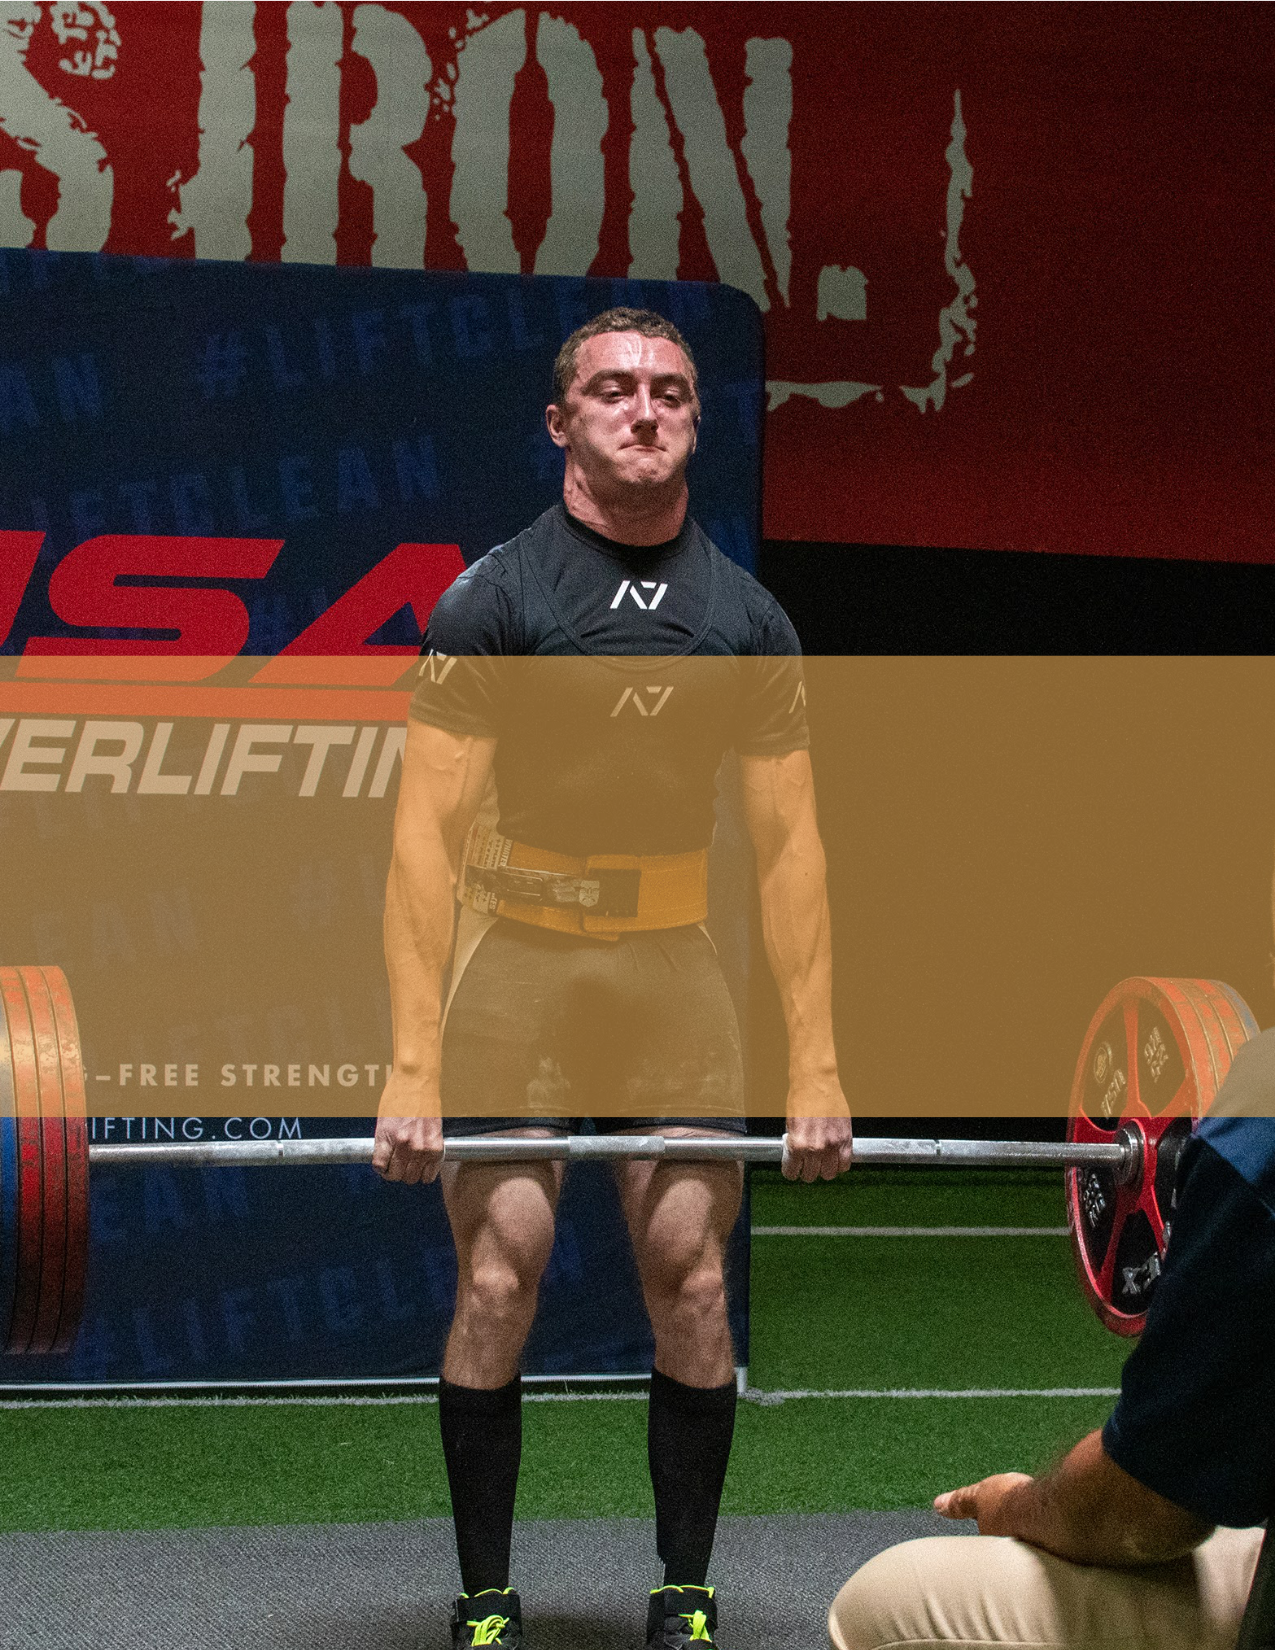
\includegraphics[scale=2.2]{PaperPics/Cover.png}}} % Image background
\centering
\vspace*{8cm}
\par\normalfont\fontsize{35}{35}\sffamily\selectfont
\textbf{Building An Adaptable Training Model}\\
{\LARGE A Mathematical Characterization of a Powerlifting Program}\par % Book title
\vspace*{1cm}
{\Huge Jack Carmichael}\par % Author name
\endgroup

%\AddToShipoutPicture*{\put(0,-60){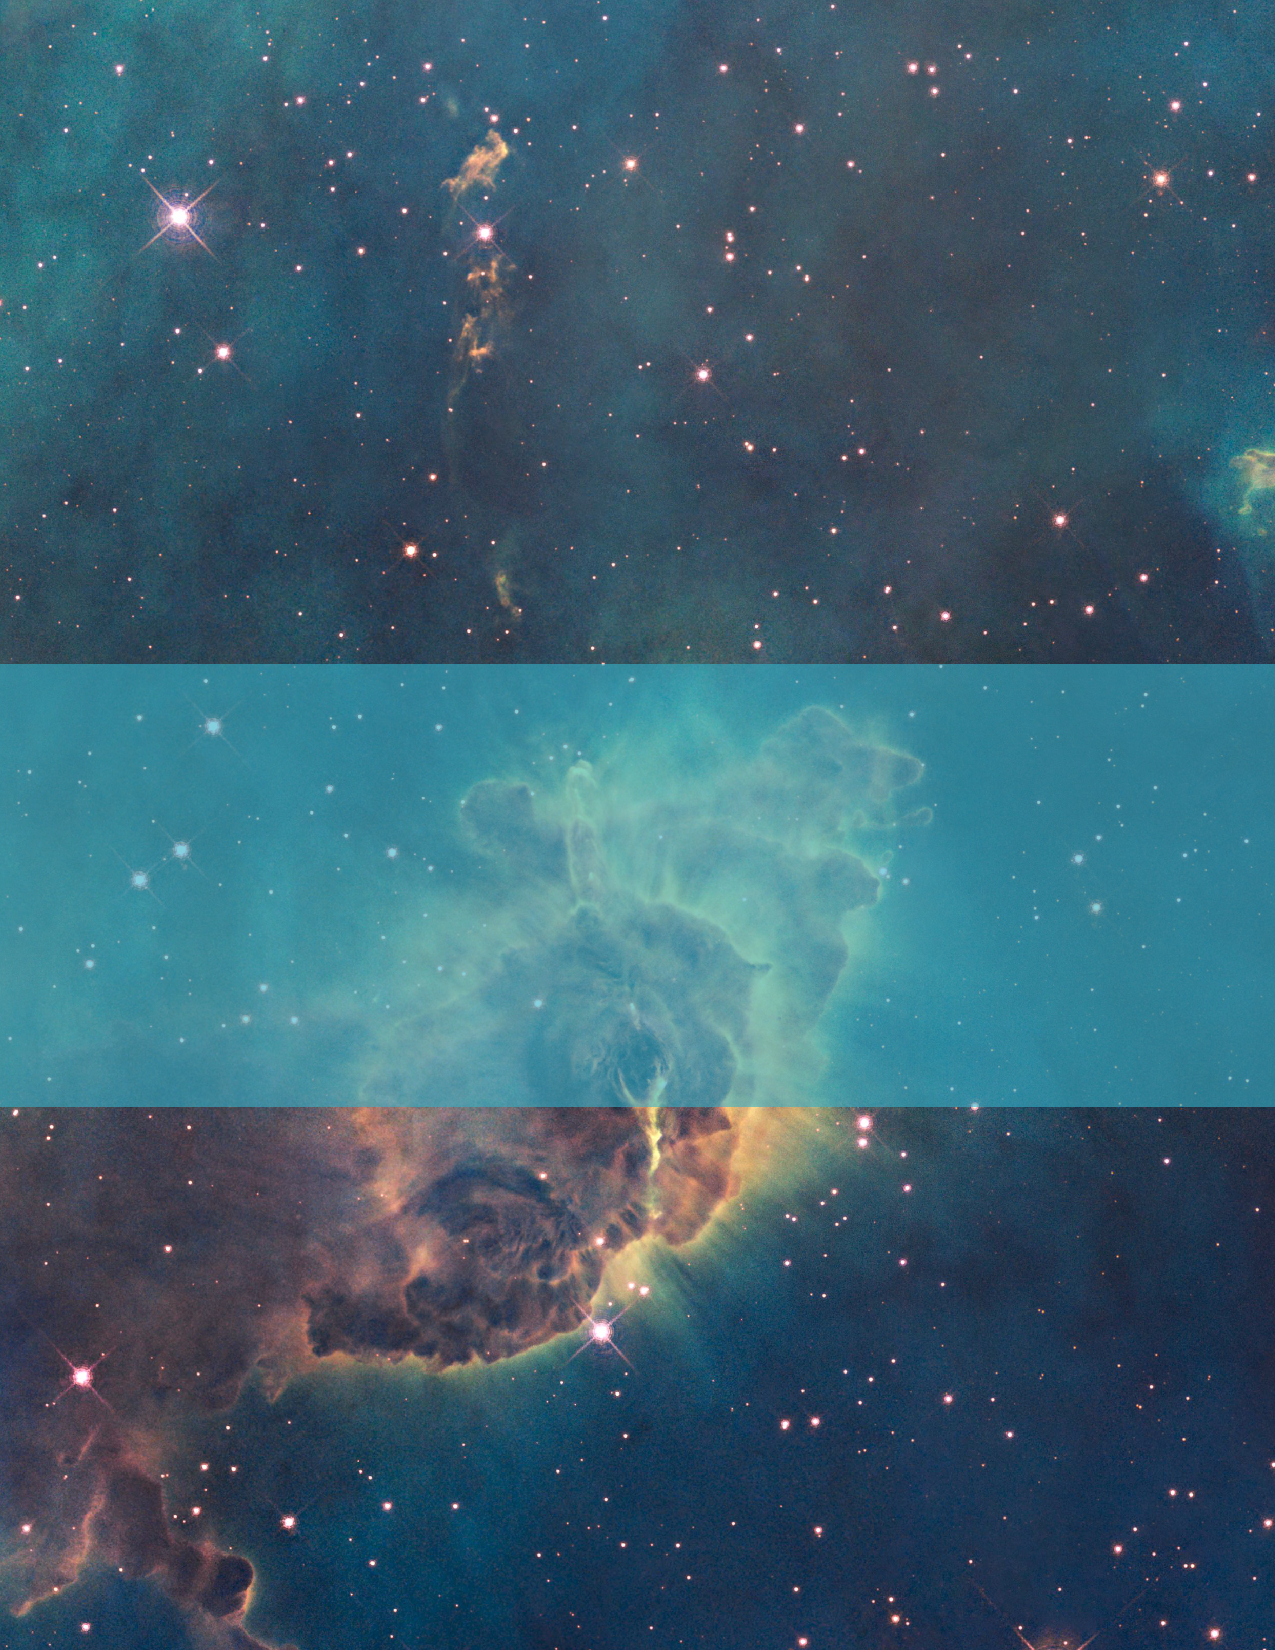
\includegraphics[scale=1.25]{PaperPics/esahubble.png}}} % Image background
% \begingro
% \par
% \normalfont\fontsize{35}{35}\sffamily\selectfont
% \title{\textbf{Building an Adaptable Training Model}\\[1cm]
% Mathematical Characterization of a Powerlifting Program\\[1cm]} 
% \author{Jack Carmichael}
% %\date{\vspace{9cm}\normalsize{\textit{"Besides, it is a disgrace to grow old through sheer carelessness before seeing what manner of man you may become by developing your bodily strength and beauty to their highest limit. But you cannot see that, if you are careless; for it will not come of its own accord."}}\\- Socrates}
% % \date{\vspace{10cm} Colorado School of Mines \\[0.5cm] Mathematics - your class \\[0.5cm] Investigation/IA/EE \\[0.5cm] Word Count: xx}
% \maketitle
%---------------------------------------------------------------------------
\newpage
~\vfill
\thispagestyle{empty}

\vspace*{\fill}
\textit{"Besides, it is a disgrace to grow old through sheer carelessness before seeing what manner of man you may become by developing your bodily strength and beauty to their highest limit. But you cannot see that, if you are careless; for it will not come of its own accord."}\\
\begin{center}
    - Socrates
\end{center}
\vspace*{\fill}
%---------------------------------------------------------------------------
\newpage
\tableofcontents
%---------------------------------------------------------------------------
\newpage
\chapter{Introduction}
\label{sec:Introduction}

Lots of workout programs exist for powerlifters. These tend to be static and do not change in order to adapt to the lifter. Even if a workout program does offer some form of adaptability, it is usually extremely limited.

Yet, not all people respond to training in the same way. For example, some people respond well to high volume and others don't, some people have a lower tolerance to intensity than 'average', and some people cannot perform a certain lift very well due to prior injuries or lack of skill. Even the same lifter does not respond to training the same way across time, requiring continual adjustments to achieve maximum potential. Everybody has optimal constraints that they should strive to work within.

Typically a lifter would hire a coach to manage and adapt there training for them and there current constraints. The goal of this paper is to 'dive into' a coaches mindset and mathematically capture ideas fundamental to the jobs they perform. The hope is that the model outlined in this paper will be sufficient to constitute a training program that a lifter can follow and make progress with.

\section{Outline}

Below is an outline of what each chapter covers.

\begin{enumerate}
    \setcounter{enumi}{1}
    \item \textbf{Data} \\ \textit{The Source of Truth} \\
        This section introduces the data as well as important points inside the data set. While here, units of measurement are discussed to frame future discussions.
    \item \textbf{Potential Surface} \\ \textit{Establishing What's Possible} \\
        This section is where the modeling begins, and defines what is possible for a lifter to complete. While establishing what is possible, it also introduces novel ways to describe what is happening during a workout.
    \item \textbf{Time Frame} \\ \textit{Fine Tuning The Model} \\
        This section is concerned with defining the models state along with how it moves through time to match the changes a lifter is experiencing, allowing the model to adapt to the lifter. While discussing adaptations through time, the models reaction to injuries is also discussed.
\end{enumerate}

\section{Common Terms: Getting on the Same Page}
\label{sec:CommonTermsSection}

Throughout the rest of this paper several terms will be used. Because this paper is going to be read by people outside of the lifting community, some common terminology and concepts will be introduced here. If you are familiar with lifting and the concepts surrounding training, this section can be skipped.

A \textit{workout program} consists of a series of \textit{exercises} to complete on a given day. Exercises vary depending on what a lifter's goals are, amongst other factors. Exercises are composed of \textit{sets}. Sets are composed of \textit{reps}, short for repetitions, making a rep the smallest unit of work in the gym. Given this, an workout program is just a list of exercises to complete over time where each exercise has a specific number of sets and reps to be done at a specific weight. Table \ref{tab:WorkoutProgramExample} exemplifies this.

\begin{table}[h]
    \centering
    \begin{tabular}{c|c|c|c|c|c}
        Date & Exercise & Sets & Reps & Weight & Effort \\
        \hline
        Mon, July 4\textsuperscript{th} & Deadlifts & $6$ & $6$ & $405$ lbs & $8.5$ \\
        Mon, July 4\textsuperscript{th} & Barbell Rows & $5$ & $10$ & $135$ lbs & - \\
        Mon, July 4\textsuperscript{th} & Lat Pulldowns & $5$ & $15$ & $120$ lbs & - \\
        Tue, July 5\textsuperscript{th} & Squat & $3$ & $8$ & $345$ lbs & $9$ \\
        Tue, July 5\textsuperscript{th} & Goblet Squats & $5$ & 15 & $85$ lbs & - \\
        \dots & \dots & \dots & \dots & \dots & \dots \\
    \end{tabular}
    \caption{A table showing how a workout is represented. This data is made up for the purpose of the example.}
    \label{tab:WorkoutProgramExample}
\end{table}

As shown in table \ref{tab:WorkoutProgramExample}, there is one more descriptive element that will give a more complete picture of what is happening across a workout program: \textit{effort}. Every combination of exercises, sets, reps, and weight will be performed at a particular effort. Effort describes how hard a lifter will need to work to complete the prescribed exercise at the given sets, reps, and weight. Effort is generally only used for \textit{compound movements}, or an exercise that requires more than one joint.

Effort will be measured on a scale known as \textit{rate of perceived exertion}, or \textit{RPE}. After every set, a lifter can rate the amount of effort they feel they exerted according to table \ref{tab:RPETable}. The RPE scale is widely used, well researched, and has been proven to be the best method for a lifter to rate the effort required to complete a lift. \cite{RPE_ACCURACY}

\begin{table}[h]
    \centering
    \begin{tabular}{c|l}
        Effort Rating & Description \\
        \hline
        $10$ & All out effort. Could not add weight or reps. \\
        $9.5$ & Could add slightly more weight, could not add reps. \\
        $9$ & Could do one more rep. \\
        $8.5$ & Could definitely do one more rep, possibly two. \\
        $8$ & Could do two more reps. \\
        $7.5 $& Could do two more reps, possibly three. \\
        $7$ & Could do three more reps. \\
        $5-6$ & Could do 4-6 more reps. \\
        $1-4$ & Very light to little effort.
    \end{tabular}
    \caption{A table explaining the relationship between an RPE rating and what the lifter was capable of doing.}
    \label{tab:RPETable}
\end{table}

A workout program is generally categorized into three parts across time: the \textit{macrocycle}, the \textit{mesocycle}, and the \textit{microcycle}. A microcycle has the smallest duration, defining the building blocks that will be repeated to create a training effect, creating the 'rhythm' of the workout program. A microcycle is typically only a week in length. A mesocycle is several microcycles in length. The mesocycle is responsible for changing parameters of the microcycles over time, such as volume and intensity, to create a training effect with respect to a short term goal. The macrocycle defines the duration of the workout program, creating the long term plan that marks milestones and competition dates. The macrocycle is responsible for changing parameters of the mesocycles to create a training effect across the entire rotation and achieve long term goals.

There are three more values that can be calculated from a workout program that combine several elements to describe what is happening at a more abstract level. \textit{Volume} is defined as the product of sets, reps, and weight, shown more formally in equation \ref{eq:BaseVolumeEquation}. Volume represents the total amount of weight lifted, and gives a proxy for the amount of work being done for an exercise.

\begin{equation}
    \label{eq:BaseVolumeEquation}
    v(s,r,w)=srw
\end{equation}

The second value is \textit{intensity}. Intensity is represented as the ratio of the weight lifted to lifters \textit{one rep max}, or \textit{1RM}, for the same exercise. The closer a lifter is to there 1RM on an exercise the greater the intensity of the lift. Equation \ref{eq:BaseIntensityEquation} defines intensity.

\begin{equation}
    \label{eq:BaseIntensityEquation}
    I(w,l_{1RM})=\frac{w}{l_{1RM}}
\end{equation}

With the definition of intensity, equation \ref{eq:BaseVolumeEquation} can be easily be modified to accept intensity values instead of weight.

\begin{equation}
    \label{eq:IntensityBasedVolumeEquation}
    v(s,r,I,l_{1RM})=srIl_{1RM}
\end{equation}

The third value is \textit{frequency}. Frequency is simply how often a lift is performed across a microcycle. Certain exercises respond better to higher frequency than others, and some lifters can tolerate higher frequencies than others.

Another important concept is \textit{fatigue}. As a lifter progresses through a workout program there fatigue will increase. Fatigue is unavoidable, and it must be properly managed. Continually training in a fatigued state will result in far greater chances of sustaining an injury and lackluster progress. \cite{FATIGUE} Fatigue can be managed in many ways such as decreasing intensity, frequency, volume, or taking extra unplanned time off from the gym.

The last concept considered here is the difference between \textit{strength training} and \textit{hypertrophy}. Generally, strength training seeks to maximize a particular set of exercises 1RM's where as hypertrophy seeks to maximize muscle growth. To a certain extent, they go hand in hand, but one can be emphasized over the other. For hypertrophy there are generally fewer sets with more reps and lighter weight. For strength training there are generally more sets with fewer reps and heavier weight. This paper is concerned with powerlifting, which is a strength sport, but hypertrophy can be used as a tool to gain strength so it is important to understand it.
%---------------------------------------------------------------------------

%\chapter{
    Common Terms
    \\
    \large{Getting on the Same Page}
}
\label{sec:CommonTermsSection}

Throughout the rest of this paper several terms will be used. Because this paper is going to be read by people outside of the lifting community, some common terminology and concepts will be introduced here. If you are familiar with lifting and the concepts surrounding training, this section can be skipped.

A \textit{workout program} consists of a series of \textit{exercises} to complete on a given day. Exercises vary depending on what a lifter's goals are, amongst other factors. Exercises are composed of \textit{sets}. Sets are composed of \textit{reps}, short for repetitions, making a rep the smallest unit of work in the gym. Given this, an workout program is just a list of exercises to complete over time where each exercise has a specific number of sets and reps to be done at a specific weight. Table \ref{tab:WorkoutProgramExample} exemplifies this.

\begin{table}[h]
    \centering
    \begin{tabular}{c|c|c|c|c|c}
        Date & Exercise & Sets & Reps & Weight & Effort \\
        \hline
        Mon, July 4\textsuperscript{th} & Deadlifts & $6$ & $6$ & $405$ lbs & $8.5$ \\
        Mon, July 4\textsuperscript{th} & Barbell Rows & $5$ & $10$ & $135$ lbs & - \\
        Mon, July 4\textsuperscript{th} & Lat Pulldowns & $5$ & $15$ & $120$ lbs & - \\
        Tue, July 5\textsuperscript{th} & Squat & $3$ & $8$ & $345$ lbs & $9$ \\
        Tue, July 5\textsuperscript{th} & Goblet Squats & $5$ & 15 & $85$ lbs & - \\
        \dots & \dots & \dots & \dots & \dots & \dots \\
    \end{tabular}
    \caption{A table showing how a workout is represented. This data is made up for the purpose of the example.}
    \label{tab:WorkoutProgramExample}
\end{table}

As shown in table \ref{tab:WorkoutProgramExample}, there is one more descriptive element that will give a more complete picture of what is happening across a workout program: \textit{effort}. Every combination of exercises, sets, reps, and weight will be performed at a particular effort. Effort describes how hard a lifter will need to work to complete the prescribed exercise at the given sets, reps, and weight. Effort is generally only used for \textit{compound movements}, or an exercise that requires more than one joint.

Effort will be measured on a scale known as \textit{rate of perceived exertion}, or \textit{RPE}. After every set, a lifter can rate the amount of effort they feel they exerted according to table \ref{tab:RPETable}. The RPE scale is widely used, well researched, and has been proven to be the best method for a lifter to rate the effort required to complete a lift. \cite{RPE_ACCURACY}

\begin{table}[h]
    \centering
    \begin{tabular}{c|l}
        Effort Rating & Description \\
        \hline
        $10$ & All out effort. Could not add weight or reps. \\
        $9.5$ & Could add slightly more weight, could not add reps. \\
        $9$ & Could do one more rep. \\
        $8.5$ & Could definitely do one more rep, possibly two. \\
        $8$ & Could do two more reps. \\
        $7.5 $& Could do two more reps, possibly three. \\
        $7$ & Could do three more reps. \\
        $5-6$ & Could do 4-6 more reps. \\
        $1-4$ & Very light to little effort.
    \end{tabular}
    \caption{A table explaining the relationship between an RPE rating and what the lifter was capable of doing.}
    \label{tab:RPETable}
\end{table}

A workout program is generally categorized into three parts across time: the \textit{macrocycle}, the \textit{mesocycle}, and the \textit{microcycle}. A microcycle has the smallest duration, defining the building blocks that will be repeated to create a training effect, creating the 'rhythm' of the workout program. A microcycle is typically only a week in length. A mesocycle is several microcycles in length. The mesocycle is responsible for changing parameters of the microcycles over time, such as volume and intensity, to create a training effect with respect to a short term goal. The macrocycle defines the duration of the workout program, creating the long term plan that marks milestones and competition dates. The macrocycle is responsible for changing parameters of the mesocycles to create a training effect across the entire rotation and achieve long term goals.

There are three more values that can be calculated from a workout program that combine several elements to describe what is happening at a more abstract level. \textit{Volume} is defined as the product of sets, reps, and weight, shown more formally in equation \ref{eq:BaseVolumeEquation}. Volume represents the total amount of weight lifted, and gives a proxy for the amount of work being done for an exercise.

\begin{equation}
    \label{eq:BaseVolumeEquation}
    v(s,r,w)=srw
\end{equation}

The second value is \textit{intensity}. Intensity is represented as the ratio of the weight lifted to lifters \textit{one rep max}, or \textit{1RM}, for the same exercise. The closer a lifter is to there 1RM on an exercise the greater the intensity of the lift. Equation \ref{eq:BaseIntensityEquation} defines intensity.

\begin{equation}
    \label{eq:BaseIntensityEquation}
    I(w,l_{1RM})=\frac{w}{l_{1RM}}
\end{equation}

With the definition of intensity, equation \ref{eq:BaseVolumeEquation} can be easily be modified to accept intensity values instead of weight.

\begin{equation}
    \label{eq:IntensityBasedVolumeEquation}
    v(s,r,I,l_{1RM})=srIl_{1RM}
\end{equation}

The third value is \textit{frequency}. Frequency is simply how often a lift is performed across a microcycle. Certain exercises respond better to higher frequency than others, and some lifters can tolerate higher frequencies than others.

Another important concept is \textit{fatigue}. As a lifter progresses through a workout program there fatigue will increase. Fatigue is unavoidable, and it must be properly managed. Continually training in a fatigued state will result in far greater chances of sustaining an injury and lackluster progress. \cite{FATIGUE} Fatigue can be managed in many ways such as decreasing intensity, frequency, volume, or taking extra unplanned time off from the gym.

The last concept considered here is the difference between \textit{strength training} and \textit{hypertrophy}. Generally, strength training seeks to maximize a particular set of exercises 1RM's where as hypertrophy seeks to maximize muscle growth. To a certain extent, they go hand in hand, but one can be emphasized over the other. For hypertrophy there are generally fewer sets with more reps and lighter weight. For strength training there are generally more sets with fewer reps and heavier weight. This paper is concerned with powerlifting, which is a strength sport, but hypertrophy can be used as a tool to gain strength so it is important to understand it.
\chapter{
    Data
    \\
    \large{The Source of Truth}
}
\label{sec:DataSection}

The data associated with this paper is present in the projects associated GitHub repository, available at the following url:  \url{github.com/carmichaeljr/powerlifting-engine}.
The data represents almost two years worth of training data, all collected from a single lifter. There are over 900 data points in this data set varying across many different exercises. Before recording any data, the lifter was asked to list there 1RM's for several lifts. These were recorded as having been performed on macrocycle 1 and having RPE 10.

The data recorded consists of a list of exercises performed at the gym, with the lifter recording the following data for each exercise:

\begin{itemize}
    \item What exercise was performed
    \item The weight the exercise was performed at
    \item The number of sets that were performed
    \item The number of reps that were performed
    \item The date the exercise was performed on
    \item The RPE the exercise required
\end{itemize}

In addition to the data listed above, the lifter also recorded the starting and ending dates of each macrocycle. From the data the lifter recorded, the following additional data points were calculated. These data points were calculated for the lifter in order to avoid any errors from manual entry.

\begin{itemize}
    \item The volume for each exercise was obtained by multiplying the sets, reps, and weight. This comes directly from equation \ref{eq:BaseVolumeEquation}.
    \item The intensity for each exercise was calculated in relation to the best lift of the same exercise in the previous macrocycles. This comes directly from equation \ref{eq:BaseIntensityEquation}.
    \item Each lift was given a macrocycle ID according to the date the exercise was performed.
\end{itemize}

During the time period the lifter was recording data, there were several notable occurrences:

\begin{enumerate}
    \item Near 3/2/2022 the lifter sustained an injury to there lower back, specifically there sacroiliac joint, or SI joint. This injury was a result of rounding of the lumbar spine while attempting a maximal effort deadlift, and required chiropractic care coupled with 2 weeks off of training. The failed lift was not recorded.
    
    \item On 5/5/2022 the lifter participated in a deadlift only competition. The 5 week prep leading up to that competition was very successful, and resulted in the lifter getting a 20 lb PR on the deadlift.
    
    \item On 7/24/2022 the lifter participated in a full meet. The prep leading up to that competition was very consistent, and resulted in the lifters best performance on the platform to date.
    
    \item On 10/5/2022 the lifter tore there hamstring squatting. The diagnosis was a grade 1-2 muscle belly tear, and the lifter went to three physical therapy (PT) sessions before feeling comfortable to adjust training on there own.
\end{enumerate}

\section{Units of Measurement}
\label{sec:UnitsOfMeasurement}

Before starting, it is worth mentioning how elements in the data set were measured as it will set the stage for future discussion.

Weight, and hence intensity, are obvious. Recording the weight lifted and the fraction that weight is of the lifters 1RM is all that's required. This defines weight as $w> 0$ and intensity as $I>0$. Weight is not allowed to equal $0$ because that would imply there is no resistance and hence no training stimulus, making the exercise useless. \footnote{Sometimes people classify body weight exercises as having $0$ weight, despite still having to lift some fraction of there own body weight. This is mainly done because it can be difficult to measure the exact proportion of there body weight they are actually lifting.} Intensity is not capped at $1$ because lifting a weight greater than the lifters previous 1RM is the ultimate goal of a powerlifting program.

Reps are just positive integer values greater than or equal to $1$, or $r\in \{ \mathbb{R}\ge 1 \}$. As mentioned in section \ref{sec:CommonTermsSection}, effort will follow the RPE scale, defining effort as $E\in \{0,0.5,1,...,10\}$.

Time will be recorded as a date, which means it will have units of days. Dates by themselves cannot be mathematically used. To work around this, the past will be positive values representing the number of days since the exercise was performed. This will make $0$ represent the current day. Given this, time will be in the domain of positive integer values, or $t\in \{ \mathbb{R}\ge 0 \}$.

Following the traditional definition, frequency will be calculated across days, meaning separate sets of the same exercise on the same day will not count toward an increased frequency. Separate sets of the same exercise on different days will increase the frequency of the exercise. Naturally, frequency is limited to positive integer values, or $f\in \{ \mathbb{R}\ge 0 \}$.

Sets appear to be in the same domain as reps, but a specific case leads to a different representation. Lets say a lifter is prescribed to squat for $5$ sets of $3$ with the same weight across all $5$ sets. The exact weight is not relevant to the example. Then lets say the lifter completed all $3$ reps on the first $4$ sets, but only managed to complete $2$ reps on the last set. One way to record this is shown in table \ref{tab:FailedSetExampleIncorrectData}.

\begin{table}[h]
    \centering
    \begin{tabular}{c|c|c|c}
        Exercise & Sets & Reps & \dots \\
        \hline
        Squat & $4$ & $3$ & \dots \\
        Squat & $1$ & $2$ & \dots \\ 
    \end{tabular}
    \caption{A table illustrating the incorrect way to record failed reps across sets.}
    \label{tab:FailedSetExampleIncorrectData}
\end{table}

Recording the missed rep this way will lead to problems later when attempting to fit a surface to the data, as a single data point will have turned into two correlated data points. \footnote{Linear regression assumes that the data points are independent from each other.} Put another way, the same exercise now has two data points. To remedy this, fractional sets will be used, making sets in the domain of positive numbers greater than or equal to $1$, or $s\ge 1$. The reason sets cannot be less than $1$ is because any fractional sets less than one can simply be represented as a single set of less reps. Table \ref{tab:FailedSetExampleCorrectData} shows the adjusted way to record failed reps.

\begin{table}[h]
    \centering
    \begin{tabular}{c|c|c|c}
        Exercise & Sets & Reps & \dots \\
        \hline
        Squat & $4\frac{2}{3}$ & 3 & \dots \\
    \end{tabular}
    \caption{A table illustrating the correct way to record failed reps across sets.}
    \label{tab:FailedSetExampleCorrectData}
\end{table}

Note that volume, as shown below, is not changed by making sets fractional. Intensity is not changed in virtue of the weight not changing and frequency is also not changed due to the sets all being performed on the same day.

\begin{equation*}
    \begin{split}
        v_1=&v(4,3,w)+v(1,2,w)=14w \\
        v_2=&v\left(4\frac{2}{3},3,w\right)=14w \\
    \end{split}
\end{equation*}
\chapter{
    Potential Surface
    \\
    \large{Establishing What's Possible}
}
\label{sec:PotentialSurface}

As stated in the introduction, every person responds to lifting differently. This section is concerned with finding and establishing the limits of a given lifter within the context of a single exercise.

There are many limiting factors that need to be considered. How many reps can be done per set? How many sets can be done per exercise? What weight can the user lift given a particular amount of sets and reps? How much effort should the lifter exert to perform those sets and reps at the given weight? The answers to these questions form the thought process for the rest of the section.

When performing a single exercise, there are generally six things that dictate what is done:
\begin{enumerate}
    \item What exercise is being performed
    \item The number of sets being performed for a particular exercise
    \item The number of reps being performed for each set
    \item The weight each rep should be performed at
    \item The amount of effort expected to be exerted on each set
    \item The lifters current abilities
\end{enumerate}

The exercise being performed is largely dependent on what goals the lifter is pursuing as well as what weaknesses the lifter has. Due to the complexity of exercise selection as well as it's independence from the last five items on the list, it is explored in greater detail in a separate section. The last five items on that list have a large amount of dependence upon each other, and the relationship among them will be established in this section.

\section{Intuitive Relationships Between Variables}
\label{sec:PotentialSurfaceIntuitiveRelationshipsBetweenVariables}

A lifter has a \textit{volume tolerance}, which represents a lifters work capacity. Given a certain volume tolerance, the only five variables that can change are weight, intensity, effort, sets, and reps. This is obvious from equations \ref{eq:BaseVolumeEquation} and \ref{eq:IntensityBasedVolumeEquation}.

Weight and intensity are synonymous through the lens of volume, as the total amount of weight lifted is calculated regardless of the differing parameters. It should be clear from equations \ref{eq:BaseVolumeEquation} and \ref{eq:IntensityBasedVolumeEquation} that volume will increase with increased weight and intensity. Mathematically, this makes sense, but the limits of the human body need to be considered. As intensity approaches $100\%$ more effort is required to maintain the same amount of volume. Because effort is limited, volume will necessarily decrease at higher weights, to a point where it reverses the increase in volume from the increase in weight. An example may make this clearer. At $100\%$ intensity a lifter can realistically expect to obtain a volume equal to there 1RM, shown in equation \ref{eq:VolumeWithDiffereingIntensities1}. At $50\%$ intensity, all it takes is two reps to match the volume performed at $100\%$ intensity, which is shown in equation \ref{eq:VolumeWithDiffereingIntensities2}. At $50\%$ intensity, far more than one set of two reps can be performed, making it easy to surpass the volume done at $100\%$ intensity. The data in appendix \ref{sec:AppendixA} has many examples of this.

\begin{subequations}
    \begin{align}
        \label{eq:VolumeWithDiffereingIntensities1}
        v_{I=1}=&v(1,1,l_{1RM})=l_{1RM} \\
        \label{eq:VolumeWithDiffereingIntensities2}
        v_{I=0.5}=&v(1,2,0.5l_{1RM})=l_{1RM}
    \end{align}
\end{subequations}

It should be clear that volume will increase with weight until a peak is reached and from there will start to decrease because of limited effort at higher intensities. Where volume peaks exactly will need to be found from the data. Figure \ref{fig:IntensityVsVolumeGraph} is a graph comparing intensity and volume that clearly displays the intuitive behaviors discussed above.

\begin{figure}
    \centering
    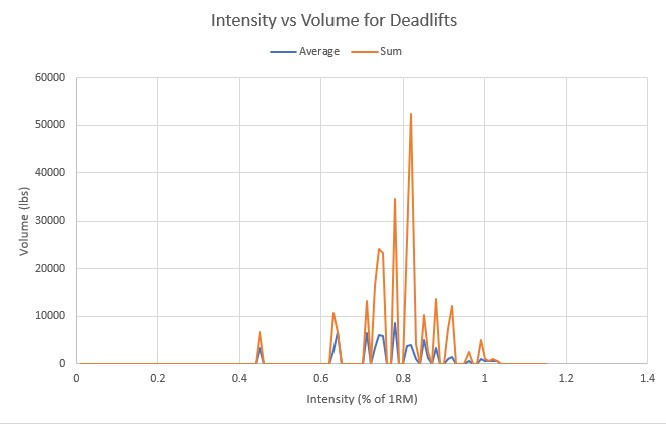
\includegraphics[scale=1.6]{graphs/IntensityVsVolumeGraph.jpg}
    \caption{A graph comparing intensity and volume. Note how there is a clear peak in volume near $80\%$.}
    \label{fig:IntensityVsVolumeGraph}
\end{figure}

With volume diminishing due to limited effort at higher intensities, the next question is what happens when effort increases or decreases across all intensities. As effort increases, more sets will be able to be completed, more reps will be able to be completed in each set, or more weight will be able to be lifted. If the increase in effort is large enough, some combination of sets, reps, and weight could all increase. The opposite is true if effort decreases. Again, from equations \ref{eq:BaseVolumeEquation} and \ref{eq:IntensityBasedVolumeEquation} it should be clear that sets and reps are directly proportional to volume, implying an increase in either one will increase volume. Putting all of this together, as effort increases volume will increase and as effort decreases volume will decrease.

\begin{figure}
    \centering
    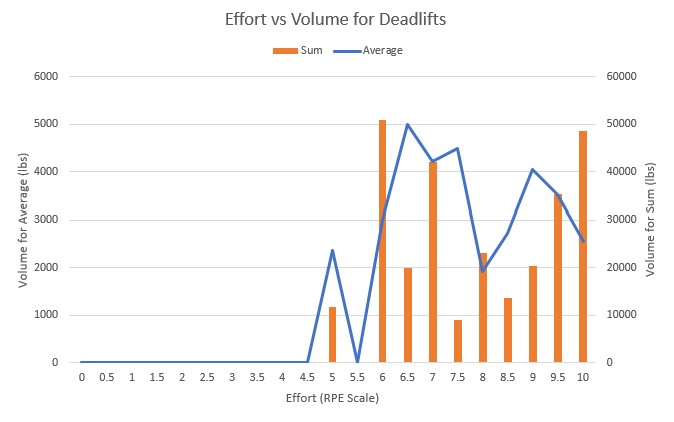
\includegraphics[scale=1.6]{graphs/EffortVsVolumeGraph.jpg}
    \caption{A graph comparing effort and volume. Note how volume tends to increase with higher effort values. The drop in volume at $E>7$ is likely from greater efforts generally having greater intensity, as shown in figure \ref{fig:EffortVsIntensity}.}
    \label{fig:EffortVsVolumeGraph}
\end{figure}
\begin{figure}
    \centering
    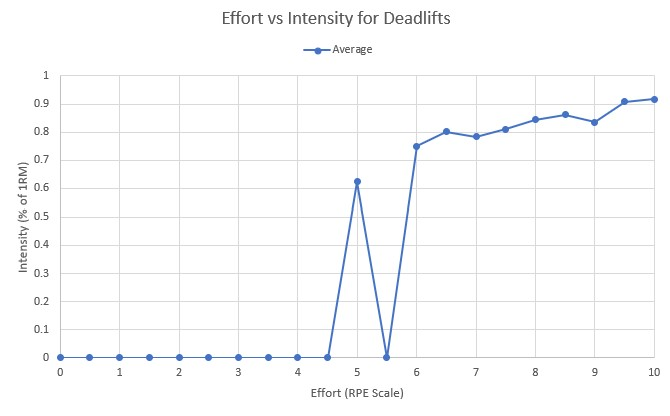
\includegraphics[scale=1.6]{graphs/EffortVsIntensityGraph.jpg}
    \caption{A graph comparing effort and average intensity. Note how the average intensity tends to increase with higher effort values. This is the result of a powerlifters goal being to maximize a 1RM. There are no data points in the range $0\le E\le 4.5$, making the average $0$.}
    \label{fig:EffortVsIntensity}
\end{figure}

In figure \ref{fig:EffortVsVolumeGraph} volume does seem to increase with effort, but after about $E=7$ it appears to decrease. This is a result of effort and intensity being correlated, which is shown in figure \ref{fig:EffortVsIntensity}. Effort and intensity being correlated is an artifact of the data being collected by a powerlifter, where the goal is to maximize the 1RM for a particular lift. As effort increases, a powerlifter will seek to maximize weight over volume. Combining the goal to maximize weight, and volume at higher intensities being necessarily limited by effort, the drop in volume after $E=7$ shown in figure \ref{fig:EffortVsVolumeGraph} is fully explained. Given a sport that is more concerned with rep maxes, such as crossfit, the effort vs intensity graph would level out because lower intensities would be pushed for as many reps as possible, creating a maximal effort set with a lower intensity. This would remove the drop in volume shown in the effort vs volume graph because higher effort sets would be performed with lower intensities that would allow the volume to continue to increase. This is also a perfect example to demonstrate how effort and intensity are two different concepts.

At this point, it may be tempting to conclude that volume should be constant given a particular weight and effort. This conclusion can be reached by looking at equations \ref{eq:BaseVolumeEquation} and \ref{eq:IntensityBasedVolumeEquation}, where once the weight and effort are known sets and reps would just vary inversely to ensure volume remains constant. Again, while mathematically true, the limits of the human body need to be considered. Evidence that the relationship between sets and reps is not inverse is shown in figure \ref{fig:SetsVsReps}, where a drop in reps from the expected inverse pattern is seen for $s<3$. This can be attributed to a lack of \textit{endurance}, where sets with a greater number of reps  require more endurance than sets with less reps. Powerlifters are eternally known for having no endurance, so it should come as no surprise that they will favor more sets over reps. This favoritism between sets and reps will of course mean volume is no longer constant given a particular weight and effort, and as such will be known as the \textit{volume skew}.

\begin{figure}[h]
    \centering
    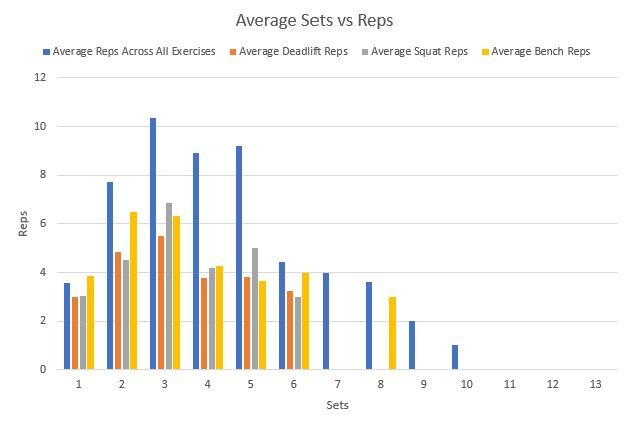
\includegraphics[scale=1.6]{graphs/SetsVsRepsGraph.jpg}
    \caption{A graph comparing average reps and sets. Note how the relationship is not perfectly inverse. In this case, the lifter has a volume skew towards sets, where more sets are favored (the long tail to the right), over reps (which would require a shorter tail and greater peak).}
    \label{fig:SetsVsReps}
\end{figure}

By this point it should be obvious the crux of the problem in question will require finding a lifters volume tolerance across weight and effort, as well as the lifters volume skew between sets and reps.

\section{Linear Regression and Time Series Problems}
\label{sec:PotentialSurfaceLinearRegressionAndTimeSeriesProblems}

With the goal to find a surface of best fit using the data set and linear regression, the limits of linear regression need to be considered. Looking at the data set, it should be clear that it is a time series: the data points are collected over time, and data points nearer in time have greater importance than data points farther away in time. Linear regression assumes that all the data points are uncorrelated, which was just proved to not be true. To reconcile the differences between working with linear regression and a time series data set, two things can be done.

The first step that can be taken is to limit the time frame that linear regression is run over. Sets, reps, volume, and the volume skew can all vary through time, but not necessarily in direct relation to time. As an example of this, consider seasonal training, which some powerlifters choose to employ. In the off season intensities will drop, volume will increase, and the emphasis on training may shift to hypertrophy over strength. In the on season intensities will increase, volume will necessarily decrease, and the emphasis on training will shift to strength over hypertrophy. This will result in shifts in the number of sets and reps being done over time. To capture these changes over time, the data points used will be limited to a specific time frame creating a form of a moving average as a lifter continues to train. Equation \ref{eq:TimeFrame} will be used to determine if a data point should be used while performing linear regression. The exact length of the time frame, $t_f$, will be discussed in section \ref{sec:TimeFrame}. Throughout the rest of this paper, equation \ref{eq:TimeFrame} will be written short hand as $t_i\in \{ T \}$.

\begin{equation}
    \label{eq:TimeFrame}
    \begin{split}
        %t_t\le t_i\le t_t+t_f
        t_i & \in\{ t_t, t_t+1,\dots,t_t+t_f \} \\
        \equiv t_i & \in \{ T \}
    \end{split}
\end{equation}
\centerline{where}
\begin{equation*}
    \begin{split}
        t_i &\equiv \text{The time component of an arbitrary data point }i \\
        t_t &\equiv \text{An arbitrary target time} \\
        t_f &\equiv \text{The time frame linear regression will be run over} \\
        T & \equiv \text{A shorthand notation representing the set of all allowed times}
    \end{split}
\end{equation*}

The second step that can be taken is to remove weights correlation with time. Weight correlating with time makes intuitive sense, as the goal of a powerlifter is to continually increase weight over time. As an example, say a lifter starts out with a 1RM of $300$ lbs on squat, but through training is able to increase that weight over time to $800$ lbs. It should be obvious from the example that weight has a positive correlation with time. To fix this, weight will be replaced by intensity. This will remove the correlation with time because intensity is calculated using an exercises 1RM, which itself changes with time, canceling out any effects from an increase in weight as time increases. Going back to the previous example, despite weight increasing over time, intensity would generally be limited to the range $0\le I\le 1$, because the lifter would set new 1RM's over time thereby forcing the intensities to be generally less than $1$.

By replacing weight with intensity, having an accurate tracking of a lifters 1RM over time becomes an important dependence for the model. For a powerlifter, this is generally not a problem as a lifts 1RM is usually tested once a mesocycle. Problems arise however when things like injuries, or other unplanned problems occur. During these situations a lifters 1RM is not known and can change rapidly or extremely slowly over time. A solution to problems like this will be explored in section \ref{sec:TimeFrameDynamicTimeFrameAnalysis} and \ref{sec:TimeFrameInjuriesAndChanges}.

\section{Defining the Relationships}
\label{sec:PotentialSurfaceDefiningTheRelationships}

To find a surface and run linear regression, the following subset of the data set is need.

\begin{equation}
    \label{eq:UserDataSet}
    \begin{split}
        \{(s,r,I,E)_i\}_{i=0}^n & \text{  where}\\
        \begin{split}
            s&\equiv \text{Sets} \\
            r&\equiv \text{Reps} \\
            I&\equiv \text{Intensity} \\
            E&\equiv \text{Effort} \\
        \end{split}
    \end{split}
\end{equation}

The inverse relationship between sets and reps mentioned in section \ref{sec:PotentialSurfaceIntuitiveRelationshipsBetweenVariables} leads to an initial representation of $sr=I$. This cannot be used however because of the asymptotic behavior of the equation at $x=0$ and $y=0$. It is not physically possible for a lifter to continually do infinitely more reps with infinitely less sets, or visa versa. This equation is also to rigid to account for any volume skew. The equation $s^2+r^2=I$ avoids asymptotic behavior and also allows for volume to be skewed, but can lead to a large peak in volume that cannot be controlled without reducing volume across the board. \footnote{This is the classical optimization problem presented in algebra classes, where the optimization equation is a parabola. In this case, the parabolic nature of the optimization equation, which represents some quasi-measure of volume, has to much 'volume' as the peak of the parabola is approached. A more level 'volume' equation is desired.} To avoid both problems, a combination of the equations will be used, which is shown below.

%The inverse relationship between sets and reps is mostly preserved, but the asymptotic behavior is also avoided.\footnote{The terms of the inverse relationship are both squared to make solving for $s$ and $r$ easier, which is something that will need to be done later.}

\begin{equation*}
    a(s-1)^2(r-1)^2+b(s-1)^2+c(r-1)^2=1-I
\end{equation*}

The above equation is negated so volume increases as intensity decreases and centered at $(s=1,r=1,I=1)$ to represent the users current 1RM. The constants $a$, $b$, and $c$ are left to be found by fitting the surface to the lifters data.

Effort also needs to be considered. The above equation could just be limited to fit a certain effort, or range of efforts, generating a set of equations, one for each effort or effort range. This sounds good initially, but the sparseness of the data set makes this approach prone to error. A given exercise may only be performed once per week, which gives very little data to work with in a four dimensional problem. Assuming perfect consistency, only 52 data points would be generated over a year. It is clear that every data point needs to be used if possible. Instead of only fitting the surface to data points that have a certain effort, the surface will be fit to all data points with an error proportional to the effort. Another constant, $d$, will be added so that the surface peaks at a weight that is appropriate for the target effort.

\begin{equation}
    \label{eq:PotentialSurfaceEquation}
    a(s-1)^2(r-1)^2+b(s-1)^2+c(r-1)^2+\epsilon E=d-I
\end{equation}
\centerline{where}
\begin{equation*}
    \begin{split}
        E & \in \{ 0,0.5,1,1.5,...,10 \} \\
        a,b,c,d & \ge 0 \\
    \end{split}
\end{equation*}

Equation \ref{eq:PotentialSurfaceEquation} is the final equation that fully realises all of the intuitive relationships discussed in section \ref{sec:PotentialSurfaceIntuitiveRelationshipsBetweenVariables}. This claim will be validated in sections \ref{sec:PotentialSurfaceVolumePeak} and \ref{sec:PotentialSurfaceVolumeIncreasesWithEffort}. Constraints have also been added to the constants in equation \ref{eq:PotentialSurfaceEquation} to limit the behavior of the model to what is sensible for the problem at hand. Keeping in mind the limitations discussed in section \ref{sec:PotentialSurfaceLinearRegressionAndTimeSeriesProblems}, linear regression can now be used to fit the surface to a lifters data, fully defining what that lifter is capable of doing.

The error equation is shown below.

\begin{equation*}
    E_{rr}=\sum_{
            \substack{i=0\\ t_i\in \{ T \}}
        }^n \left(
        I_i
        -d
        +a(s_i-1)^2(r_i-1)^2
        +b(s_i-1)^2
        +c(r_i-1)^2
        +\epsilon E
    \right)^2
\end{equation*}

The partial derivatives of each unknown constant are found, setting each equal to zero to minimize the error.

\begin{equation*}
    \begin{split}
        \frac{\partial E_{rr}}{\partial d}=
        \frac{\partial}{\partial d}\sum_{
                \substack{i=0\\ t_i\in \{ T \}}
            }^n \left(
            I_i
            -d
            +a(s_i-1)^2(r_i-1)^2
            +b(s_i-1)^2
            +c(r_i-1)^2
            +\epsilon E_i
        \right)^2&=0\\
        -2\sum_{
                \substack{i=0\\ t_i\in \{ T \}}
            }^n \left(
            I_i
            -d
            +a(s_i-1)^2(r_i-1)^2
            +b(s_i-1)^2
            +c(r_i-1)^2
            +\epsilon E_i
        \right)&=0\\
        d \sum_{\substack{i=0\\ t_i\in \{ T \}}}^n 1 
        -a \sum_{\substack{i=0\\ t_i\in \{ T \}}}^n (s_i-1)^2(r_i-1)^2
        -b \sum_{\substack{i=0\\ t_i\in \{ T \}}}^n (s_i-1)^2
        -c \sum_{\substack{i=0\\ t_i\in \{ T \}}}^n (r_i-1)^2
        -\epsilon \sum_{\substack{i=0\\ t_i\in \{ T \}}} E_i
        &=
        \sum_{\substack{i=0\\ t_i\in \{ T \}}}^n I_i\\
    \end{split}
\end{equation*}

After a similar process is carried out for each unknown constant, equation \ref{eq:LinearRegMatrixEquation} can be used, and the unknown constants can be solved for.

\begin{equation}
    \label{eq:LinearRegMatrixEquation}
    \left[
    \begin{matrix}
        \sum_{i=0}^n 1 &
        \dots &
        -\sum_{\substack{i=0\\ t_i\in \{ T \}}}^n E_i \\

        \sum_{\substack{i=0\\ t_i\in \{ T \}}}^n (s_i-1)^2(r_i-1)^2 &
        \dots &
        -\sum_{\substack{i=0\\ t_i\in \{ T \}}}^n E_i (s_i-1)^2(r_i-1)^2\\

        \vdots &
        \ddots &
        \vdots \\
        
        \sum_{\substack{i=0\\ t_i\in \{ T \}}}^n E_i &
        \dots &
        -\sum_{\substack{i=0\\ t_i\in \{ T \}}}^n E_i^2
    \end{matrix}
    \right]
    \left[
    \begin{matrix}
        d \\ a \\ \vdots \\ \epsilon
    \end{matrix}
    \right]=\left[
    \begin{matrix}
        \sum_{\substack{i=0\\ t_i\in \{ T \}}}^n I_i \\
        \sum_{\substack{i=0\\ t_i\in \{ T \}}}^n I_i(s_i-1)^2(r_i-1)^2 \\
        \vdots \\
        \sum_{\substack{i=0\\ t_i\in \{ T \}}}^n I_i E_i
    \end{matrix}
    \right]
\end{equation}

With equations \ref{eq:PotentialSurfaceEquation} and \ref{eq:LinearRegMatrixEquation} as well as the data set defined in equation \ref{eq:UserDataSet}, the surface that establishes what is possible for a lifter is fully defined. This surface will be called the \textit{potential surface}, and it is important to conceptualize that every combination of sets, reps, weight, and effort defined by this surface is theoretically possible for a lifter to complete. This is the base future sections of this paper will build off of.

After fitting the surface to the data shown in appendix \ref{sec:AppendixA} and discussed in section \ref{sec:DataSection}, graphs similar to the ones shown in table \ref{tab:DeadliftPotentialSurfaceAcrossEffort} were created. A full set of potential surface graphs for squat, bench, and deadlift across effort levels $5-10$ are available in appendix \ref{sec:AppendixB}. It is important the relationships discussed in section \ref{sec:PotentialSurfaceIntuitiveRelationshipsBetweenVariables} are present in these graphs, which will be the topic for sections \ref{sec:PotentialSurfaceVolumePeak}-\ref{sec:PotentialSurfaceUnboundedVolume}.

\begin{table}[]
    \centering
    \begin{tabular}{c|c}
        RPE & Potential Surface Graph \\
        \hline \\
        
        5 &
        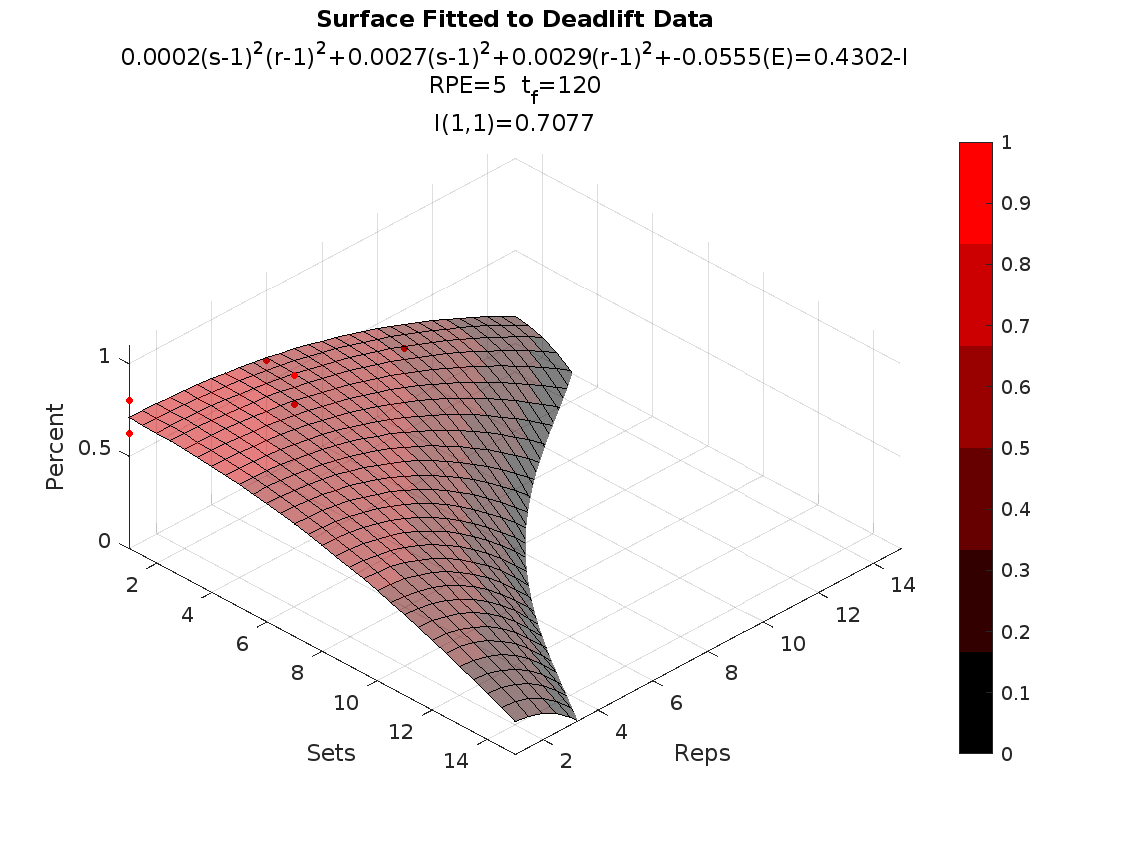
\includegraphics[width=139mm]{DeadliftSurface/5.png} \\
        10 &
        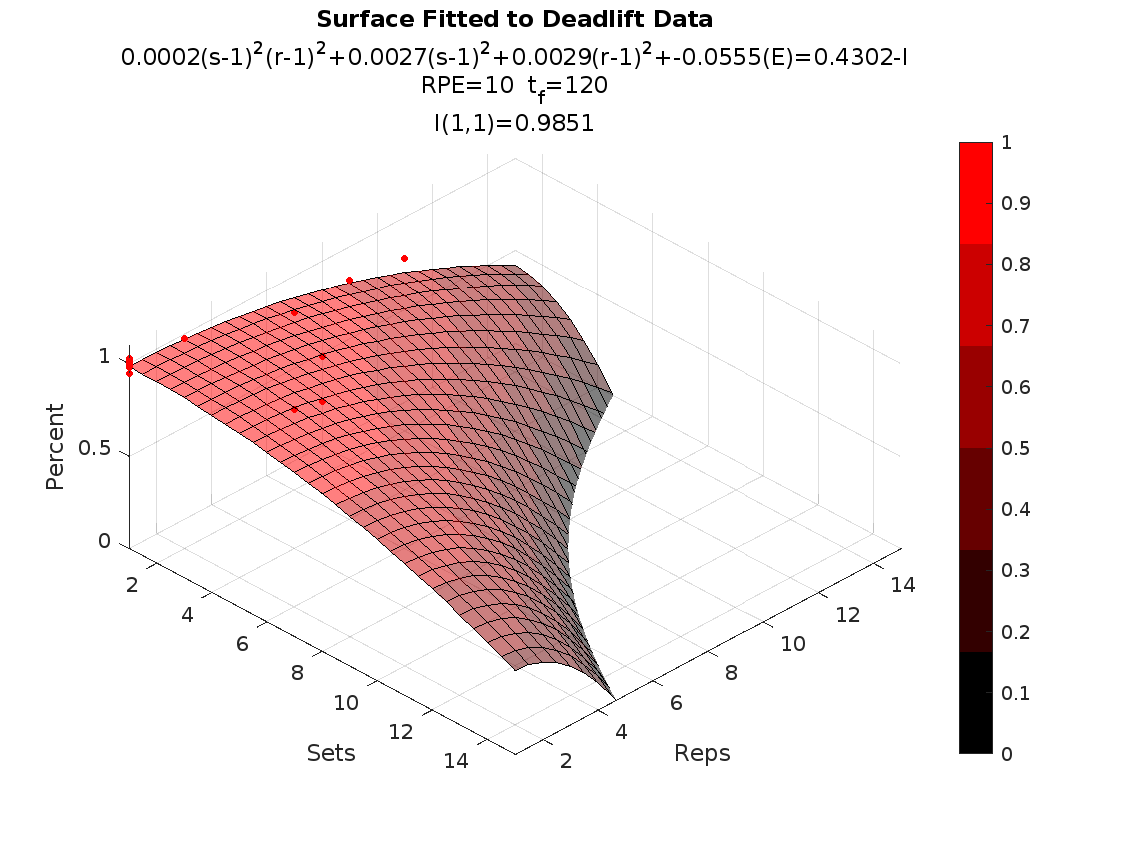
\includegraphics[width=139mm]{DeadliftSurface/10.png} \\
    \end{tabular}
    \caption{The potential surface fitted to deadlift data at various effort levels.}
    \label{tab:DeadliftPotentialSurfaceAcrossEffort}
\end{table}

Many of the relationships discussed in section \ref{sec:PotentialSurfaceIntuitiveRelationshipsBetweenVariables} are concerned with volume. To give some intuition for volume, the graphs shown in table \ref{tab:DeadliftVolumeAcrossEffort} are the result of solving the potential surface for $I$ and substituting it in equation \ref{eq:IntensityBasedVolumeEquation}.

\begin{table}[]
    \centering
    \begin{tabular}{c|c}
        RPE & Volume Graph \\%& Volume Across Intensities \\
        \hline \\
        
        5 &
        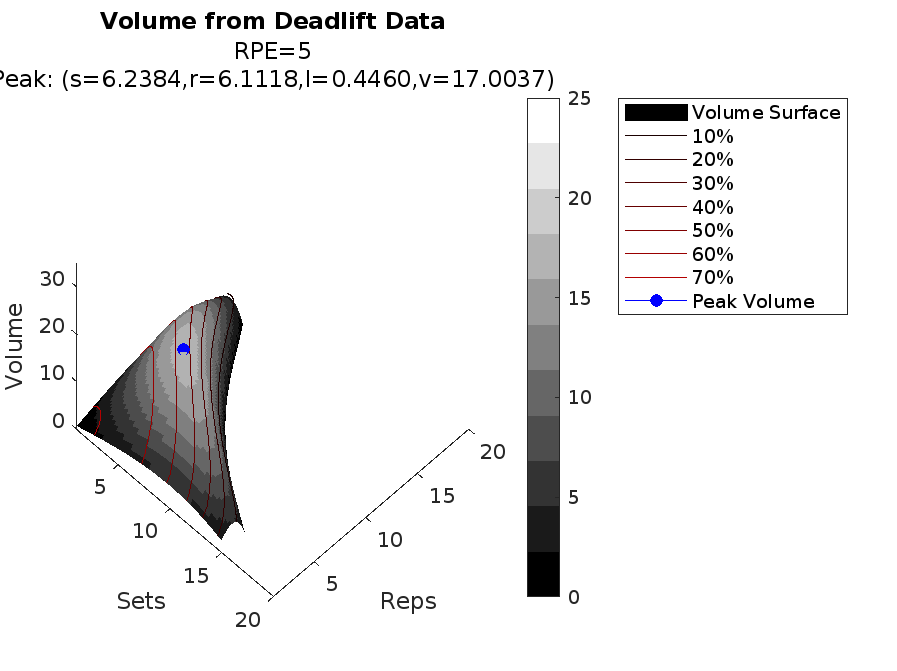
\includegraphics[width=139mm]{DeadliftVolume/5-1.png} \\%&  
        %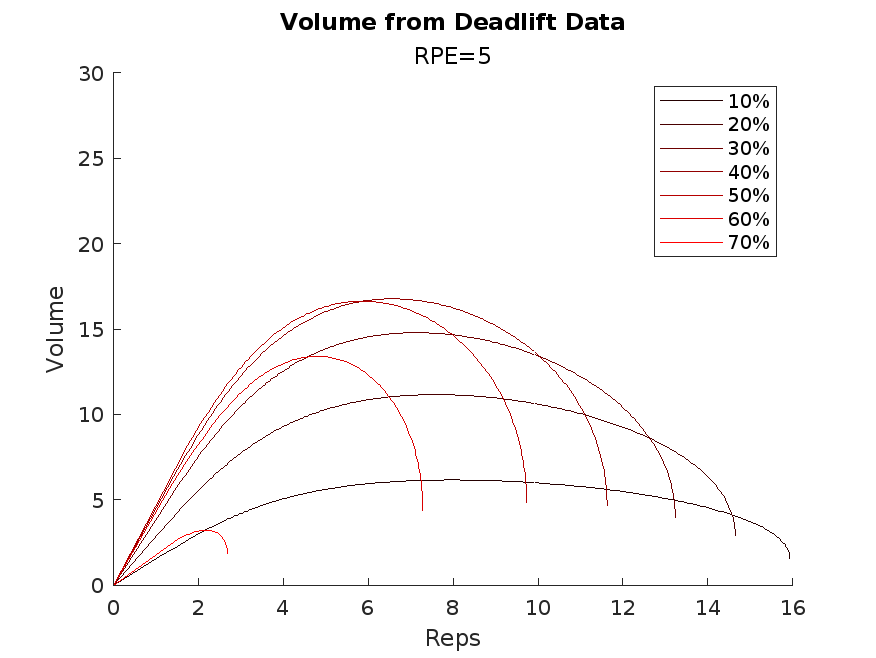
\includegraphics[width=76mm]{DeadliftVolume/5-2.png} \\
        
        %8 & 
        %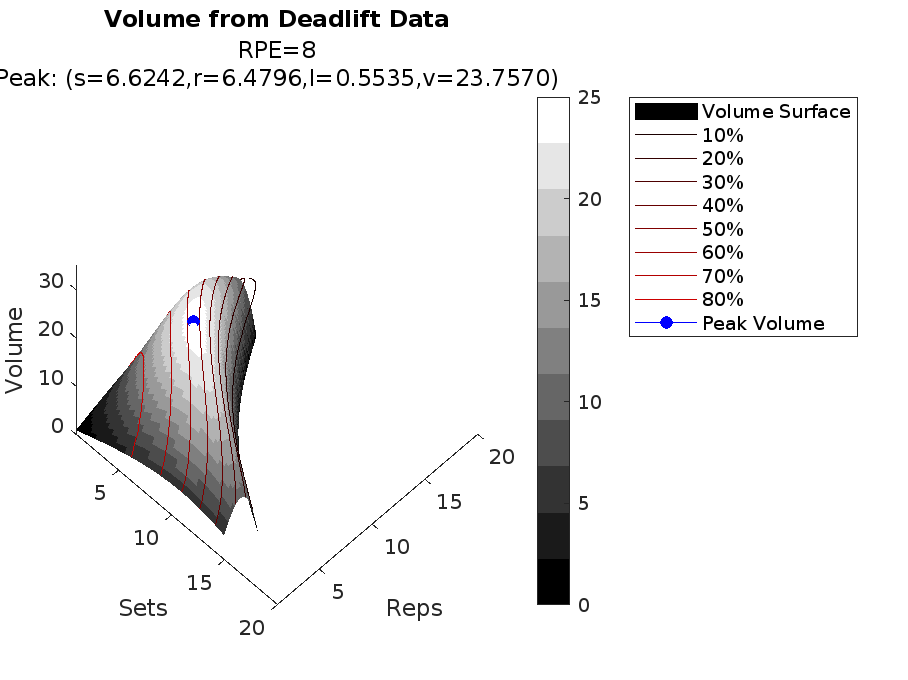
\includegraphics[width=90mm]{DeadliftVolume/8-1.png} \\%&
        %%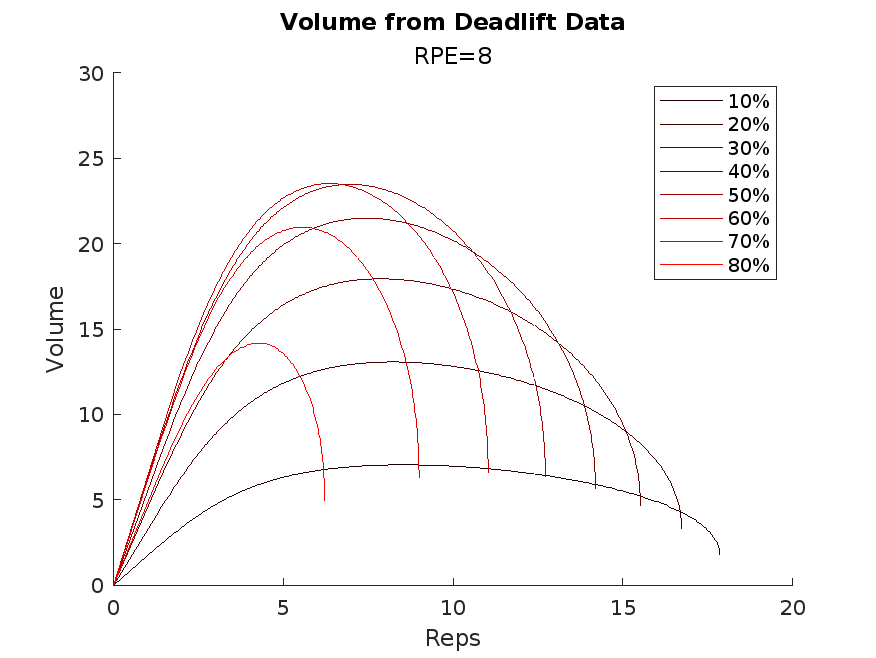
\includegraphics[width=76mm]{DeadliftVolume/8-2.png} \\
        
        10 &
        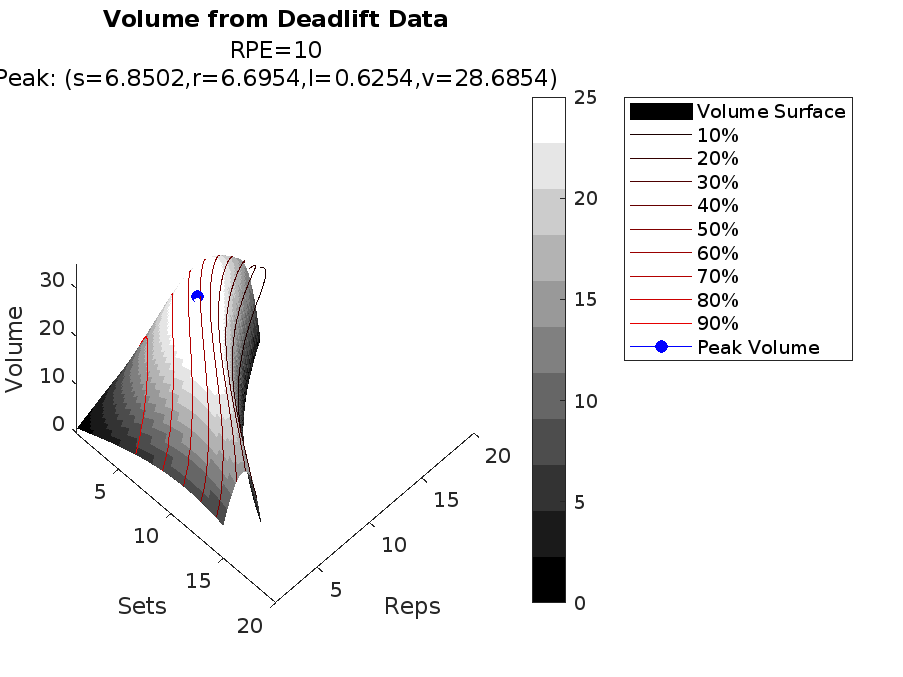
\includegraphics[width=139mm]{DeadliftVolume/10-1.png} \\%&
        %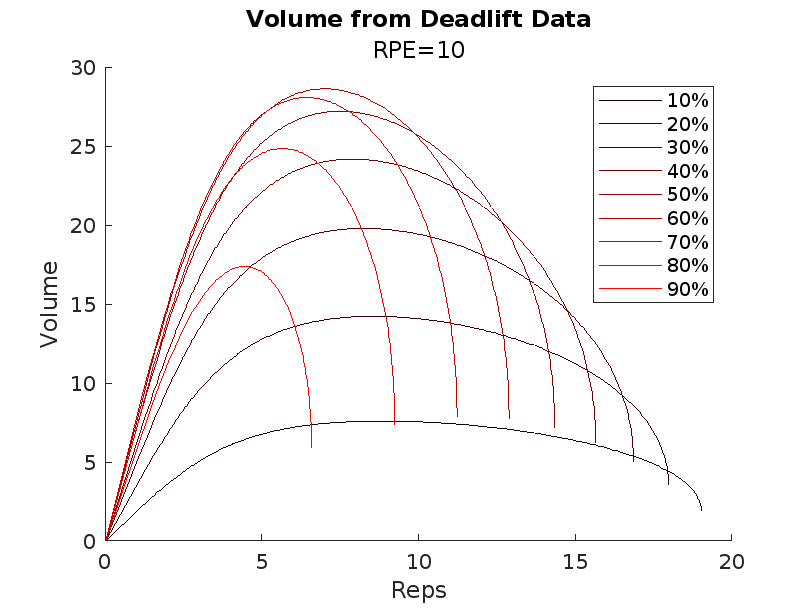
\includegraphics[width=76mm]{DeadliftVolume/10-2.png} \\
    \end{tabular}
    \caption{The volume equation from deadlift data at various effort levels. Volume was scaled linearly by $l_{1RM}$, making the vertical axis just $srI$. Note how there is a clear peak in volume as well as a ridge where volume rapidly decreases after crossing.}
    \label{tab:DeadliftVolumeAcrossEffort}
\end{table}


\section{Analysis: Proving Volume Increases With Weight Until a Peak Is Reached}
\label{sec:PotentialSurfaceVolumePeak}

It needs to be shown that, given a constant effort, volume increases with weight until a peak is reached at which point volume decreases. Analytically, this translates to finding the critical points and concavity of the volume equation. After solving equation \ref{eq:PotentialSurfaceEquation} for $s$ and substituting it in equation \ref{eq:IntensityBasedVolumeEquation}, equation \ref{eq:SetsSubedInVolume} is created and the process of finding critical points can be started. For simplicity, the volume equation will be scaled by $l_{1RM}$, removing its presence on the right hand side of the equation. The first and second partial derivatives of $v$ with respect to $I$ will also be needed.

\begin{equation}
    \label{eq:SetsSubedInVolume}
    v(r,I,E)=rI\left( \left( \frac{d-I-c(r-1)^2-\epsilon E}{a(r-1)^2+b} \right)^\frac{1}{2} +1 \right)
\end{equation}
\begin{equation}
    \label{eq:VolumeIPartialDerivative}
    \frac{\partial v}{\partial I} = 
    r+
    r\left( a(r-1)^2+b \right)^{-\frac{1}{2}} 
    \left( d-I-c(r-1)^2-\epsilon E \right)^\frac{1}{2}
    \left(
        1-\frac{I}{2}\left( d-I-c(r-1)^2-\epsilon E \right)^{-\frac{3}{2}}
    \right)
\end{equation}
\begin{equation}
    \label{eq:VolumeISecondPartialDerivative}
    \frac{\partial v'}{\partial I}=
    -r\left( a(r-1)^2+b \right)^{-\frac{1}{2}}
    \left( d-I-c(r-1)^2-\epsilon E \right)^{-\frac{1}{2}}
    \left(
        1+\frac{I}{4}\left( d-I-c(r-1)^2-\epsilon E \right)^{-1}
    \right)
\end{equation}

Both $\partial_Iv$ and $\partial_{II}v$ will need to be set to $0$ and solved for. When looking at $\partial_{II}v$, in order for a maximum to occur $\partial_{II}v<0$. Looking at the parenthetical groups of $\partial_{II}v$, the first two are guaranteed to be $\ge 0$.

\begin{enumerate}
    \item $r\ge0$ from section \ref{sec:UnitsOfMeasurement}
    \item $\left( a(r-1)^2+b \right)^{-\frac{1}{2}}>0$ from section \ref{sec:UnitsOfMeasurement} and the constraints placed on $a$ and $b$ in equation \ref{eq:PotentialSurfaceEquation}
\end{enumerate}

The third parenthetical group creates a further constraint for the current problem in question, and is shown in the inequality below. This constraint guarantees that the third parenthetical group is $>0$.

\begin{equation*}
    d-I-c(r-1)^2-\epsilon E>0
\end{equation*}

Given that the first three parenthetical groups are all $>0$, the last one must also be $>0$ in order for $\partial_{II}v$ to be $<0$. The inequality from the fourth parenthetical grouping is shown below. The constraint above nicely eliminates the imaginary part of the inequality.

\begin{equation*}
    I<\frac{4}{3}\left( d-c(r-1)^2-\epsilon E \right)
\end{equation*}

Before moving on, it is worth exploring what the above inequality has to say. As $r$ increases the range over which a maximum can occur in $I$ decreases. This may seem counter intuitive, but when considered from the perspective of volume it makes more sense. At the extreme, as the number of reps continue to increase volume continues to increase, which necessitates weight decreasing, making $I$ decrease. This is important because it shows the model respects the limitations that volume presents on weight.

Given the range where a maximum can occur, a critical point still needs to be found. This is not so easily done, and requires a computational approach. Using deadlift data, figure \ref{fig:DeadliftIntensityCriticalPoints} shows where the critical points are in relation to the region where a maximum can occur. It is clear that the critical points are all within the appropriate region to guarantee a maximum occurs.

\begin{figure}
    \centering
    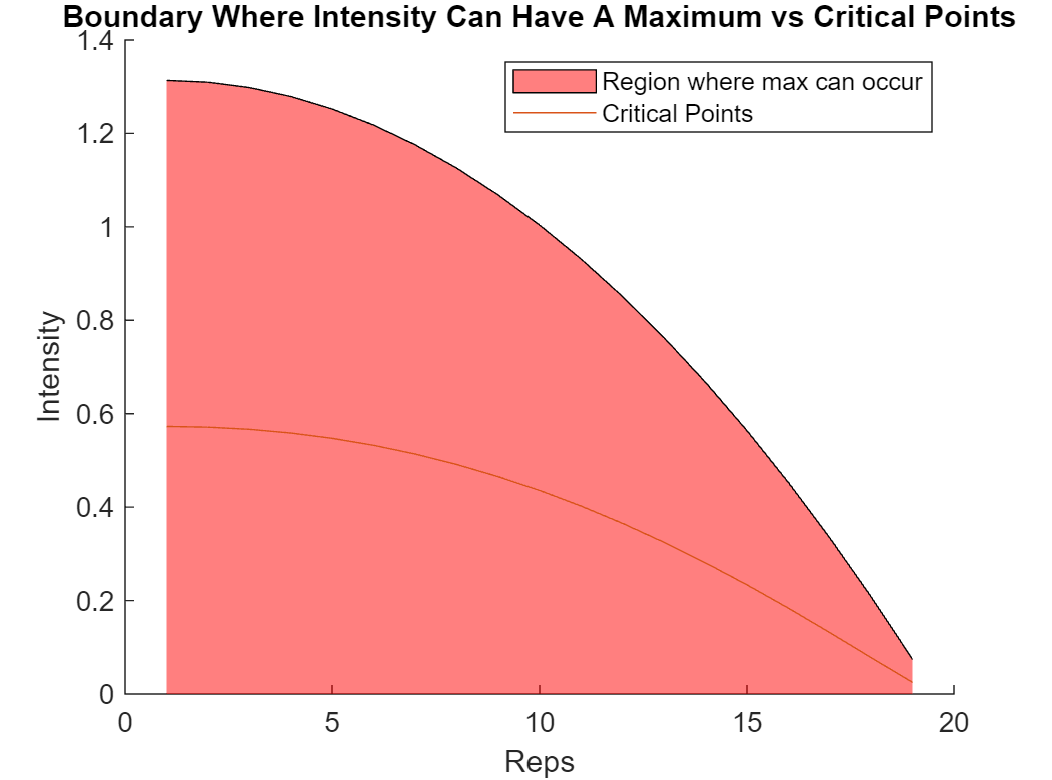
\includegraphics[width=140mm]{DeadliftConstants/IntensityCriticalPoints.png}
    \caption{Critical points for intensity from deadlift data and a time frame of 120 days with an effort of $E=5$. Note how they are all within the boundary where a maximum can occur.}
    \label{fig:DeadliftIntensityCriticalPoints}
\end{figure}

Before carrying on, it is worth mentioning that the same process used to find intensity critical points can be carried out but instead of solving equation \ref{eq:PotentialSurfaceEquation} for $s$, it can be solved for $r$. Doing this produces analogous analytical results, with $b$ and $c$ switching places along with $s$ and $r$. In order for the true peak in $I$ to be found, both approaches need to correspond to the same set of critical points. To help visualize any differences, the two sets of critical points can be plotted on top of the volume surface, as shown in figure \ref{fig:DeadliftIntensityCriticalPointsOnVolume}. From this figure, it should be clear that the two different ways to identify the peak in $I$ do not produce the same result.

\begin{figure}
    \centering
    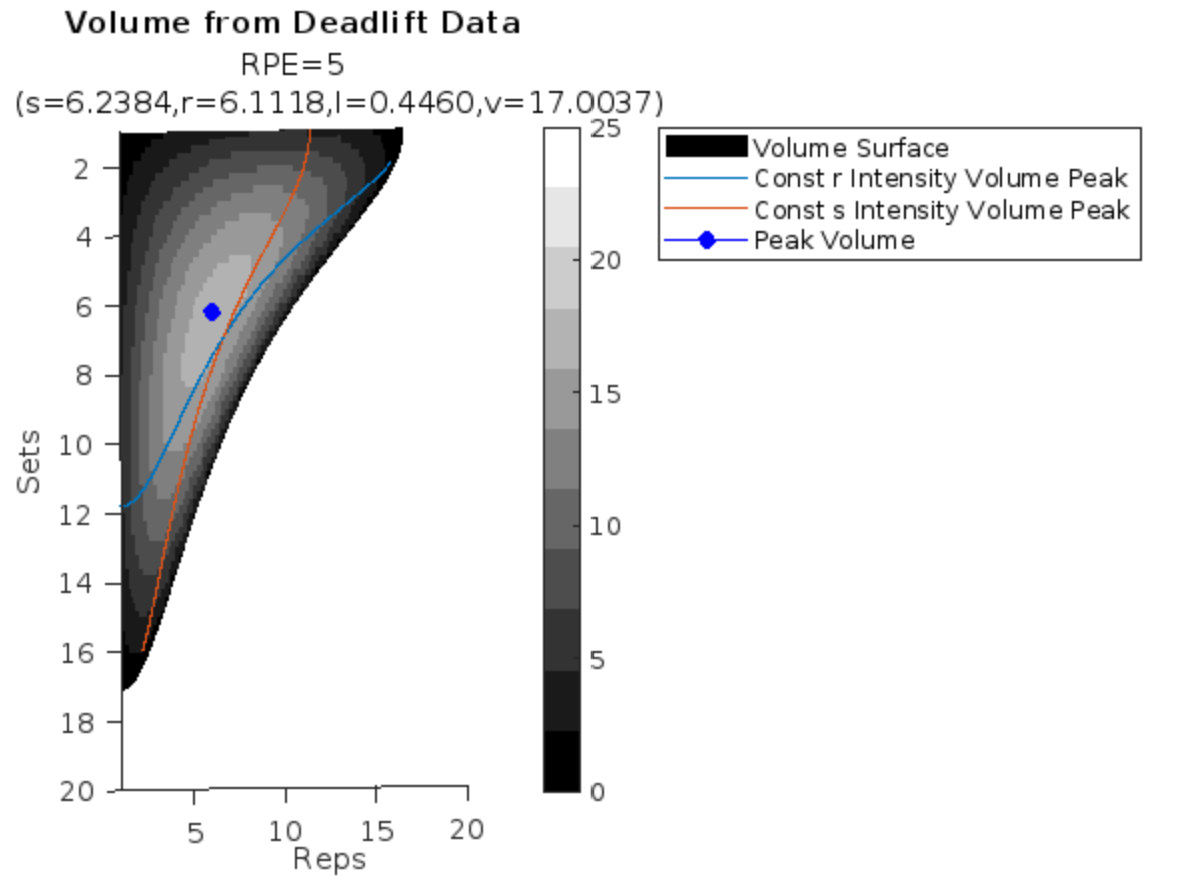
\includegraphics[width=140mm]{DeadliftConstants/IntensityCriticalPointsOnVolume.png}
    \caption{Intensity critical points graphed on the volume surface. These lines represent where intensity is maximized, in relation to constant $s$ and $r$ values.}
    \label{fig:DeadliftIntensityCriticalPointsOnVolume}
\end{figure}

The reason for the discrepancies in results can be explained by simplifying the problem to two dimensional approaches. The original three dimensional problem was reduced down to two different two dimensional problems, creating two separate ways to view the problem, and hence two different solutions. With an analytical approach failing to create consistent results, the graphs in table \ref{tab:DeadliftVolumeAcrossEffortOnlyIntensity} serve as the best proof that volume increases with effort until a peak is reached. These graphs do show some of the problems of viewing the problem from two dimensions. They show that volume does not always increase or decrease across intensity for all values of $r$. What does appear to increase across $I$ until a peak is reached is the peak volume.

\begin{table}
    \centering
    \begin{tabular}{c|c}
        RPE & Volume Across Intensities \\
        \hline
        
        5 &
        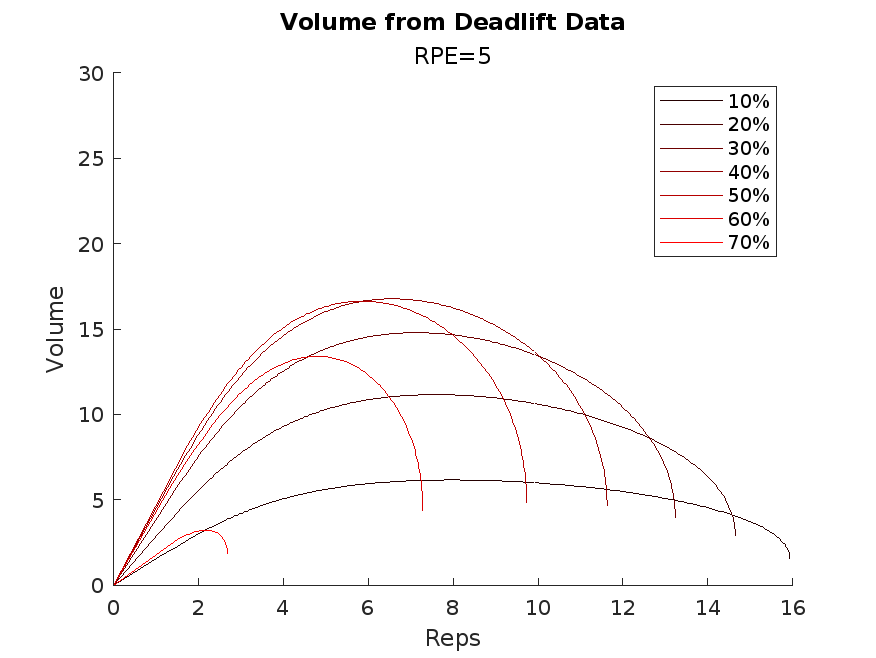
\includegraphics[width=140mm]{DeadliftVolume/5-2.png} \\
        
        %8 &
        %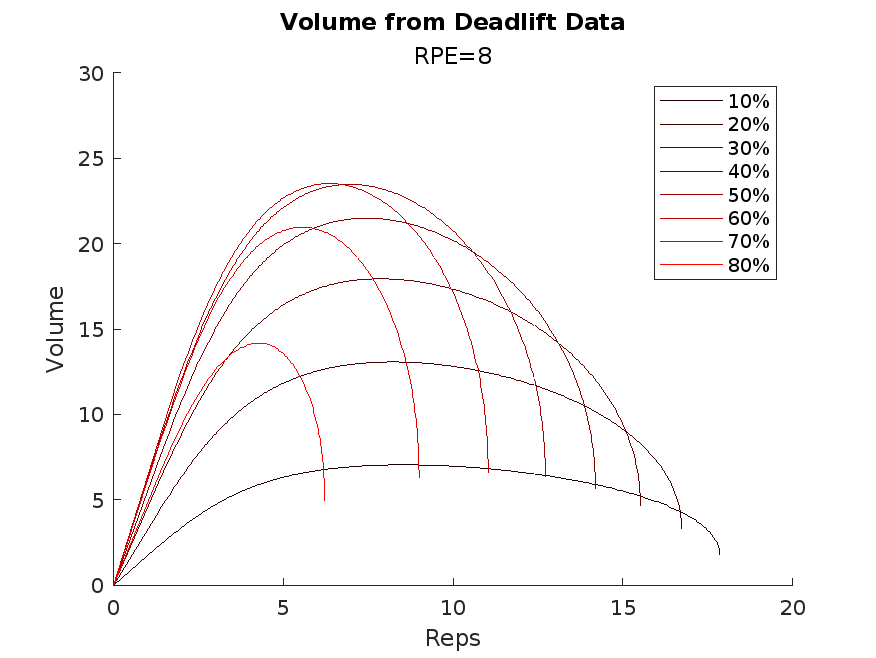
\includegraphics[width=76mm]{DeadliftVolume/8-2.png} \\
        
        10 &
        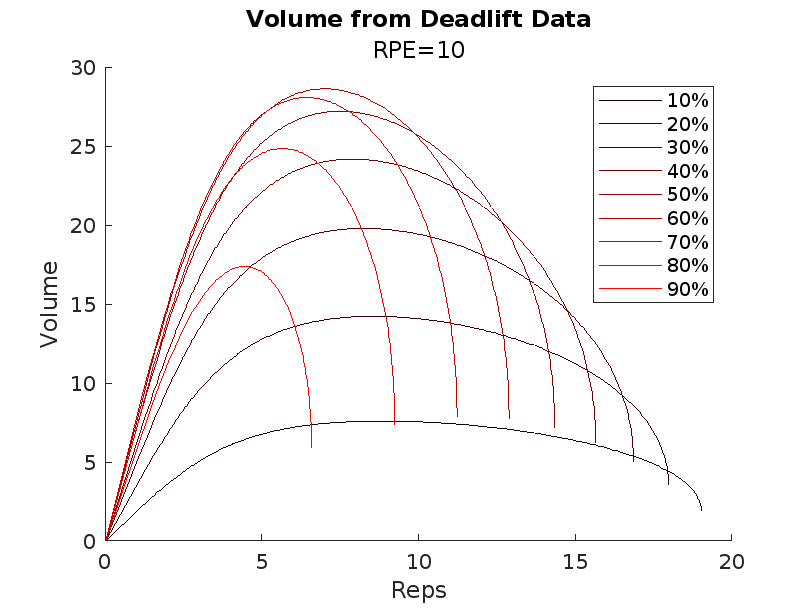
\includegraphics[width=140mm]{DeadliftVolume/10-2.png} \\
    \end{tabular}
    \caption{The same volume equation from table \ref{tab:DeadliftVolumeAcrossEffort} but only graphed across different intensities. Again, the vertical axis scaled by $l_{1RM}$. The intensity lines on the graphs in table \ref{tab:DeadliftVolumeAcrossEffort} correspond to the same intensity lines on these graphs.}
    \label{tab:DeadliftVolumeAcrossEffortOnlyIntensity}
\end{table}

%\begin{equation}
%    \label{eq:IntensitySubedInVolume}
%    v(s,r,E)=sr\left( d-a(s-1)^2(r-1)^2-b(s-1)^2-c(r-1)^2-\epsilon E \right)
%\end{equation}
%
%Finding each partial derivative of equation \ref{eq:IntensitySubedInVolume} is required. Effort is constant, making it unnecessary to find it's partial derivative.
%
%\begin{equation}
%    \label{eq:VolumeSPartialDerivative}
%    \begin{split}
%        \frac{\partial v}{\partial s}=&
%        \frac{\partial}{\partial s}sr\left( d-a(s-1)^2(r-1)^2-b(s-1)^2-c(r-1)^2 -\epsilon E \right) \\
%        =& rd-r\epsilon E-cr(r-1)^2-r\left( a(r-1)^2+b \right)\left( 3s^2-4s+1 \right)
%    \end{split}
%\end{equation}
%\begin{equation}
%    \label{eq:VolumeRPartialDerivative}
%    \begin{split}
%        \frac{\partial v}{\partial r}=&
%        \frac{\partial}{\partial r}sr\left( d-a(s-1)^2(r-1)^2-b(s-1)^2-c(r-1)^2 -\epsilon E \right) \\
%        =& sd-s\epsilon E-bs(s-1)^2-s\left( a(s-1)^2+c \right)\left( 3r^2-4r+1 \right)
%    \end{split}
%\end{equation}
%
%It should be obvious that setting equations \ref{eq:VolumeSPartialDerivative} and \ref{eq:VolumeRPartialDerivative} equal to $0$ and solving the system of equations for $s$ and $r$ is analytically impossible. As such, a computational approach is required. In the computational approach, graphing equation \ref{eq:IntensitySubedInVolume} will replace finding the concavity and gradient descent will replace solving the system of partial derivatives to get critical points. A couple graphs from equation \ref{eq:IntensitySubedInVolume} at varying effort levels are shown in table \ref{tab:DeadliftVolumeAcrossEffort}.


%Looking at the graphs in table \ref{tab:DeadliftVolumeAcrossEffort}, there is an obvious peak in volume. This peak however is not the peak in volume that needs to be identified. This peak represents the maximal possible volume across all valid intensities, sets, and reps given a constant effort. The peak in volume that needs to be identified is across all valid sets and reps given a constant intensity and effort. Despite this, for the purpose of establishing landmark values, this peak will be solved for, which will require gradient descent as shown in equation \ref{eq:VolumePeakGradientDescent}. The graphs in table \ref{tab:DeadliftVolumeAcrossEffort} identify the peak volume.
%
%\begin{equation}
%    \label{eq:VolumePeakGradientDescent}
%    \vec{v}_{n+1}=\vec{v}_{n}+\mu\nabla v_{s}(\vec{v}_{n})=\vec{v}_{n}+\mu
%    \left[
%        \begin{matrix}
%            \frac{\partial v}{\partial s}(\vec{v}_{n}) \\
%            \frac{\partial v}{\partial r}(\vec{v}_{n})
%        \end{matrix}
%    \right]
%\end{equation}
%
%Besides having a peak, there is also a ridge where once crossed volume drops drastically. This ridge is the peak in volume that needs to be verified. In order for volume to increase with weight until a peak is reached, this ridge and any lines parallel to it on the volume surface need to each have a constant intensity. It appears that the intensity lines on the graphs in table \ref{tab:DeadliftVolumeAcrossEffort} are parallel to the ridge. If only the intensity lines are graphed, as shown in table \ref{tab:DeadliftVolumeAcrossEffortOnlyIntensity}, volume seems to reach a peak across intensities. Given this, there is reason for further investigation.
%
%\begin{table}[]
%    \centering
%    \begin{tabular}{c|c}
%        RPE & Volume Across Intensities \\
%        \hline \\
%        
%        5 &
%        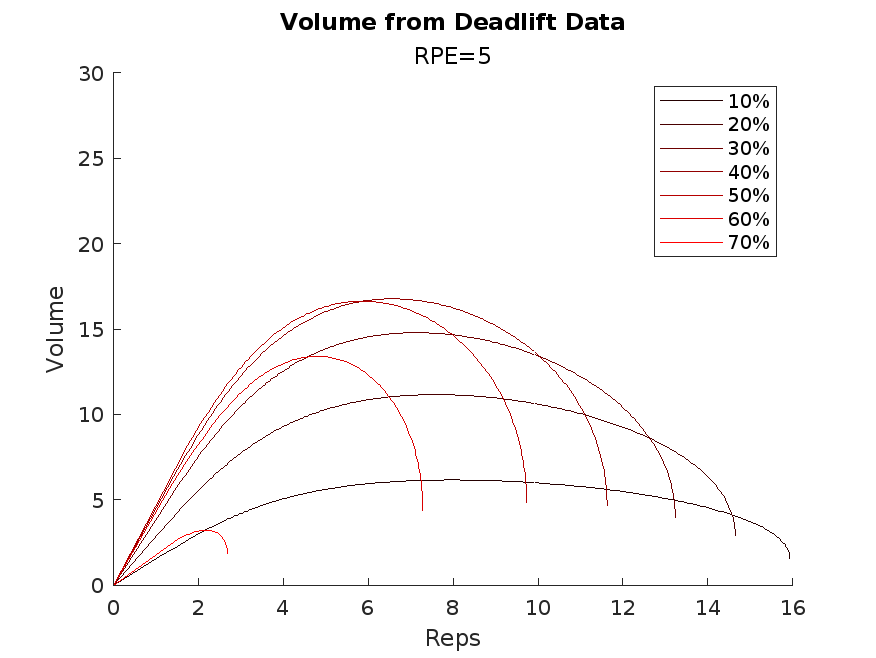
\includegraphics[width=140mm]{DeadliftVolume/5-2.png} \\
%        
%        %8 &
%        %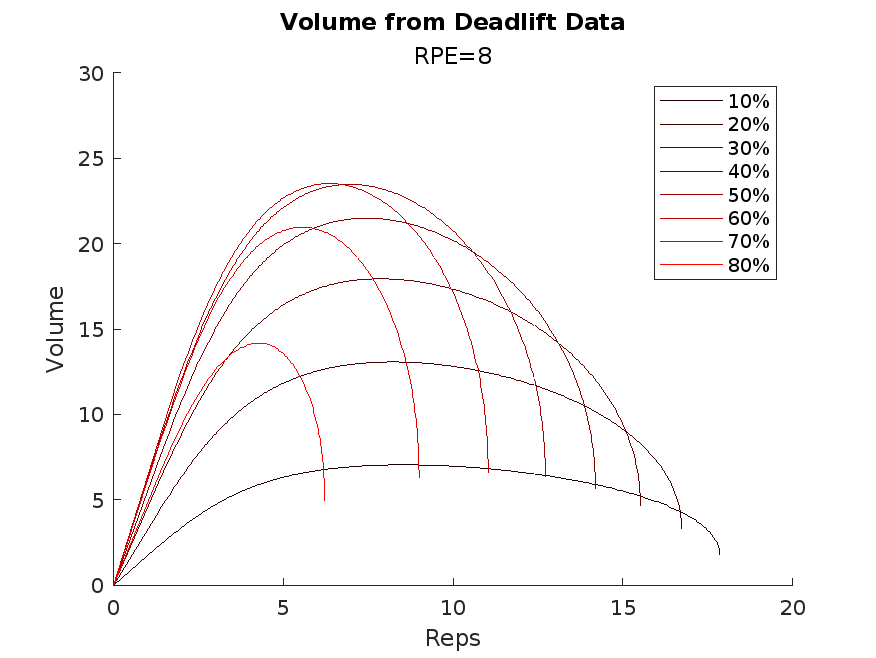
\includegraphics[width=76mm]{DeadliftVolume/8-2.png} \\
%        
%        10 &
%        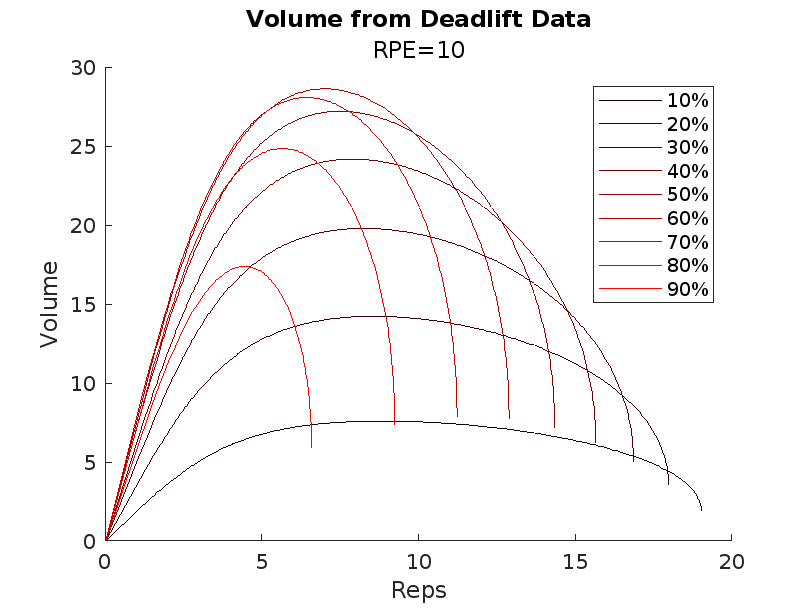
\includegraphics[width=140mm]{DeadliftVolume/10-2.png} \\
%    \end{tabular}
%    \caption{The same volume equation from table \ref{tab:DeadliftVolumeAcrossEffort} but only graphed across different intensities. The intensity lines on the graphs in table \ref{tab:DeadliftVolumeAcrossEffort} correspond to the same intensity lines on these graphs. Traveling from left to right on these graphs correspond to a clockwise rotation on the graphs in table \ref{tab:DeadliftVolumeAcrossEffort}.}
%    \label{tab:DeadliftVolumeAcrossEffortOnlyIntensity}
%\end{table}
%
%Proving the ridge and any lines parallel to it on the volume surface are all be the same intensity will be a two step process. First, the intensity values along the ridge will need to be identified to show they are constant. Once that is shown, intensities on lines parallel to the ridge will be identified to show they are constant.

%To identify the ridge one variable will be held constant and the opposite variables partial derivative will be set equal to zero and solved for. By doing this, the surface is essentially split up in an infinite set of lines, where each line is valid for a specific value of the constant variable. The peak of each line can then be identified. When all the lines peaks are stitched back together, they will all coalesce to create a new line that identifies the ridge. 

%Identifying the ridge is somewhat difficult. The first attempt held one variable constant and set the opposite variables partial derivative to $0$. Equation \ref{eq:VolumeRidgeConstS} is the result of setting the partial derivative of $v$ with respect to $r$ equal to $0$ and holding $s$ constant. Equation \ref{eq:VolumeRidgeConstR} does the same except $r$ is held constant. The idea was that the surface would essentially be sliced up in an infinite set of lines, where each line is valid for a specific value of the constant variable. The peak of each line can then be identified. When all the lines peaks are stitched back together, they will all coalesce to create a new line that identifies the ridge.
%
%\begin{subequations}
%    \begin{align}
%        \label{eq:VolumeRidgeConstS}
%        3r^2-4r+\left( 1-\frac{d-b(s-1)^2-\epsilon E}{a(s-1)^2+c} \right)&=0 \\
%        \label{eq:VolumeRidgeConstR}
%        3s^2-4s+\left( 1-\frac{d-c(r-1)^2-\epsilon E}{a(r-1)^2+b} \right)&=0
%    \end{align}
%\end{subequations}
%
%Doing this however forced a three dimensional problem into a two dimensional one, which created inconsistent results, as shown in figure \ref{fig:VolumeRidgeIdentFail}. Part of the problem is how mathematically vague the term 'ridge' is. As the work above shows, depending on how the surface is looked at 'ridge' will take different meanings.
%
%\begin{figure}
%    \centering
%    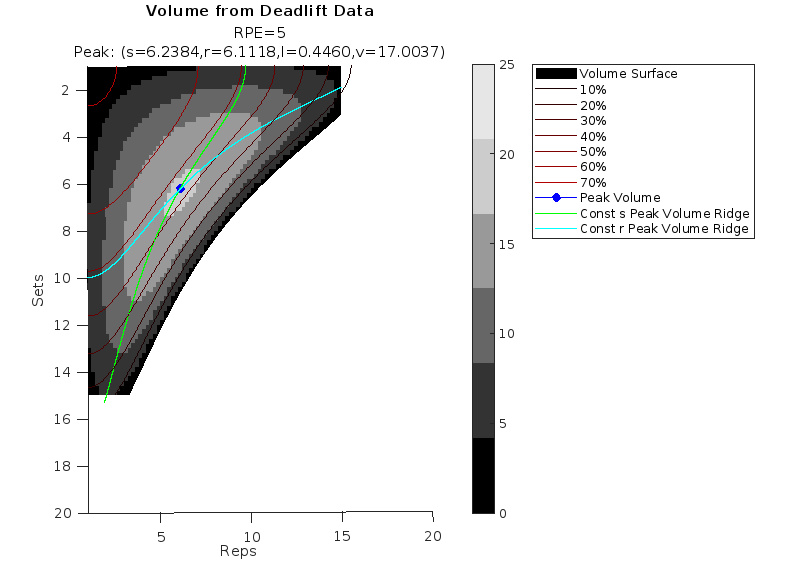
\includegraphics[width=170mm]{DeadliftVolume/FailedRidgeIdentification-2.png}
%    \caption{The first attempt at identifying the ridge. Note how the green and blue lines are not consistent with each other.}
%    \label{fig:VolumeRidgeIdentFail}
%\end{figure}
%
%While the results shown in figure \ref{fig:VolumeRidgeIdentFail} are far from perfect, some intuition can still be gained. The $50\%$ intensity line is very consistent with the two halves of the constant $s$ and constant $r$ ridge lines. This leads to the presumption that if the surface were split up into radial lines and the same process followed, a line very similar to the $50\%$ intensity line would result. While there is some basis in this approach, as equation \ref{eq:PotentialSurfaceEquation} is partially defined as an elliptic paraboloid which is circular in nature, more reasoning would be required to follow this approach.

%The second attempt to identify the ridge took a slightly different route. It started with a different volume equation, where instead of substituting equation \ref{eq:PotentialSurfaceIntensityEquation} in $v$, it substituted \ref{eq:PotentialSurfaceSetsEquation} in $v$. This allowed for the partial derivative with respect to $I$ to be taken, creating a far more direct approach than the previous attempt.

%Potentially discuss how lower intensities have more constant volume

\section{Analysis: Proving Intensity and Volume Increases With Effort}
\label{sec:PotentialSurfaceVolumeIncreasesWithEffort}

It needs to be shown that volume increases with increased effort and decreases with decreased effort. As such, the changes in $v$ relating to changes in $E$ are desired, requiring the partial derivative of equation \ref{eq:IntensitySubedInVolume} with respect to $E$.

\begin{equation}
    \label{eq:VolumeEPartialDerivative}
    \frac{\partial v}{\partial E}=
    \frac{\partial}{\partial E}srl_{1RM}\left( d-a(s-1)^2(r-1)^2-b(s-1)^2-c(r-1)^2-\epsilon E \right)=-srl_{1RM}\epsilon
\end{equation}

If $\partial_{E}v$ is always $>0$, then it can be said the function is strictly increasing, meaning volume strictly increases with increased effort. The following inequalities are given in section \ref{sec:UnitsOfMeasurement}.

\begin{equation*}
    \begin{split}
        s \ge & 1 \\
        r \in & \{ \mathbb{R}\ge 1 \} \\
        w > & 0 \\
    \end{split}
\end{equation*}

Given that $l_{1RM}$ is a weight, the following conclusion can be made given the above inequalities.

\begin{equation*}
    -srl_{1RM}\epsilon> 0 \textbf{ iff } \epsilon< 0
\end{equation*}

Therefore, it can be concluded that volume increases with increased effort \textbf{iff} $\epsilon< 0$. A similar argument can be made that proves volume decreases with decreased effort \textbf{iff} $\epsilon< 0$. If $\partial_E I$ is taken instead of $\partial_E v$, an analogous proof could be made to show that intensity increases with effort \textbf{iff} $\epsilon<0$.

Having the restriction that $\epsilon\le 0$ may seem problematic, but the $\epsilon$ value shown in table \ref{tab:DeadliftPotentialSurfaceAcrossEffort} is negative. For added reassurance, the $\epsilon$ values for three different exercises are all shown in table \ref{tab:EpsilonAcrossExercies}, and are all negative. It is clear the model is correctly identifying patterns from the training data and making volume increase with effort.

\begin{table}[h]
    \centering
    \begin{tabular}{c|c}
        Exercise & $\epsilon$ \\
        \hline
        Squat & -0.0461\\
        Bench & -0.0363\\
        Deadlift & -0.0555\\
    \end{tabular}
    \caption{The $\epsilon$ values for three different exercises. They are all negative, meaning the model is correctly making volume increase with effort.}
    \label{tab:EpsilonAcrossExercies}
\end{table}

\section{Analysis and Application: Volume Skew and Abstractly Describing Training}
\label{sec:PotentialSurfaceAbstractlyDescribingTraining}

The last intuitive relationship discussed in section \ref{sec:PotentialSurfaceIntuitiveRelationshipsBetweenVariables} is volume skew. As such, it needs to be shown that the model is capable of determining volume skew. Looking at figure \ref{fig:DeadliftIntensityCriticalPointsOnVolume} there is a clear skew towards sets with the surface reaching greater values on the set axis than the rep axis. This is consistent with the data presented in figure \ref{fig:SetsVsReps}, and is all that is needed to prove that the model can correctly identify volume skew.

Given the model can determine a volume skew, a way to represent it would be convenient. The meaning of the constants that were presented in the linear regression should be considered. The relative magnitude of constants $b$, and $c$ control how much volume can be completed favoring sets or reps respectively. As such, the ratio of $b$ to $c$, shown in equation \ref{eq:VolumeSkew}, presents itself as a way to measure volume skew. By measuring volume skew using the constants from linear regression, it is averaged across all weights and effort levels.

\begin{equation}
    \label{eq:VolumeSkew}
    v_s(b,c)=\frac{b}{c}
\end{equation}

Before continuing, the effects on equation \ref{eq:PotentialSurfaceEquation} from changes to $b$ and $c$ need to be considered. As such, equation \ref{eq:PotentialSurfaceEquation} is solved for $I$ and the partial derivative with respect to $b$ is taken. 

\begin{equation}
    \label{eq:VolumeBPartialDerivative}
    \frac{\partial I}{\partial b}=
            \frac{\partial}{\partial b} \left( d-a(s-1)^2(r-1)^2-b(s-1)^2-c(r-1)^2-\epsilon E \right)
\end{equation}

If $\partial_{b}I$ is always $\le 0$, then it can be said the function is strictly decreasing.

\begin{equation*}
    \frac{\partial}{\partial b} \left( d-a(s-1)^2(r-1)^2-b(s-1)^2-c(r-1)^2-\epsilon E \right) \le 0
\end{equation*}
\begin{equation*}
    (s-1)^2 \ge 0
\end{equation*}
\begin{equation*}
    s \ge 1
\end{equation*}

From section \ref{sec:UnitsOfMeasurement} it is guaranteed that $s\ge 1$, meaning that $I$ increases with decreases in $b$. A similar argument can be made that proves $I$ increases with decreases in $c$.

Keeping in mind how changes to $b$ and $c$ effect equation \ref{eq:PotentialSurfaceEquation}, a few initial observations can be made about equation \ref{eq:VolumeSkew}.

\begin{enumerate}
    \item If $v_s<1$ then $b<c$, which implies that the lifter favors sets for the given exercise, or has a volume skew towards sets for the given exercise.
    \item If $v_s>1$ then $b>c$, which implies that the lifter favors reps for the given exercise, or has a volume skew towards reps for the given exercise.
    \item If $v_s=1$, then the lifter has no volume skew.
    \item If $b=0$ or $c=0$ then a lifter has the maximum possible skew towards sets or reps respectively. \footnote{This idea will be explored more from volumes perspective in section \ref{sec:PotentialSurfaceUnboundedVolume}.}
\end{enumerate}

Table \ref{tab:VolumeSkewAcrossExercises} shows the constants and volume skew for three different exercises. As anticipated from the data in figure \ref{fig:SetsVsReps}, the volume skew favors sets over reps for all three exercises.

\begin{table}[h]
    \centering
    \begin{tabular}{c|c|c|c|c}
        Exercise & $b$ & $c$ & $v_s$ & Skew \\
        \hline
        Squat & $0.0001$ & $0.0020$ & $0.0272$ & Sets \\
        Bench & $0.0000$ & $0.0028$ & $0.0000$ & Sets \\
        Deadlift & $0.0027$ & $0.0029$ & $0.9495$ & Sets \\
    \end{tabular}
    \caption{Constants and the associated volume skew for three exercises.}
    \label{tab:VolumeSkewAcrossExercises}
\end{table}

The constant $a$ forms the \textit{volume base}, or the volume that should be possible no matter the magnitude of the volume skew. For example, if $b=0$ and $c>0$, then the following can be stated about the lifter and the way they perform a particular exercise:

\begin{itemize}
    \item The lifter has a volume skew towards sets because $b<c$.
    \item As the lifter leaves there normal volume skew, they should still be able to perform volume in proportion to $a$ even when $s\to 1$ and the contributions from $b$ diminish.
    \item The volume from $a$ is less than any volume that would have been present if $b>0$ because the relation between $a$ and $b$ is additive.
\end{itemize}

Having this natural representation for a volume base is important. If it was not present the model would assume when a lifter has a certain volume skew, any volume from the opposing skew would simply not be possible. In reality, this is not the case, some baseline level of volume will always be possible, even in the opposite skew.

%TODO - give examples from when linear regression was run on the data set

%Combining the above discussion about the representation of the constants with the time frame discussed in section \ref{sec:PotentialSurfaceLinearRegressionAndTimeSeriesProblems}, a new way to abstractly describe training over time is possible. Changes in $a$, $b$, and $c$ can be tracked over time to give insight as to how a lifter trained during a particular time frame. Figure \ref{fig:DeadliftConstantsOverTime} shows the constants $a$, $b$, and $c$ over time and figure \ref{fig:DeadliftVolumeSkewOverTime} shows volume skew over time. The large spike in volume skew near $30$ days is the result of the lifter utilizing AMRAP (As Many Reps As Possible) sets during training. When using AMRAP's, typically only one AMRAP set is performed. This makes for a large skew towards reps, which is evident in the volume skew graph. While presented here as an application of the model outlined so far, more will be gained from figures \ref{fig:DeadliftConstantsOverTime} and \ref{fig:DeadliftVolumeSkewOverTime} in section \ref{sec:Macrocycle}.
%
%\begin{figure}[h]
%    \centering
%    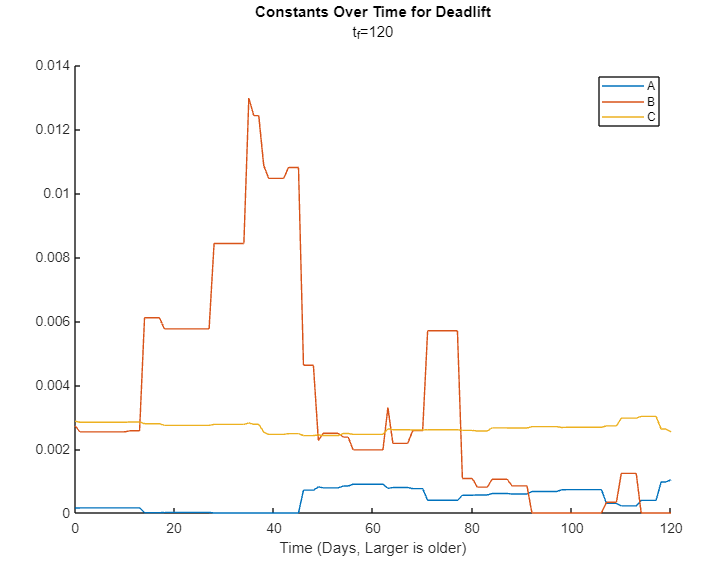
\includegraphics[width=140mm]{DeadliftConstants/abc.png}
%    \caption{The value of constants over time for deadlift when using a time frame of $120$ days. As the graph moves to the right the values are older.}
%    \label{fig:DeadliftConstantsOverTime}
%\end{figure}
%\begin{figure}[h]
%    \centering
%    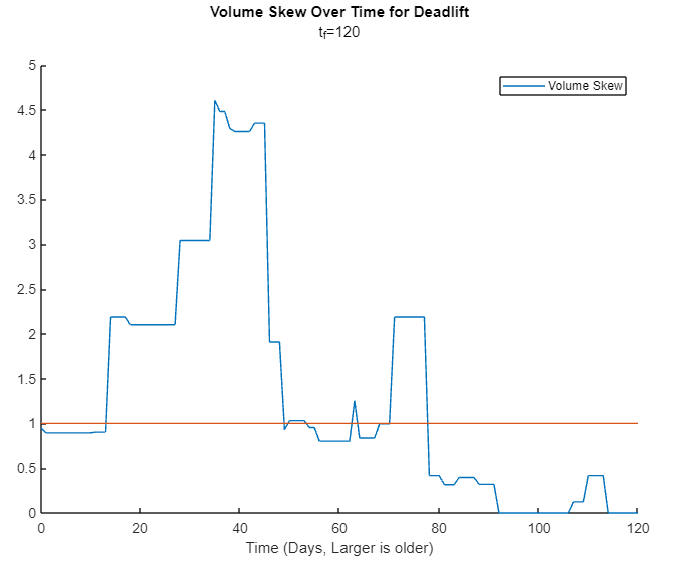
\includegraphics[width=140mm]{DeadliftConstants/VolumeSkew.png}
%    \caption{Volume skew over time for deadlift when using a time frame of $120$ days. As the graph moves to the right the values are older.}
%    \label{fig:DeadliftVolumeSkewOverTime}
%\end{figure}

\section{Analysis: Unbounded Volume}
\label{sec:PotentialSurfaceUnboundedVolume}

Unbounded volume occurs when volume continually increases. Unbounded volume is obviously not possible for a lifter to complete, and is especially problematic considering the purpose of this entire section is to establish what is possible and what is not possible. The boundary between bounded and unbounded volume needs to be found so that when this model is used in practice it works as anticipated.

If volume can be shown to have a global maximum, it can be stated that volume is bounded, or does not increase indefinitely. To prove volume has a peak requires the first partial and second partial derivative of $v$. The partial derivative with respect to $s$ was chosen. It will be discussed later what changes when the partial derivative with respect to $r$ is chosen instead.

\begin{equation}
    \label{eq:IntensitySubedInVolume}
    v(s,r,E)=sr\left( d-a(s-1)^2(r-1)^2-b(s-1)^2-c(r-1)^2-\epsilon E \right)
\end{equation}
\begin{equation}
    \label{eq:VolumeSPartialDerivative}
    \frac{\partial v}{\partial s}=rd-r\epsilon E-cr(r-1)^2-r\left( a(r-1)^2+b \right)\left( 3s^2-4s+1 \right)
\end{equation}
\begin{equation}
    \label{eq:VolumeSSecondPartialDerivative}
    \frac{\partial v'}{\partial s}=-(r)\left( a(r-1)^2+b \right)(6s-4)
\end{equation}

A global maximum occurs when $\partial_{ss} v<0$. In order for this to be the case an even number of the above parenthetical groupings need to be negative. The first parenthetical grouping is always guaranteed to be greater than $1$ from the constraints placed on $r$ in section \ref{sec:UnitsOfMeasurement}. The last parenthetical grouping will be $>0$ if $s>\frac{2}{3}$, which is again guaranteed to be true because of the constraints placed on $s$ in section \ref{sec:UnitsOfMeasurement}. This guarantees two of the three parenthetical groupings to be positive, which forces the middle parenthetical grouping to be positive for $\partial_{ss} v$ to be $<0$. The sign of $a$ changes the set of inequalities that define when the middle parenthetical group is $>0$, and hence when a maximum can occur. Table \ref{tab:BoundedVolumeRanges} shows the inequalities and ranges when volume is bounded for various values of $a$ and $b$.

Care has to be taken when $a=0$ or $b=0$, as the behavior of the inequalities is not fully captured by substituting $0$ for $a$ or $b$. A traditional limit cannot be used because inequalities are one sided, and a limit expects a continuous function. Instead, the four scenarios where $a=0$ and $b=0$ will be treated as one sided limits which will be approached from the side where the behavior is already known. By doing this, the sign can be inferred and the one sided nature of the problem can be handled. \footnote{The notation used in table \ref{tab:BoundedVolumeRanges} is as follows: given a number $x$, $x^-$ is a smaller number approaching $x$, and $x^+$ is a larger number approaching $x$. This allows for one sided analysis to be completed.} The scenarios where the root is imaginary are also troublesome. However, the same one sided analysis can be extended and used again. Looking at table \ref{tab:BoundedVolumeRanges} it should be clear how the one sided limit works as well as how the ranges over which volume is bounded respond.

\begin{table}[h]
    \centering
    \begin{tabular}{c|p{6cm}|c}
        Values for $a$ and $b$ & Inequalities & Range Where Volume is Bounded \\
        \hline

        $a>0$ and $b<0$
        &
        $r> \left(-\frac{b}{a}\right)^\frac{1}{2}+1$
        \newline
        $r< -\left(-\frac{b}{a}\right)^\frac{1}{2}+1$
        &
        $\left( r>\left| \frac{b}{a} \right|^\frac{1}{2}+1 \right) \cup \left( r< -\left| \frac{b}{a} \right|^\frac{1}{2}+1 \right)$
        \\
        \hline
        
        $a>0$ and $b=0$
        &
        $r> \left(-\frac{0^-}{a}\right)^\frac{1}{2}+1$
        \newline
        $r< -\left(-\frac{0^-}{a}\right)^\frac{1}{2}+1$
        &
        $\left( r> 1^+ \right) \cup \left( r<1^- \right)$, a.k.a. $r\ne 1$
        \\
        \hline
        
        $a>0$ and $b>0$
        &
        $r> (0+\beta i)+1$
        \newline
        $r< (-0-\beta i)+1$
        &
        $(r>1)\cup (r<1)$ a.k.a. All $r$
        \\
        \hline
        
        $a=0$ and $b>0$
        &
        $r> \left(-\frac{b}{0^+}\right)^\frac{1}{2}+1=(0+\infty i)+1$
        \newline
        $r< -\left(-\frac{b}{0^+}\right)^\frac{1}{2}+1=(-0-\infty i)+1$
        &
        $(r>1)\cup (r<1)$ a.k.a. All $r$
        \\
        \hline
        
        $a<0$ and $b>0$
        &
        $r< \left(-\frac{b}{a}\right)^\frac{1}{2}+1$
        \newline
        $r> -\left(-\frac{b}{a}\right)^\frac{1}{2}+1$
        &
        $-\left| \frac{b}{a} \right|^\frac{1}{2}+1 < r< \left| \frac{b}{a} \right|^\frac{1}{2}+1$
        \\
        \hline
        
        $a<0$ and $b=0$
        &
        $r< \left(-\frac{0^+}{a}\right)^\frac{1}{2}+1$
        \newline
        $r> -\left(-\frac{0^+}{a}\right)^\frac{1}{2}+1$
        &
        $1^- < r< 1^+$, a.k.a. Never
        \\
        \hline
        
        $a<0$ and $b<0$
        &
        $r< (0+\beta i)+1$
        \newline
        $r> (-0-\beta i)+1$
        &
        $1<r<1$ a.k.a. Never
        \\
        \hline
        
        $a=0$ and $b<0$
        &
        $r< \left(-\frac{b}{0^-}\right)^\frac{1}{2}+1=(0+\infty i)+1$
        \newline
        $r> -\left(-\frac{b}{0^-}\right)^\frac{1}{2}+1=(-0-\infty i)+1$
        &
        $1<r<1$ a.k.a. Never
        \\
    \end{tabular}
    \caption{Various values for $a$ and $b$ as well as there resulting ranges where volume is bounded.}
    \label{tab:BoundedVolumeRanges}
\end{table}

Given the ranges where a maximum could occur, a critical point is still needs to be found, which will require setting $\partial_sv$ equal to $0$. After algebraic manipulation, equation \ref{eq:VolumeRidgeConstR} is generated.
%Using the quadratic formula and substituting $\alpha_s$ in place of the fraction for ease of writing, the following points are generated as critical points.

%the equation below is generated.
\begin{equation}
    \label{eq:VolumeRidgeConstR}
    3s^2-4s+\left( 1-\frac{d-c(r-1)^2-\epsilon E}{a(r-1)^2-b} \right)=0
\end{equation}

 Using the quadratic formula and substituting $\alpha_s$ in place of the fraction for ease of writing, the following points are generated as critical points.
 
\begin{equation*}
    s=\frac{2\pm \sqrt{1+3\alpha_s}}{3}
\end{equation*}

From here the determinant can be used to show where critical points well occur.

\begin{enumerate}
    \item $\alpha_s < -\frac{1}{3}$: No critical points
    \item $\alpha_s = -\frac{1}{3}$: Indeterminate critical point
    \item $\alpha_s > -\frac{1}{3}$: Two critical points
\end{enumerate}

Given the above scenarios for critical points, only option $(3)$ is of interest. As shown below, if $\alpha_s> -\frac{1}{3}$ one critical point is generated on either side of $s=\frac{2}{3}$, the exact $s$ boundary where $\partial_{ss} v$ changes sign. Again, $\partial_{ss} v$ needs to $<0$ for a maximum to be found, requiring the parenthetical relating to $s$ in $\partial_{ss} v$ to be $>0$. This further narrows down the critical points to only include the one that is $>\frac{2}{3}$. It is worth mentioning that this is also the only valid critical point from the context of the problem, with $s$ being constrained to be $>1$ in section \ref{sec:UnitsOfMeasurement}.

\begin{equation*}
    s=\frac{2\pm \sqrt{1+3\left( -\frac{1}{3} \right)^+}}{3}=\frac{2\pm 0^+}{3}=\left( \frac{2}{3} \right)^-, \left( \frac{2}{3} \right)^+
\end{equation*}

Given that $\alpha_s>-\frac{1}{3}$, there will be a critical point. This can now be combined with the ranges where volume is bounded as well as the context of the problem to create the following statements:

\begin{enumerate}
    \item Volume is fully bounded for all $r$ when $a,b>0$.
    \item When $a>0$ and $b=0$ volume is fully bounded for all $r\ne 1$.
    \item When $a<0$ and $b=0$ volume is never bounded.
    \item When $a=0$ and $b>0$, volume is fully bounded.
    \item When $a=0$ and $b<0$, volume is never bounded.
    \item When $a>0$ and $b<0$, volume is bounded for $r>\left| \frac{b}{a} \right|^\frac{1}{2}+1$.
    \item When $a<0$ and $b>0$, volume is bounded for $1\le r < \left| \frac{b}{a} \right|^\frac{1}{2}+1$
\end{enumerate}

This analysis only looked at sets, which was an assumption made from the very beginning when the partial derivative of $v$ was taken with respect to $s$. If instead, the partial derivative was taken with respect to $r$, an analogous process would be followed. Due to the symmetry from $\partial_sv$ and $\partial_rv$, the only differences will be $c$ replacing $b$, $\alpha_r$ replacing $\alpha_s$ and, obviously, $s$ and $r$ switching roles. This creates the following additional statements given that $\alpha_r>-\frac{1}{3}$:

\begin{enumerate}
    \setcounter{enumi}{7}
    \item Volume is fully bounded for all $s$ when $a,c>0$.
    \item When $a>0$ and $c=0$ volume is fully bounded for all $s\ne 1$.
    \item When $a<0$ and $c=0$ volume is never bounded.
    \item When $a=0$ and $c>0$, volume is fully bounded.
    \item When $a=0$ and $c<0$, volume is never bounded.
    \item When $a>0$ and $c<0$, volume is bounded for $s>\left| \frac{c}{a} \right|^\frac{1}{2}+1$.
    \item When $a<0$ and $c>0$, volume is bounded for $1\le s < \left| \frac{c}{a} \right|^\frac{1}{2}+1$
\end{enumerate}

For peace of mind, figure \ref{fig:VolumeConstSRPeak} shows the peak volume identified by the above algebraic analysis. There is a peak for all $s$ and $r$ values, which means that volume is fully bounded. This also matches the statements above as $a=1.6\times 10^{-4}$, $b=2.7\times 10^{-3}$, and $c=2.9\times 10^{-3}$, which are all greater than $0$.

\begin{figure}[h]
    \centering
    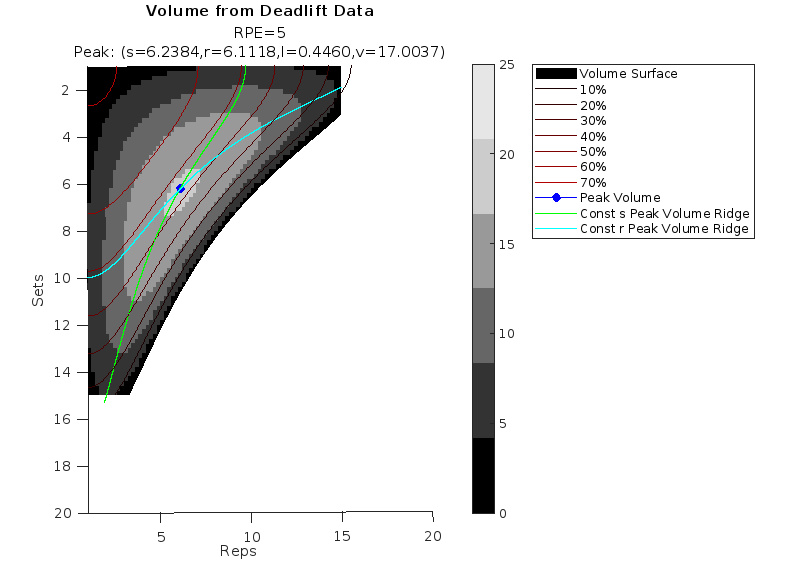
\includegraphics[width=170mm]{DeadliftVolume/FailedRidgeIdentification-2.png}
    \caption{The peak identified in volume given constant $s$ and $r$ values. This may look similar to figure \ref{fig:DeadliftIntensityCriticalPointsOnVolume} but they are two different graphs that were generated from two different approaches.}
    \label{fig:VolumeConstSRPeak}
\end{figure}

The above statements make sense in isolation, but when considered together things can contradict each other. If $a<0$, $b=0$, and $c>0$, then  statement $(3)$ states volume is never bounded, but statement $(14)$ states volume is bounded for a specific region. Again, this is the result of looking at a three dimensional problem from two dimensions, and is the same reason why the two peak volume lines in figure \ref{fig:VolumeConstSRPeak} do not coincide. While this does create some problems, the above statements are still is able to give some intuition for the problem at hand. Revisiting the example stated previously, it is saying that volume from reps is never bounded, and volume from sets is only bounded over a region. This intuition can be used to adjust training appropriately to avoid unbounded volume.

It is tempting to say the bounds in the above statements can be used in practice to limit the lifter from doing to much volume, but just because volume is bounded does not mean it is reasonable. Just because it can be proven that volume has a peak does not prove that the peak volume is attainable. This is a limitation of the model that stems from using linear regression to fit a surface to the data. Linear regression will implicitly extrapolate what amount of volume can be done given the data it has. Extrapolation is a known weakness of linear regression, making its predicted volume sometimes inaccurate.

To simplify the model, $b$ and $c$ can be limited to being $\ge 0$ so that volume will only ever be unbounded when $b=0$ or $c=0$. Not only does this remove the complexities of defining ranges over which the potential surface has bounded volume, but it makes intuitive sense to limit the model to only describing what is possible.

\section{Application: Solving for the Unknown}
\label{sec:PotentialSurfaceSolvingForTheUnknown}

With the model presented so far, one of the variables can be solved for given some combination of sets, reps, effort, or weight. This is useful because it can give a lifter information they otherwise would have guessed. Equations \ref{eq:PotentialSurfaceSetsEquation} through \ref{eq:PotentialSurfaceEffortEquation} are the potential surface solved for various variables.

\begin{subequations}
    \begin{align}
        s(r,I,E)&=
        \left( 
            \frac{
                d-I-c(r-1)^2-\epsilon E
            }{
                a(r-1)^2+b
            }
        \right)^\frac{1}{2}+1
        \label{eq:PotentialSurfaceSetsEquation}\\
        r(s,I,E)&=
        \left(
            \frac{
                d-I-b(s-1)^2-\epsilon E
            }{
                a(s-1)^2+c
            }
        \right)^\frac{1}{2}+1
        \label{eq:PotentialSurfaceRepsEquation}\\
        I(s,r,E)&=
        d-a(s-1)^2(r-1)^2-b(s-1)^2-c(r-1)^2-\epsilon E
        \label{eq:PotentialSurfaceIntensityEquation}\\
        E(s,r,I)&=
        \frac{
            d-I-a(s-1)^2(r-1)^2-b(s-1)^2-c(r-1)^2
        }{
            \epsilon
        }
        \label{eq:PotentialSurfaceEffortEquation}
    \end{align}
\end{subequations}

As an example of using the above equations, a lifter is often concerned with estimating an updated 1RM for an exercise after completing some training. Increases in weight for a lifts 1RM is a sign of progress and successful training. The model presented already estimates a users current 1RM, just in a round-about way. A 1RM will be a maximal effort lift with one set of one rep. Given these parameters, the weight lifted can be found using equation \ref{eq:PotentialSurfaceIntensityEquation}, which can just be multiplied by the weight of the lifters known 1RM to get the weight of the lifters predicted 1RM, as shown in equation \ref{eq:1RMPrediction}.

\begin{equation}
    \label{eq:1RMPrediction}
    n_{1RM}=I(s=1,r=1,E=10)l_{1RM}=l_{1RM}( d-10\epsilon )
\end{equation}

It is worth taking a step back to understand what equation \ref{eq:1RMPrediction} is saying. The new 1RM is generated from a baseline value, $d$, which increases with effort, $10\epsilon$. \footnote{Remember, $\epsilon$ needs to be $<0$ for the model to behave appropriately. This was discussed in section \ref{sec:PotentialSurfaceVolumeIncreasesWithEffort}.} This intuitively makes sense, as the more effort a lifter exerts the greater there 1RM is should be.

To test the accuracy of equation \ref{eq:1RMPrediction}, the model can be made to fit to data before a 1RM attempt and then compare the predicted 1RM to the actual 1RM. The lifter had two competitions where 1RM's were tested: the first was deadlift only and the second was a full meet. The predicted and actual 1RM's for all the exercises performed at each competition are summarized in table \ref{tab:1RMPredictedVsActual}.

\begin{table}[h]
    \centering
    \begin{tabular}{p{2cm}|p{2cm}|p{2cm}|p{2cm}|p{2cm}|p{2cm}|p{2cm}}
        Exercise & Date & Time Frame (Days) & Current Time (Days) & Predicted 1RM (lbs) & Actual 1RM (lbs) & Difference (lbs) \\
        \hline
        
        Deadlift & 5/5/2022 & $40$ & $81$ & $506$ & $520$ & $14$ \\
        Squat & 7/24/2022 & $120$ & $1$ & $415$ & $435$ & $20$ \\
        Bench & 7/24/2022 & $120$ & $1$ & $267$ & $270$ & $3$ \\
        Deadlift & 7/24/2022 & $120$ & $1$ & $511$ & $535$ & $24$ \\
    \end{tabular}
    \caption{Predicted vs actual 1RM's. All weight values are rounded to the nearest pound.}
    \label{tab:1RMPredictedVsActual}
\end{table}

The model consistently under-predicts the lifters 1RM, and the largest difference in the predicted vs actual 1RM is $24$ lbs. The smallest difference is $3$ lbs. The time frames were chosen to limit the data to only data points after $3/27/2022$, which is the date of the first successful workout after the lifter sustained an injury and took two weeks off from the gym entirely. Section \ref{sec:PotetentialSurfaceImprovingAccuracy} will work towards improving the accuracy of the predicted 1RM.

%As with section \ref{sec:PotentialSurfaceAbstractlyDescribingTraining}, a lifters 1RM can be tracked across time, providing another way to describe training over time. Figure \ref{fig:Deadlift1RMOverTime} shows the models predicted 1RM over time. Again, while presented here as an application of the model, more will be gained from figure \ref{fig:Deadlift1RMOverTime} in section \ref{sec:Macrocycle}.
%
%\begin{figure}[h]
%    \centering
%    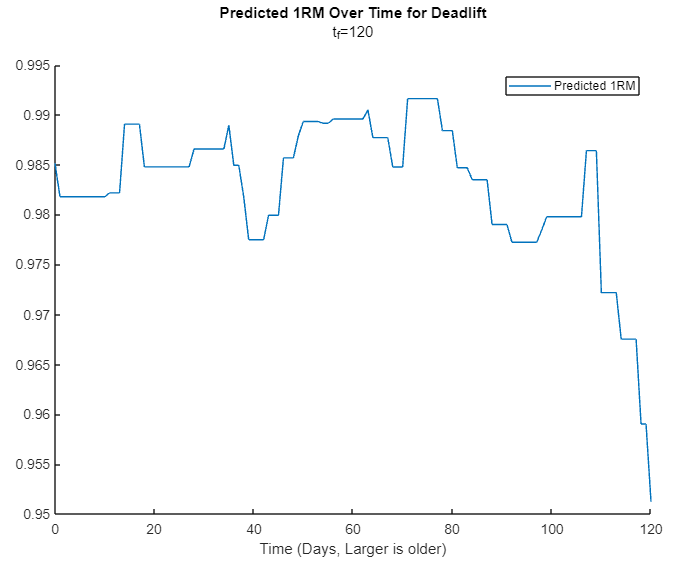
\includegraphics[width=140mm]{DeadliftConstants/pred1RM.png}
%    \caption{The models predicted 1RM over time for deadlift.}
%    \label{fig:Deadlift1RMOverTime}
%\end{figure}

\section{Improving Accuracy: Improvising for What's Not Included}
\label{sec:PotetentialSurfaceImprovingAccuracy}

Fatigue was presented in section \ref{sec:CommonTermsSection}, but until this point was not considered. This is mainly because it is not part of the data set that was used to generate the potential surface. Fatigue directly limits what can be lifted. This makes intuitive sense: a lifter that is fatigued will be tired and hence will not able to lift as much weight. This is one of the reasons why it gets harder to lift a given weight the more times it is attempted. Given this, if fatigue were to be added to the model it may look like something like equation \ref{eq:PotentialSurfaceEquationWithFatigue}, where $F$ is used to represent fatigue.

\begin{equation}
    \label{eq:PotentialSurfaceEquationWithFatigue}
    a(s-1)^2(r-1)^2+b(s-1)^2+c(r-1)^2+\epsilon E+\epsilon_2 F=d-I
\end{equation}

While fatigue cannot be represented directly by the model due to it not being part of the data, its affects should still be sought to be minimized. Within the broad category of fatigue, there two sub-types: \textit{inter-workout} and \textit{inter-exercise} fatigue. As the names suggest, inter-workout fatigue is fatigue that accumulates over the course of an entire workout, and inter-exercise fatigue is fatigue that accumulates over the course of a single exercise. When a lifter switches exercises fatigue drops depending on the amount of similarity between the exercises. If two exercises are similar more fatigue will carry over between them, increasing both the perceived inter-workout fatigue as well as the inter-exercise fatigue on the second exercise. On some occasions this is purposeful, and is used as a way to increase stimulus while keeping intensity low.

It should be obvious that effects from inter-workout fatigue cannot be minimized, as this surface is only defined for a single exercise, but the effects from inter-exercise fatigue can be partially controlled for. If the same exercise is performed on the same day with different weights, then each set with a different weight can be given an 'index' to show the order that the sets occurred in.\footnote{This obviously only includes working sets. Warm up sets will not be indexed.} This order will then take the place of a fatigue measurement, and linear regression can be completed using the augmented data set. While not perfect, this works because the index increases as fatigue would increase, creating a way to test if having actual fatigue data would increase the accuracy of the model. This 'index' will be called the \textit{fatigue index} and will will start at $0$ to reflect that the first set done will have no fatigue. If the value for $\epsilon_2$ from linear regression is not near $0$ then it can be said fatigue significantly contributes to the model. Table \ref{tab:LinearRegressionConstantsWithFatigue} shows the results after completing linear regression on deadlift data with the new augmented data set. It is clear, when compared to the other constants, the $\epsilon_2$ constant is large enough to be significant.

\begin{table}[h]
    \centering
    \begin{tabular}{c|c|c|c|c|c|c}
         & $a$ & $b$ & $c$ & $d$ & $\epsilon$ & $\epsilon_2$ \\
         \hline
        With Fatigue Index & $0.0001$ & $0.0029$ & $0.0028$ & $0.4179$ & $-0.0519$ & $0.0173$ \\
        Without Fatigue Index & $0.0002$ & $0.0027$ & $0.0029$ & $0.4302$ & $-0.0555$ & - \\
    \end{tabular}
    \caption{Linear regression constants from deadlift data with and without the augmented fatigue data.}
    \label{tab:LinearRegressionConstantsWithFatigue}
\end{table}

Despite augmenting the data set and adding a new variable, much of the work outlined in sections \ref{sec:PotentialSurfaceVolumeIncreasesWithEffort}-\ref{sec:PotentialSurfaceSolvingForTheUnknown} remains unaffected, as the added fatigue term either drops out after performing differentiation or just tags along similar to the effort term. The changes to equations \ref{eq:PotentialSurfaceSetsEquation}-\ref{eq:PotentialSurfaceEffortEquation} are shown in equations \ref{eq:PotentialSurfaceSetsEquationWithFatigue}-\ref{eq:PotentialSurfaceEffortEquationWithFatigue} for convenience.

\begin{subequations}
    \begin{align}
        s(r,I,E,F)&=
        \left( 
            \frac{
                d-I-c(r-1)^2-\epsilon E-\epsilon_2 F
            }{
                a(r-1)^2+b
            }
        \right)^\frac{1}{2}+1
        \label{eq:PotentialSurfaceSetsEquationWithFatigue}\\
        r(s,I,E,F)&=
        \left(
            \frac{
                d-I-b(s-1)^2-\epsilon E-\epsilon_2 F
            }{
                a(s-1)^2+c
            }
        \right)^\frac{1}{2}+1
        \label{eq:PotentialSurfaceRepsEquationWithFatigue}\\
        I(s,r,E,F)&=
        d-a(s-1)^2(r-1)^2-b(s-1)^2-c(r-1)^2-\epsilon E-\epsilon_2 F
        \label{eq:PotentialSurfaceIntensityEquationWithFatigue}\\
        E(s,r,I,F)&=
        \frac{
            d-I-a(s-1)^2(r-1)^2-b(s-1)^2-c(r-1)^2-\epsilon_2 F
        }{
            \epsilon
        }
        \label{eq:PotentialSurfaceEffortEquationWithFatigue}\\
        F(s,r,I,E)&=
        \frac{
            d-I-a(s-1)^2(r-1)^2-b(s-1)^2-c(r-1)^2 -\epsilon E
        }{
            \epsilon_2
        }
        \label{eq:PotentialSurfaceFatigueEquation}
    \end{align}
\end{subequations}

%As equation \ref{eq:PotentialSurfaceFatigueEquation} demonstrates, the fatigue index value can also be solved for, which presents an interesting opportunity to measure how fatigued a lifter is based on there previous lifts. Through equation \ref{eq:PotentialSurfaceEffortEquationWithFatigue}, the model will be able to predict a fatigue index. This fatigue index can then be compared to the actual fatigue index, and the delta can be used to show how fatigued you are compared to what the model expects. Equation \ref{eq:}

The changes to equation \ref{eq:1RMPrediction}, as shown in equation \ref{eq:1RMPredictionWithFatigue}, are also important. With the new predicted 1RM equation, there is still a baseline value, $d$, which increases with effort, $10\epsilon$, but the baseline value now decreases with fatigue, $\epsilon_2 F$. Again, this intuitively makes sense. If a lifter is in a fatigued state, they will not be able to lift as much weight, even with high amounts of effort. Put another way: performance is effort minus fatigue.
 
\begin{equation}
    \label{eq:1RMPredictionWithFatigue}
    n_{1RM}=I(s=1,r=1,E=10,F)l_{1RM}=l_{1RM}( d-10\epsilon-\epsilon_2 F)
\end{equation}

The updated 1RM prediction equation can be compared to the old one to see which one is more accurate. Table \ref{tab:Predicted1RMWithAndWithoutFatigue} compares the estimated 1RM's between the augmented data set and the non-augmented data set. The same lifts and time frames are used as table \ref{tab:1RMPredictedVsActual}. When computing the predicted 1RM with fatigue, a fatigue index of $F=0$ was used, as a 1RM attempt is usually the first set performed to avoid any affects from fatigue.

\begin{table}[h]
    \centering
    \begin{tabular}{p{2cm}|p{2cm}|p{3cm}|p{3cm}|p{3cm}}
        Exercise &  Date & Pred. 1RM With $F$  (lbs) & Pred. 1RM Without $F$ (lbs) & Actual 1RM (lbs) \\
        \hline
        Deadlift & 5/5/2022 & $506$ & $506$ & $520$ \\
        Squat & 7/24/2022 & $417$ & $415$ & $435$ \\
        Bench & 7/24/2022 & $269$ & $267$ & $270$ \\
        Deadlift & 7/24/2022 & $514$ & $511$ & $535$ \\
    \end{tabular}
    \caption{Predicted 1RM with and without the augmented fatigue data.}
    \label{tab:Predicted1RMWithAndWithoutFatigue}
\end{table}

As shown in table \ref{tab:Predicted1RMWithAndWithoutFatigue}, when the model is augmented with the fatigue index it has either the same or greater accuracy when predicting a 1RM, especially on bench, with the model being within $1$ pound of the users actual 1RM.

The affects of $\epsilon_2$ on $I$ also need to be considered to ensure the model is appropriately responding to fatigue. As such, the changes in $I$ relating to changes in $F$ are desired, requiring the derivative of equation \ref{eq:PotentialSurfaceEffortEquationWithFatigue} with respect to $F$. 

\begin{equation}
    \label{eq:VolumeFPartialDerivative}
    \frac{\partial I}{\partial F}=\frac{\partial}{\partial F} d-a(s-1)^2(r-1)^2-b(s-1)^2-c(r-1)^2-\epsilon E-\epsilon_2 F=-\epsilon_2
\end{equation}

As stated at the start of this section, fatigue limits what can be lifted. As such, $I$ needs to decrease as $\epsilon_2$ increases, requiring $\partial_F I<0$. It should be obvious that this can only happen if $\epsilon_2>0$, meaning that intensity decreases with fatigue \textbf{iff} $\epsilon_2>0$. Given the values for $\epsilon_2$ in table \ref{tab:Epsilon2AcrossExercises}, which are all positive, it is clear the model is appropriately identifying patterns in fatigue.

\begin{table}[h]
    \centering
    \begin{tabular}{c|c}
        Exercise & $\epsilon_2$ \\
        \hline
        Squat & $0.0116$ \\
        Bench & $0.0301$ \\
        Deadlift & $0.0173$ \\
    \end{tabular}
    \caption{The $\epsilon_2$ values for three different exercises. They are all positive, meaning the model is correctly making intensity decrease with increased fatigue.}
    \label{tab:Epsilon2AcrossExercises}
\end{table}

Augmenting the data with the fatigue index clearly improved the accuracy of the model, it is still not perfect. While the fatigue index does have the same general behavior as fatigue, it is not the exact same behavior. One difference is that fatigue will accumulate across all sets, not just across sets with a different weight. If each set was given an increasing fatigue index, regardless of weight, the model would no longer be able to accurately understand sets because every exercise would be split up into a list of single sets with a certain number of reps and an incrementing fatigue index. Splitting the data points apart like this would also create dependencies between the data points, which cannot happen with linear regression. To make sure the model accurately understands the relation between sets and reps, the fatigue index was made to only increase across sets of different weight. This has the unfortunate side effect of giving the fatigue index behavior that fatigue does not have, but is necessary to keep the rest of the model consistent.

All this consideration with the fatigue index raises the question: why not just create a new data set that records fatigue? Arguably, using actual fatigue data would give better results. The problem is that fatigue is hard to measure. A simple system like RPE cannot be used because often times a lifter may by psychologically fatigued, but physically they are fine, or visa versa. As John Broz, an Olympic trainer, says, "How you feel is a lie." While John has an extreme take on the discrepancy between how a lifter feels and how they perform, there is still some level of truth to the statement. There are many cases where a lifters psychological state does not match there physical state, resulting in discrepancies between what they think they can do and what they actually do during a workout. As such, simply asking a lifter to record how fatigued they feel on a given day is not going to produce reliable data. Other methods of measuring fatigue exist\cite{MEASURING_FATIGUE}, but these methods are generally not conducive to a training environment, which is where they would need to be used to capture changes in fatigue across sets. Finding a way to reliably record fatigue data while training will remain an unanswered question.

Due to the increased accuracy of the model with the fatigue index added to the data set, the rest of the paper will continue to use this updated model, which will be called the \textit{fatigue aware potential surface}.

%This is promising, and all seems well until volume skew is considered. Looking at $b$ and $c$ in table \ref{tab:LinearRegressionConstantsWithFatigue}, it should be obvious that the volume skew shifted. The volume skew without $F$ is $0.9495$, but with $F$ it is $1.0361$. Remembering the definition of volume skew, this means volume went from favoring sets to favoring reps. Looking at the graph from the raw data in figure \ref{fig:SetsVsReps} it should be clear the the model should favor sets, not reps.

%\section{Time Frame Considerations}
%\label{sec:PotentialSurfaceTimeFrameConsiderations}


\chapter{
    Time Frame
    \\
    \large{Fine Tuning The Model}
}
\label{sec:TimeFrame}

Section \ref{sec:PotentialSurfaceLinearRegressionAndTimeSeriesProblems} introduced the notion of a time frame, or a window of time over which data is selected to use for linear regression. This is important because it allows the model to track changes over time. The natural question then becomes how long should the time frame be, and is what this section is concerned with.

Figure \ref{fig:Pred1RMMultipleTimeFrames} shows how the predicted 1RM changes over time with varying time frames. It should be clear that the time frame chosen has a significant impact on what predictions the model makes, and as such will need to be chosen so that it increases the accuracy of the model. This will require first defining the models accuracy, and then later using that definition to choose a time frame such that the models accuracy is maximized.

\begin{figure}[h]
    \centering
    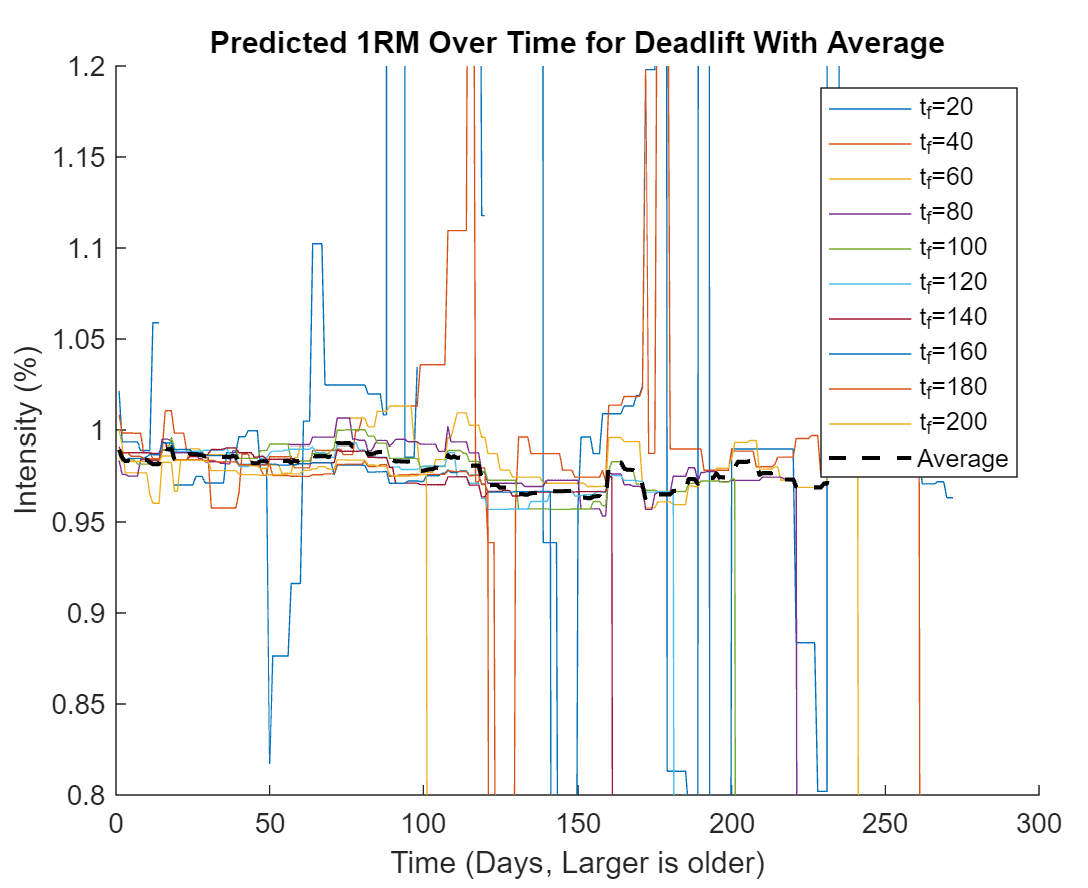
\includegraphics{DeadliftConstants/pred1RMMultipleTimeFrames.png}
    \caption{The models predicted 1RM over varying time frames. The large spikes and dips are from the model not having enough data to fit the fatigue aware potential surface to. The $20$ and $40$ time frames were excluded from calculating the average due to there erratic and inaccurate behavior.}
    \label{fig:Pred1RMMultipleTimeFrames}
\end{figure}

\section{Establishing Lose Bounds}
\label{sec:TimeFrameEstablishingLooseBounds}

The first thing to take note of from figure \ref{fig:Pred1RMMultipleTimeFrames} is the $20$ and $40$ day time frames, as they have large spikes and drops. This is the result of the model not having enough data. Given that the lifter performed deadlifts at most $2$ times a week, this creates a maximum of $11$ data points for linear regression to use over a $40$ day time frame. This is not enough data for the model to accurately predict anything. The time frame chosen needs to be large enough for the model to have enough data to reliably create predictions. With this in mind, the 1RM prediction has presented itself as a proxy to determine if the model was given enough data. If the 1RM prediction is within 'reasonable' bounds then it can be presumed that the model was given enough data to make accurate predictions. This is not an exact measurement to determine if the model has been given enough data, but is a proxy that can help avoid situations where the model was clearly not given enough data.

Looking at the larger time frames the behavior is much more stable, but at the cost of requiring more data to create any predictions. If a time frame is to large it will fail to adapt to recent changes in a lifters abilities, as it includes old data that may no longer be relevant to a lifters current capabilities. It should be clear that when considering a time frame, a balance needs to be struck so that the model has enough data to be reliable but not to much data so that it fails to capture recent changes in a lifters abilities.

\section{Accuracy: Defining State and What is Being Measured}
\label{sec:TimeFrameWhatIsBeingMeasured}

The 1RM prediction has already been introduced as a measure of accuracy in sections \ref{sec:PotentialSurfaceSolvingForTheUnknown}, \ref{sec:PotetentialSurfaceImprovingAccuracy}, and just now in section \ref{sec:TimeFrameEstablishingLooseBounds}. However, this is only a single data point from the output of the model. Accuracy can, and probably should, be considered in a much larger context. From equations \ref{eq:PotentialSurfaceSetsEquationWithFatigue}-\ref{eq:PotentialSurfaceFatigueEquation}, it can be presumed that the model can predict sets, reps, effort, intensity, and fatigue.

\begin{wrapfigure}{l}{0.55\textwidth}\centering
    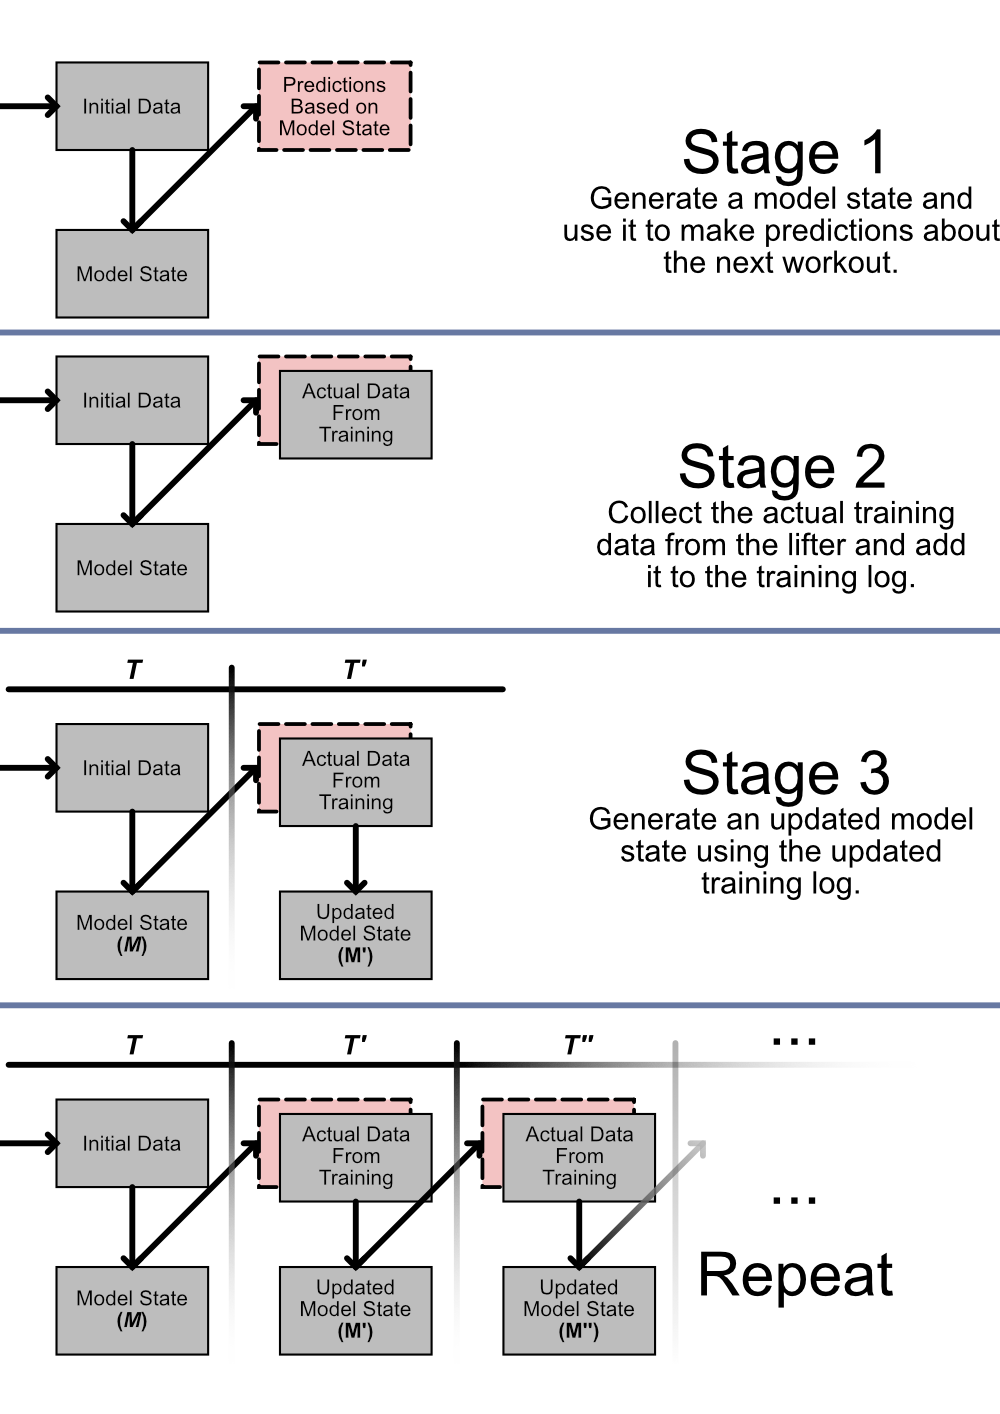
\includegraphics[width=95mm]{Diagrams/PredictionsDiagram.png}
    \caption{A diagram showing how the model makes predictions through time.}
    \label{fig:ModelPredictionsDiagram}
\end{wrapfigure}

Before any discussion about measuring accuracy, it is worth describing how the model predicts values. If the model is predicting a value for the current day, then it will use historical data that is within the selected time frame, $t_i\in\{ t_t=t_0, t_t+1=t_0+1, \dots, t_0+t_f \}$, to create a prediction. Given this specific set of historical data, the model will have a certain state, called the \textit{model state}, which is defined by the set of all constants produced from linear regression, as shown in equation \ref{eq:ModelState}. This definition makes the model state specific to the subset of historical data used, hence the $T$ subscripts, and means that the state of the model will change with any changes to the time frame. This is consistent with the observations made from figure \ref{fig:Pred1RMMultipleTimeFrames}.

\begin{equation}
    \label{eq:ModelState}
    M\in \{ a_{T}, b_{T}, c_{T}, \epsilon_{T}, \epsilon_{2,T} \}
\end{equation}

Once the actual data for a given day is added to the data set, any discrepancies between the predicted and actual data can be used to measure accuracy. When the lifter goes to train the next time, the process can repeat itself all over again, but this time the model will use time frame $T'$ and will be in in state $M'$ because of the data that was added from the previous workout. It is through this mechanism that the model is able to change state as it moves through time, and gives it the ability to adapt to represent the lifters current abilities. Figure \ref{fig:ModelPredictionsDiagram} demonstrates this process in a graphical manner.

The above process of the model updating state as it moves through time is necessary for the model to adapt, but creates challenges when attempting to gather historical data, which can be used to do things like measure accuracy over time. Every time a prediction needs to be made for time $t_t$, the model must use the appropriate time frame to get the state of the model before the data at time $t_t$ was added. Calculating the models state is a non-trivial process, and having to repeat it for every time value results in large computational overhead. Any efficiency that can be gained from calculating the models state will have significant impacts on the speed of generating historical model data.

Now that it is known how the model makes predictions, and hence how to measure accuracy, tools like the mean square error (MSE) and root mean square error (RMSE) can be used to measure accuracy from a larger context. The graphs in table \ref{tab:PredictionsVsActualConstantTimeFrame} show the actual vs predicted values for various variables using deadlift data. The reason there are not predictions for all values is because some values were to close to the end of the data set for the given time frame to make predictions, which brings up an important point: the amount of data the model needs before it can start creating predictions is dependent on the time frame chosen. This limitation will be partially removed in section \ref{sec:TimeFrameDynamicTimeFrameAnalysis}, but cannot be wholly removed because the model will always need a certain amount of data to create reliable predictions, as discussed in section \ref{sec:TimeFrameEstablishingLooseBounds}.

\begin{table}
    \centering
    \begin{tabular}{c|c}
        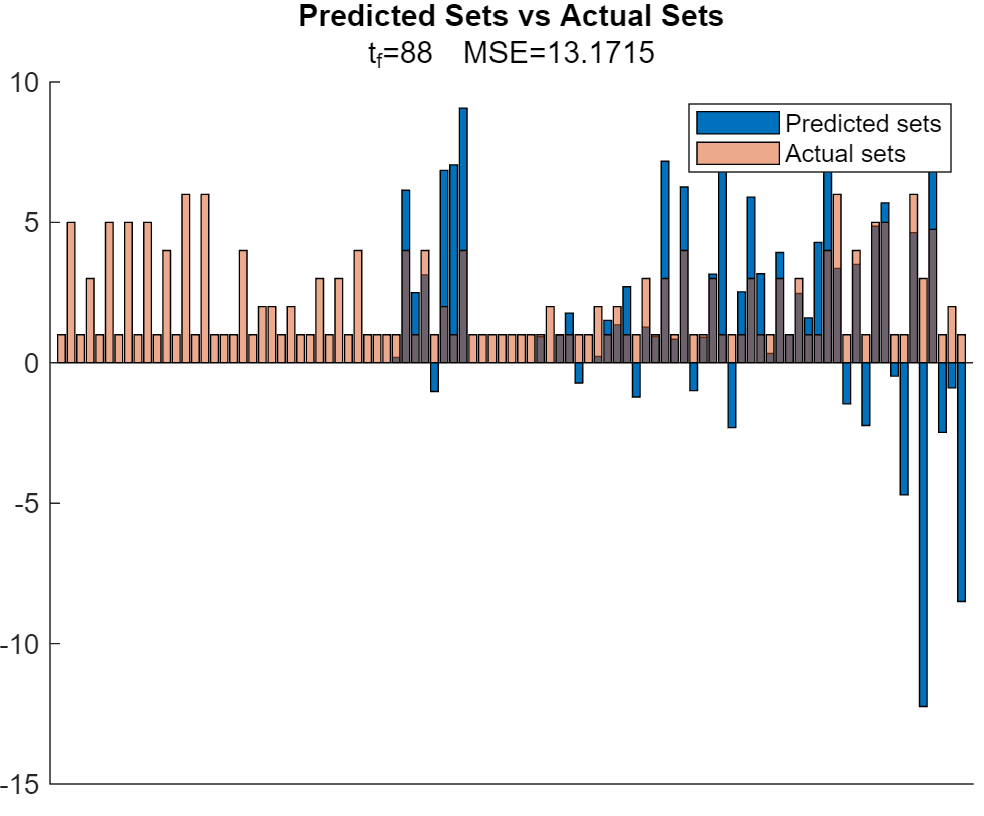
\includegraphics[width=80mm]{ActualVsPredValues/ActualVsPredSets.png} &
        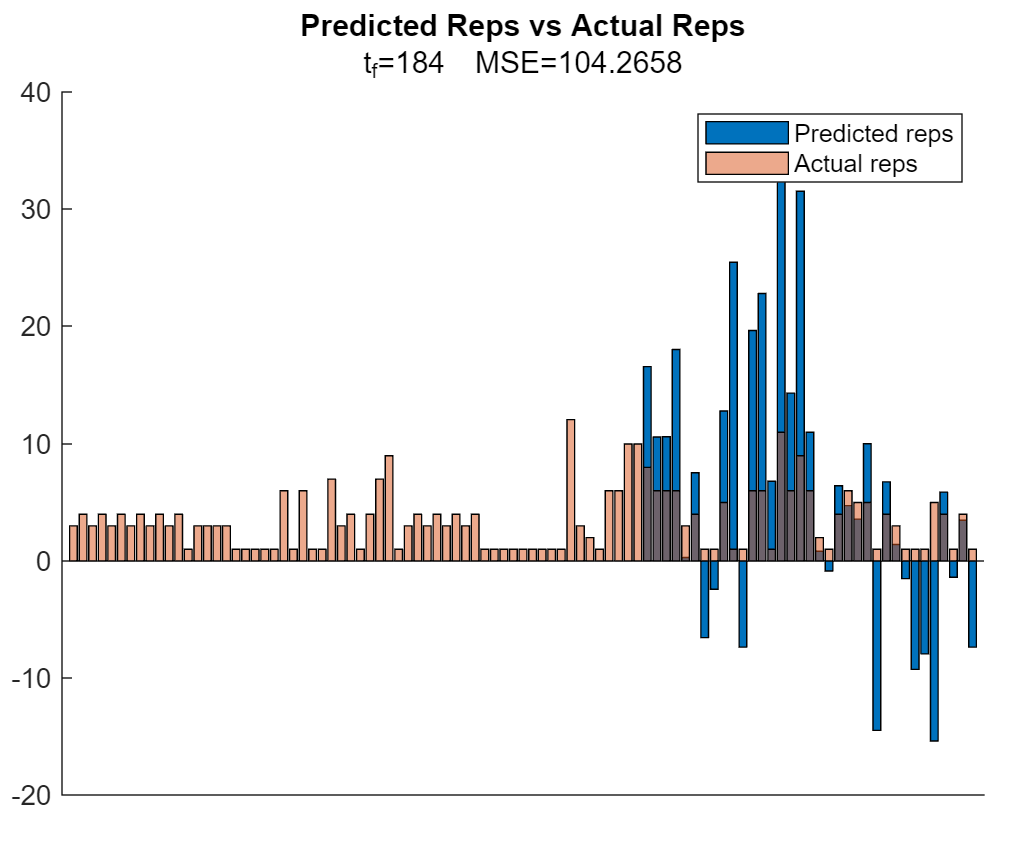
\includegraphics[width=80mm]{ActualVsPredValues/ActualVsPredReps.png}  \\
        
        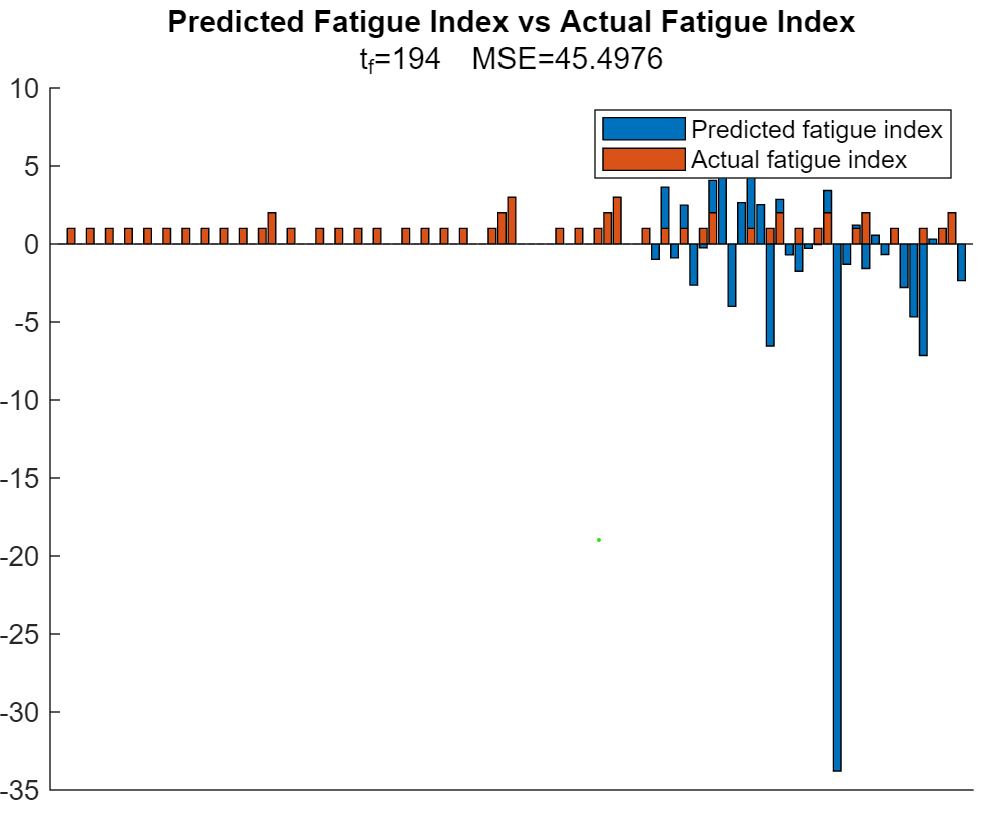
\includegraphics[width=80mm]{ActualVsPredValues/ActualVsPredFatigueIndex.png} &
        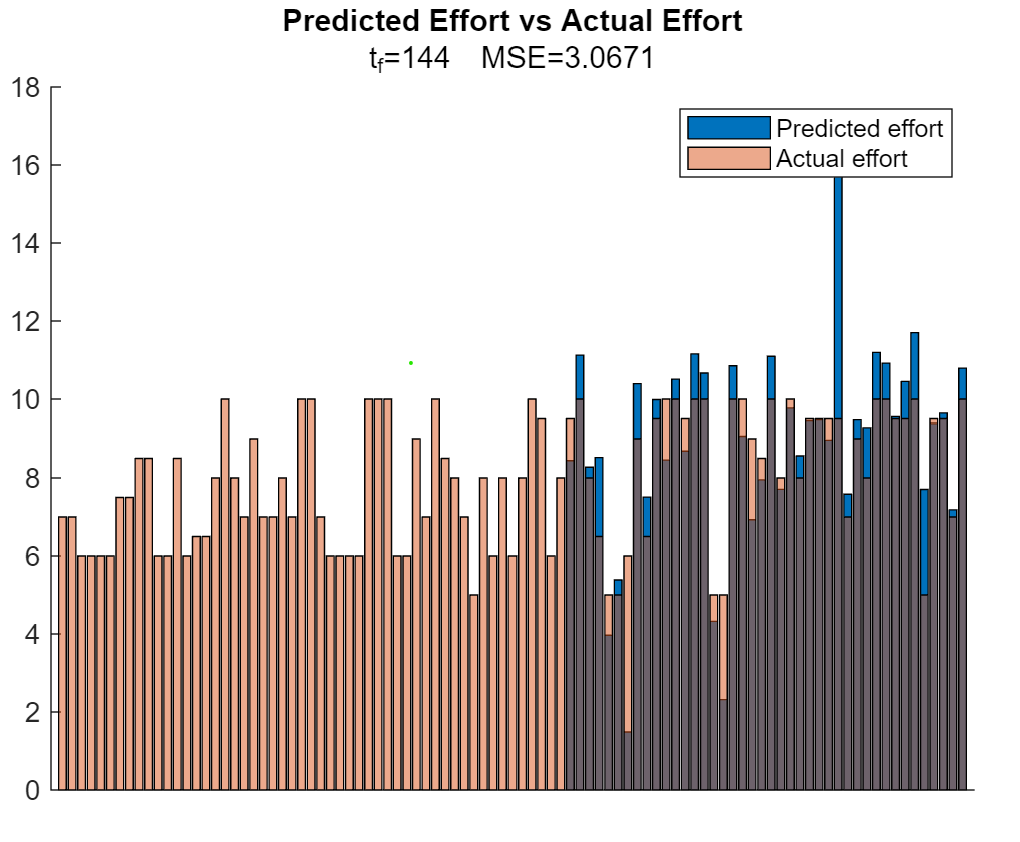
\includegraphics[width=80mm]{ActualVsPredValues/ActualVsPredEffort.png} \\
        
        \multicolumn{2}{c}{
            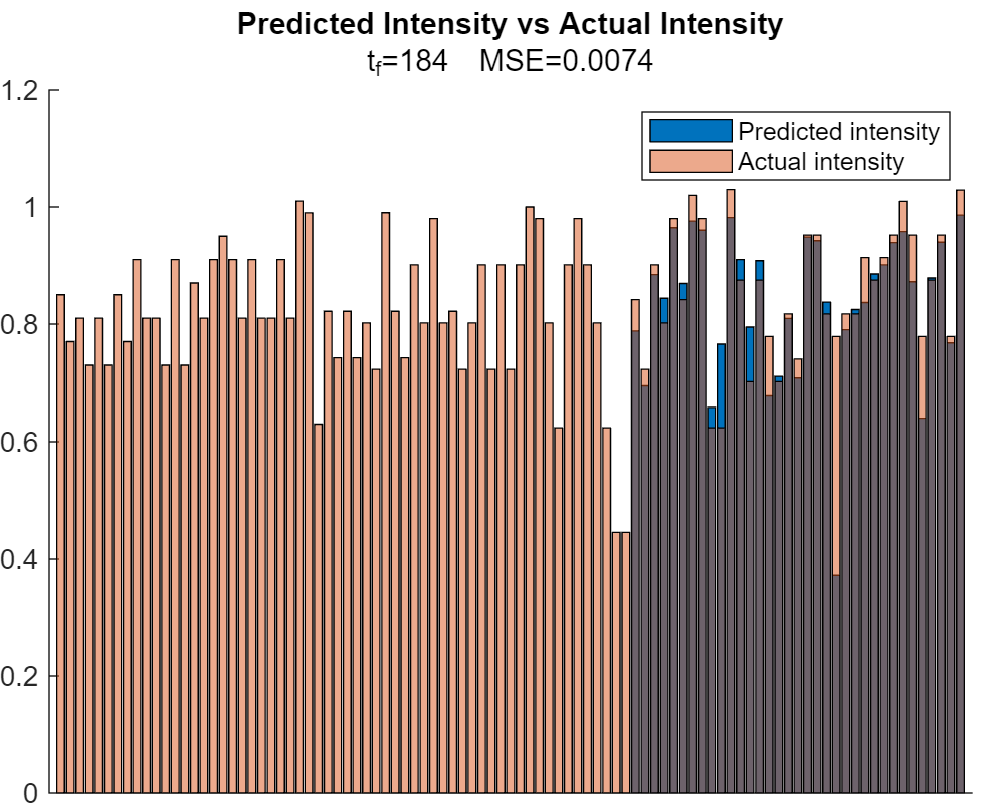
\includegraphics[width=100mm]{ActualVsPredValues/ActualVsPredIntensity.png}
        }
    \end{tabular}
    \caption{Predicted values compared to actual values for various variables using deadlift data. Sets, reps, and the fatigue index are not accurate, but effort is more accurate, and intensity is very accurate. The MSE was calculated only using data points that had a predicted value.}
    \label{tab:PredictionsVsActualConstantTimeFrame}
\end{table}

Some of the graphs from table \ref{tab:PredictionsVsActualConstantTimeFrame} may seem surprising, especially the ones relating to sets, reps, and the fatigue index. The results displayed in these graphs are highly inaccurate. The reason for this is rather simple, in section \ref{sec:PotentialSurfaceDefiningTheRelationships} the error terms that were minimized were in relation to intensity, which defined intensity as the dependent variable. Even before that however, the intuitive relationships discussed in section \ref{sec:PotentialSurfaceIntuitiveRelationshipsBetweenVariables} were all focused on how volume, effort, sets, and reps all affected intensity, which implicitly defined all of those values as independent variables and intensity the dependent variable. So, the reason for the inaccuracy in the set, rep, and fatigue index graphs are because a dependent variable was being predicted from an independent variable, which in the context of modeling does not make sense. This also explains the accuracy of the intensity graph, with the predicted intensity, on average, being within $0.74\%$ of the actual intensity. Moving forward, this means that equations \ref{eq:PotentialSurfaceSetsEquationWithFatigue}, \ref{eq:PotentialSurfaceRepsEquationWithFatigue}, \ref{eq:PotentialSurfaceEffortEquationWithFatigue}, and \ref{eq:PotentialSurfaceFatigueEquation} should all be used sparingly, and when used there results should be questioned. Of note is that equation \ref{eq:1RMPredictionWithFatigue} remains unaffected by this, and means that the 1RM predictions produced by the model should have some accuracy to them.

\section{Choosing A Time Frame: Static Time Frame Analysis}
\label{sec:TimeFrameStaticTimeFrameAnalysis}

A time frame of constant length $t_f$ can be used across all time values to generate predictions, creating a 'static time frame'. With accuracy defined and having shown how the model predicts values, the MSE of intensity across all time values can be used as a way to select a value for $t_f$ that maximizes the accuracy of the model. Figure \ref{fig:StaticTimeFrameDiagram} demonstrates the process of selecting a static time frame.

\begin{figure}[h]
    \centering
    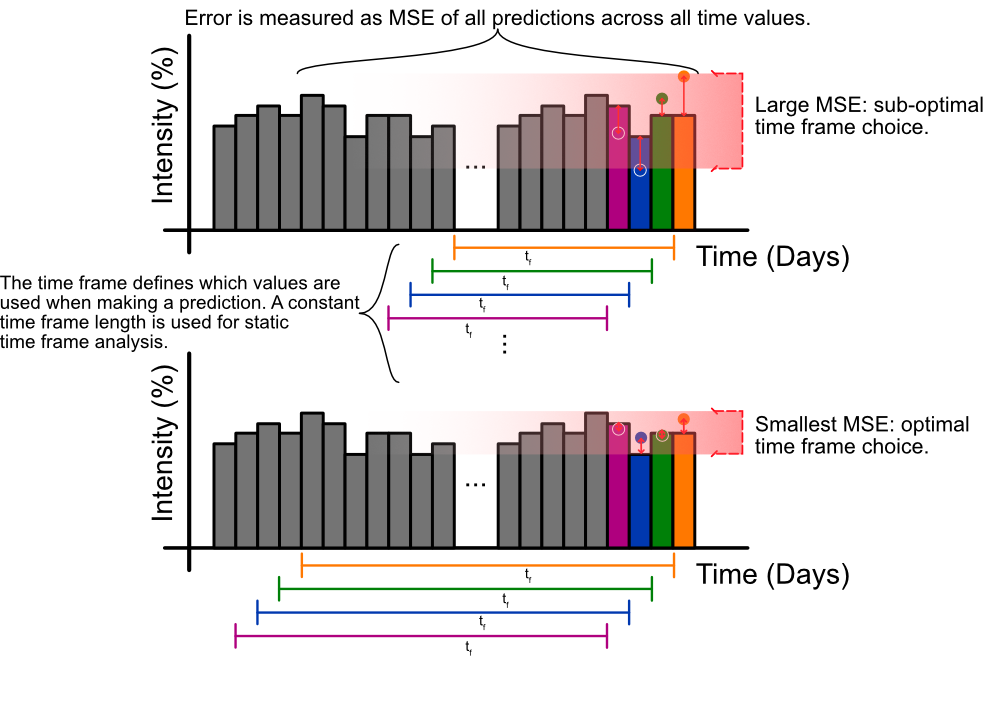
\includegraphics[width=150mm]{Diagrams/StaticTimeFrameDiagram.png}
    \caption{A diagram showing how a static time frame is calculated from the data set. Note how the predictions for all time values need to be recalculated.}
    \label{fig:StaticTimeFrameDiagram}
\end{figure}

The models accuracy will be maximized when the MSE is minimized. In order to find the global minimum MSE, all valid values of $t_f$ must be tested and there respective MSE's calculated. Equation \ref{eq:ValidTimeFrameSet} shows the set that determines all valid values for the time frame given a target time, $t_t$.

\begin{equation}
    \label{eq:ValidTimeFrameSet}
    t_f \in \{ 0, 1, \dots , \max_{t_1\dots t_n}( t )-t_t \}
\end{equation}

The algorithm shown in listing \ref{lst:StaticTimeFrameFormula} can be used to find the $t_f$ value where the MSE is minimized. Given that \texttt{modelState} runs in linear time with it's arguments, which happens because it has to sum up values across it's given time frame, this algorithm has a time complexity of $O(n^3)$. As the lifter keeps lifting and the data set grows $\max_{t_1\dots t_n}(t)$ will continually increase, eventually making an exhaustive search of all $t_f$ values infeasible. An analytical approach to finding the global minimum of the MSE would be nice, but this is not possible as the MSE error function is not a continuous function rendering any method derived from calculus useless. If historical data is needed, the time complexity gets even worse, with listing \ref{lst:HistoricalStaticTimeFrameFormula} showing the that the time complexity of getting historical data is $O(n^4)$.

% \begin{equation}
%     \sum_{t_f\in\{0,1,...,\max_{t_1...t_n}(t)\}}\left(
%         \min\left(
%             \frac{
%                 \sum_{t_{t,i}\in \{ t \; | \; t+t_{f,i}\le \max_{t_1\dots t_n}(t) \; \wedge \; t\le t_t\}}
%                 \left(
%                     intensityPred(modelState(t_{t,i+1},t_{f,i}),s_i,r_i,E_i,F_i)
%                 \right)^2
%             }{
%                 |t_{t,i}\in \{ t \; | \; t+t_{f,i}\le \max_{t_1\dots t_n}(t) \; \wedge \; t\le t_t\}|
%             }
%         \right)
%     \right)
% \end{equation}

\begin{minipage}{\linewidth}
\begin{lstlisting}[caption={The algorithm that describes how to exhaustively find a static time frame's length such that it minimizes the models error.},label={lst:StaticTimeFrameFormula},mathescape=true]
# $s$, $r$, $E$, $F$, and $t$ are all lists of there respective variables
fun staticTimeFrame$(s,r,E,F,t,t_t) \to (t_f, \varepsilon)$
    $t_{f,min}=-1$
    $\varepsilon_{min}=0$
    for each $t_{f,i}\in \{ 1, \dots, \max_{t_1\dots t_n}(t)-t_t \}$
        $\varepsilon=0$
        $\varepsilon_{cntr}=0$
        for each $t_{t,i}\in \{ t \; | \; t+t_{f,i}\le \max_{t_1\dots t_n}(t) \; \wedge \; t\ge t_t\}$
            # The $i+1$ subscript ensures the current data point, the value being
            # predicted, is not part of the model state
            $M=$modelState$(t_{t,i+1},t_{f,i})$
            $I_{pred}=$intesityPrediction$(M,s_i,r_i,E_i,F_i)$
            $\varepsilon=\varepsilon+(I_{pred}-I_{i+1})^2$
            $\varepsilon_{cntr}+=1$
        $\varepsilon/=\varepsilon_{cntr}$
        if $\varepsilon<\varepsilon_{min}$
            $\varepsilon_{min}=\varepsilon$
            $t_{f,min}=t_{f,i}$
    return $( t_{f,min}, \varepsilon )$
\end{lstlisting}
\end{minipage}

\begin{minipage}{\linewidth}
\begin{lstlisting}[caption={The algorithm that describes how to find historical static time frames.},label={lst:HistoricalStaticTimeFrameFormula},mathescape=true]
# $s$, $r$, $E$, $F$, and $t$ are all lists of there respective variables
fun historicalStaticTimeFrames$(s,r,E,F,t) \to \left( [t_{f,1},\dots,t_{f,n}], [\varepsilon_1,\dots,\varepsilon_n] \right)$
    $t_{f,min}=[0, 0, \dots]$ where $|t_{f,min}|=n$
    $\varepsilon_{min}=[0, 0, \dots]$ where $|\varepsilon_{min}|=|t|$
    for each $t_{t,i}\in \{ t \} $
        $(t_{f,min}[i], \varepsilon_{min}[i])=$staticTimeFrame$(s,r,e,F,t)$
    return $(t_{f,min},\varepsilon_{min})$
\end{lstlisting}
\end{minipage}

If the summations used in \texttt{modelState} are saved then a dynamic programming approach can be used to reduce the time complexity of \texttt{modelState} to constant time, reducing the time complexity of listing \ref{lst:StaticTimeFrameFormula} to $O(n^2)$ and listing \ref{lst:HistoricalStaticTimeFrameFormula} to $O(n^3)$. Despite the drastic improvement, these time complexities are still not usable as the data set gets larger.

Without a clear way to further optimize the static time frame algorithm presented in listing \ref{lst:StaticTimeFrameFormula}, the problem needs to be constrained. One way to do this is to only find a local minimum of the MSE. Conceptually, the approach to determine a local minimum of the MSE is not much different from whats outlined in listing \ref{lst:StaticTimeFrameFormula}. Instead of exhaustively searching the entire set of $t_f$ values, the algorithm stops when it finds a minimum. This will result in time savings as long as the MSE is not continually decreasing across the entire range of $t_f$ values.

Another approach to constrain the problem is to simply bound the time frame to always be less than a certain length and only search for a minimum MSE value within a specific range of $t_f$ values. This approach was used to create the graphs in table \ref{tab:PredictionsVsActualConstantTimeFrame}. The MSE values for all $t_f\in \{ 60, 61, ... , 200 \}$ were used, and from this set, the $t_f$ value corresponding with the smallest MSE relative to the variable being predicted was then selected to generate each graph, explaining the different time frame values shown in the table. Figure \ref{fig:MSEStaticTimeFrame} shows the MSE values for every $t_f$ value when intensity was the variable being predicted. It demonstrates the non-continuous nature of the MSE, and demonstrates the obvious fact that the first minimum is not guaranteed to be the global minimum.

\begin{figure}[h]
    \centering
    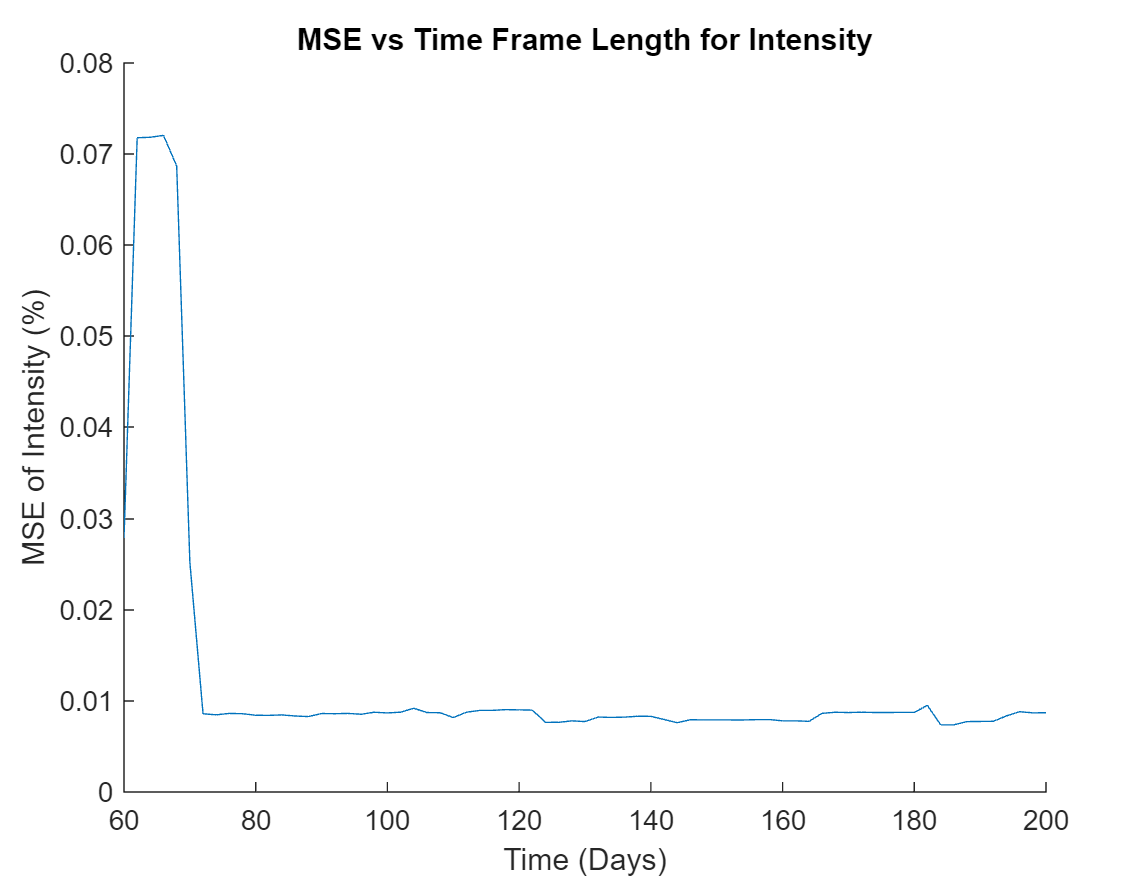
\includegraphics[width=140mm]{ActualVsPredValues/MSEvsStaticTimeFrame.png}
    \caption{The MSE over for intensity given different values of $t_f$. Note how the first minimum is not the global minimum within the context of this graph.}
    \label{fig:MSEStaticTimeFrame}
\end{figure}

Other than the obvious time complexity issues, a static time frame has other drawbacks that are more pertinent to the models behavior. In essence, the algorithm in listing \ref{lst:StaticTimeFrameFormula} will find the time frame that minimizes error across all time values greater than the target time. This results in the model finding a value for $t_f$ that minimizes error for all times greater than $t_t$, measuring accuracy in terms of the models \textit{global accuracy}. However, measuring accuracy this way violates the models efforts to adapt to the lifters current abilities. A static time frame may fail to capture changes, especially if changes are abrupt, or it may adapt to slowly, especially if the time frame is to long. If the lifters abilities change over time, then so to should the length of the time frame, thereby allowing changes in a lifters abilities to be more easily expressed.

\section{Choosing A Time Frame: Dynamic Time Frame Analysis}
\label{sec:TimeFrameDynamicTimeFrameAnalysis}

If the length of the time frame is allowed to vary over time it will give the model more freedom to adapt to the lifters current abilities. Much of the setup will remain the same from section \ref{sec:TimeFrameStaticTimeFrameAnalysis}, with equation \ref{eq:ValidTimeFrameSet} remaining valid in this section.  Figure \ref{fig:DynamicTimeFrameDiagram} demonstrates the process of selecting a dynamic time frame.

The algorithm to find a dynamic time frame is shown in listing \ref{lst:DynamicTimeFrameFormula}. The general idea of the algorithm is to select a time frame that minimizes the error of the closest data before the target time, and then that time frame can be used to predict the intensity at the target time. The main difference between the static and dynamic algorithms is the dynamic algorithm only measures accuracy in terms of the target time, and not in terms of every time before the target time. This results in the dynamic algorithm using the square error (SE) instead of the MSE to calculate accuracy for each individual target time. Once the SE is found for each target time the MSE can then be found across all target times. In essence, the dynamic time frame approach is only concerned with \textit{local accuracy}, whereas the static time frame approach is concerned with global accuracy.

\begin{figure}[h]
    \centering
    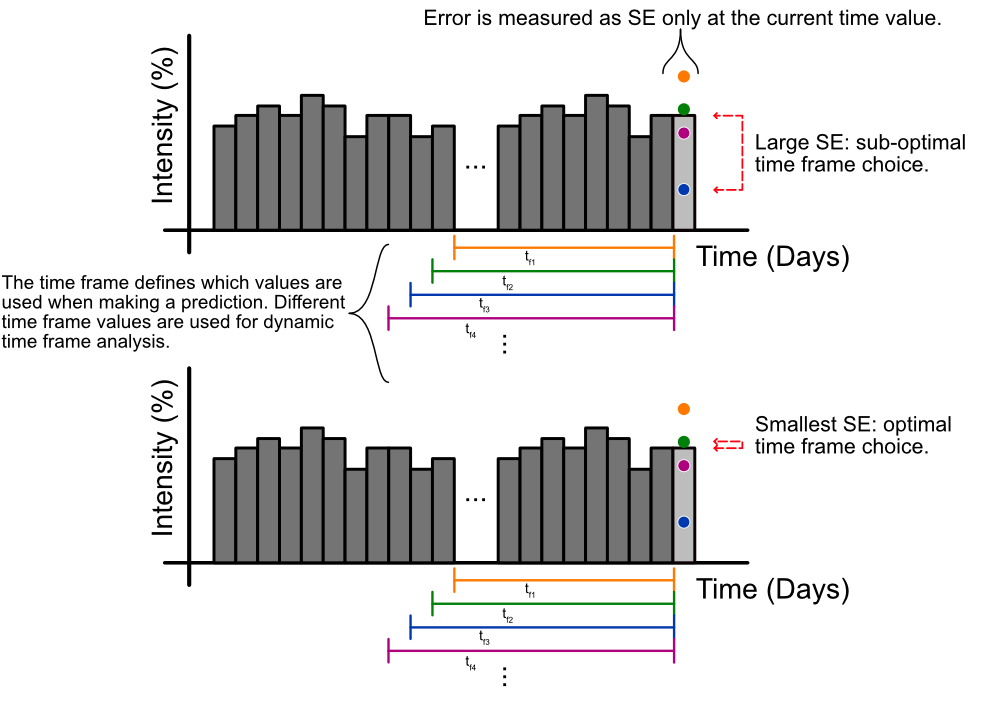
\includegraphics[width=150mm]{Diagrams/DynamicTimeFrameDiagram.png}
    \caption{A diagram showing how a dynamic time frame is calculated from the data set.}
    \label{fig:DynamicTimeFrameDiagram}
\end{figure}

A side effect of only measuring accuracy locally is an improved time complexity. The algorithm shown in listing \ref{lst:DynamicTimeFrameFormula} has a time complexity of $O(n^2)$, which is better than the $O(n^3)$ time complexity of the comparable static algorithm. This is also true for the algorithm to find historical data, with the dynamic algorithm shown in listing \ref{lst:HistoricalDynamicTimeFrameFormula} having a time complexity of $O(n^3)$. Obviously, these time complexities are still not great but it is a step in the right direction.

A dynamic programming approach similar to the one used in the static algorithm can also be used in listing \ref{lst:DynamicTimeFrameFormula} to reduce it's time complexity to $O(n)$. A linear time complexity is manageable, making the dynamic algorithm a viable way to select a time frame. This also reduces the time complexity of \ref{lst:HistoricalDynamicTimeFrameFormula} to be $O(n^2)$, which is not great, but can still be used to generate recent historical data.

Of course, only measuring accuracy locally does have some negative effects. Only measuring accuracy locally means that less information about the models performance is available when compared to the static algorithm. This is shown in the return values in listings \ref{lst:StaticTimeFrameFormula}-\ref{lst:HistoricalDynamicTimeFrameFormula}, with less information being returned from the dynamic algorithms. This is not a major concern however, as the accuracy of the model can still be assessed with the output of the dynamic algorithm.

\begin{minipage}{\linewidth}
\begin{lstlisting}[caption={The algorithm that describes how to exhaustively find a dynamic time frame's length such that it minimizes the models error.},label={lst:DynamicTimeFrameFormula},mathescape=true]
# $s$, $r$, $E$, $F$, and $t$ are all lists of there respective variables
fun dynamicTimeFrame$(s,r,E,F,t,t_t) \to \left( t_{f}, d_{iff} \right)$
    $t_{f,min}=0$
    $d_{iff,min}=\infty$
    $M_{min}=\{\}$
    for each $t_{f,i}\in \{ t_f \; | \; t_{t+1}+t_f\le \max_{t_1\dots t_n}(t) \} $
        # The $t+1$ subscript ensures the current data point, the value being
        # predicted, is not part of the model state
        $M=$modelState$(t_{t,i+1},t_{f,i})$
        $I_{pred}=$intesityPrediction$(M,s_{t+1},r_{t+1},E_{t+1},F_{t+1})$
        $d_{iff}=(I_{pred}-I_{t+1})^2$
        if $d_{iff}<d_{iff,min}$
            $\left( d_{iff,min}, t_{f,min}, M_{min} \right)=\left(  d_{iff}, t_{f,i}, M \right)$
    return $(t_{f,min},(\texttt{intensityPrediction}(M_{min},s_t,r_t,E_t,F_t)-I_t)^2)$
\end{lstlisting}
\end{minipage}

\begin{minipage}{\linewidth}
\begin{lstlisting}[caption={The algorithm that describes how to find historical dynamic time frames.},label={lst:HistoricalDynamicTimeFrameFormula},mathescape=true]
# $s$, $r$, $E$, $F$, and $t$ are all lists of there respective variables
fun historicalDynamicTimeFrames$(s,r,E,F,t) \to \left( [t_{f,1},\dots,t_{f,n}], \varepsilon \right)$
    $d_{iff}=[\infty, \infty, \dots]$ where $|d_{iff}|=|t|$
    $t_{f,min}=[0, 0, \dots]$ where $|t_{f,min}|=|t|$
    for each $t_{t,i}\in \{ t \}$
        $(t_{f,min}[i],d_{iff}[i])=$dynamicTimeFrame$(s,r,E,F,t,t_{t,i})$
    return $($
        $t_{f,min}$,
        $\texttt{sum}(
            \texttt{filter}(d_{iff},\texttt{val}!=\infty)
        )/
        \texttt{count}(
            \texttt{filter}(d_{iff},\texttt{val}!=\infty
        )$
    $)$
\end{lstlisting}
\end{minipage}

Figure \ref{fig:PredictionsVsActualDynamicTimeFrame} is the result of running the dynamic time frame algorithm on deadlift data. Note how the MSE has decreased to $0.42\%$ compared to $0.78\%$ from the static algorithm. Put another way: using a dynamic time frame the model is, on average, within $0.42\%$ of the actual intensity. Other than the increased accuracy, another thing of note is the increased range over which predictions were able to be made compared to the static time frame shown in table \ref{tab:PredictionsVsActualConstantTimeFrame}. This is because the models time frame was able to shrink when it butted up against the end of the data set in the dynamic approach, whereas in the static approach if the time frame went past the end of the data set no predictions could be made.
%and figure \ref{fig:TimeFrameAcrossTime} shows the time frame length across time

\begin{figure}[h]
    \centering
    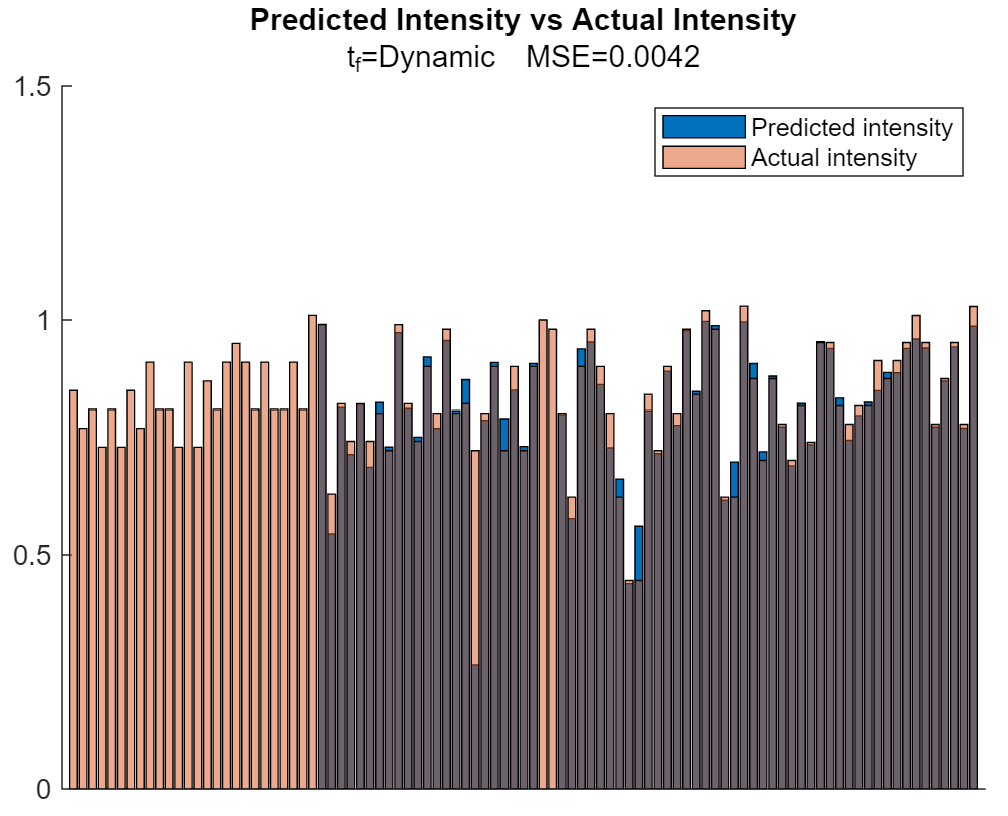
\includegraphics[width=120mm]{ActualVsPredValues/DynamicTimeFrameActualVsPredIntensity.png}
    \caption{Predicted values compared to actual values for intensity using deadlift data. Note how using the dynamic time frame extended the range of values that have predictions while still having higher accuracy.}
    \label{fig:PredictionsVsActualDynamicTimeFrame}
\end{figure}
%\begin{figure}[h]
%    \centering
%    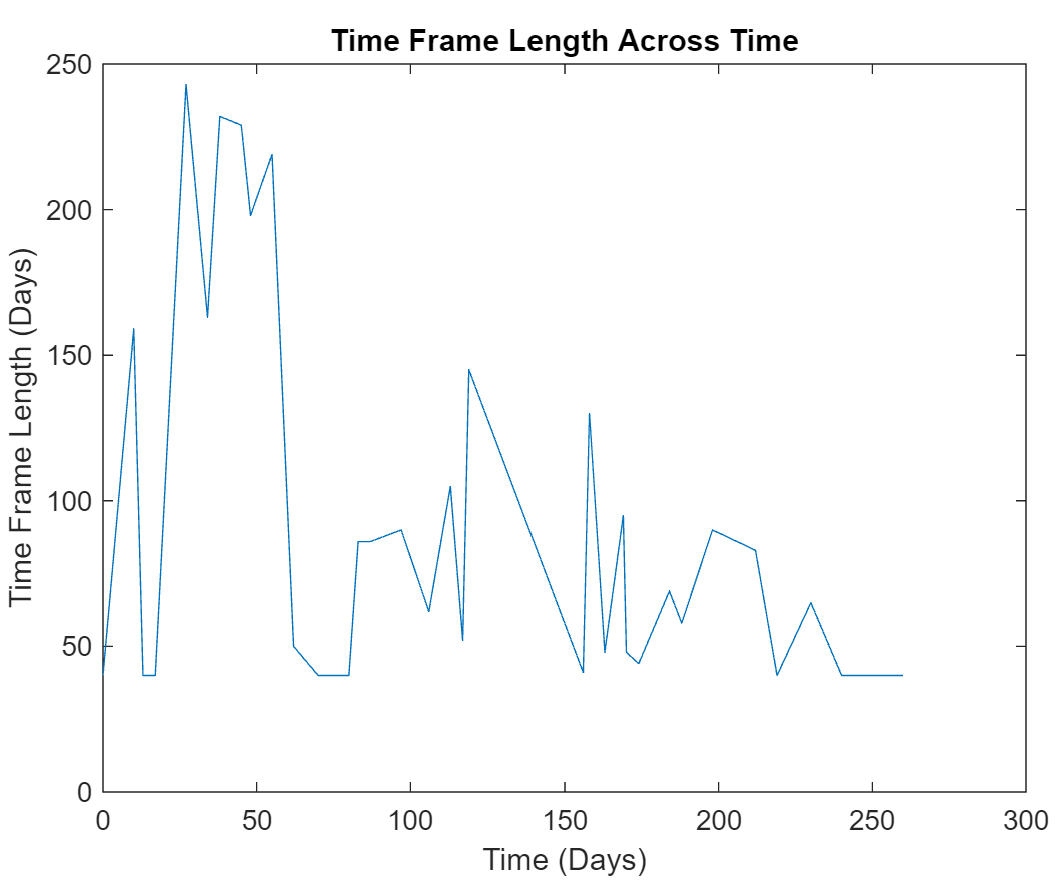
\includegraphics[width=120mm]{DeadliftConstants/TimeFrameLengthAcrossTime.png}
%    \caption{Time frame length over time. Note the general trend of increasing time frames, which is partly a function of the model having more data to work with as $t_t\to 0$.}
%    \label{fig:TimeFrameAcrossTime}
%\end{figure}

%TODO - add plot showing updated 1RM predictions

\section{Choosing A Time Frame: The General Case Through Sliding Window Analysis}
\label{sec:TimeFrameSlidingWindowAnalysis}

It turns out that the two 

\section{Analysis: Injuries, Setbacks, and Changes}
\label{sec:TimeFrameInjuriesAndChanges}

Section \ref{sec:TimeFrameDynamicTimeFrameAnalysis} was concerned with allowing the model to better adapt to a lifters current abilities. Using a 'local' measure of accuracy seemed to allow this, but proof that it does is needed.

An obvious place to check if the model is adapting to the lifters current abilities is the dates surrounding the lifters injury on $3/3/2022$. After an injury the model should respond by reducing the time frame so that only recent data is included, reflecting any drop in performance. A second place to check where the model adapts to a lifters current abilities is the dates surrounding any 1RM attempt. If the lifter peaked properly for the attempt then the models time frame should decrease leading up to the attempt and then re-increase again afterwards.

Looking at the time frame from $3/27/2022$-$5/30/2022$ the aforementioned patterns are present. The relevant data points and there respective time frames shown in table \ref{tab:TimeFrameNearCompetitionDeadlift}. From $3/27/2022$-$4/9/2022$ the time frame is trending downwards, indicating the model is adapting to the lifters post-injury capabilities. From $4/9/2022$-$4/28/2022$ the time frame re-increases, indicating the lifters abilities are returning. From $4/28/2022$-$5/5/2022$ the time frame decreases as the lifter approaches the competition on $5/5/2022$. Then, after the competition the time frame increases again. The behaviors of the time frame from table \ref{tab:TimeFrameNearCompetitionDeadlift} show the model is adapting to the lifters current abilities.

%An example of this is from the deadlift data between the dates of $4/2/2022$ and $5/30/2022$. The relevant data points and there respective time frames shown in table \ref{tab:TimeFrameNearCompetitionDeadlift}. Notice how as the competition approaches the models time frame begins to decrease, and afterwards the time frame re-increases. This is because the model was picking up on the lifters peak leading into the competition, where performance is temporarily boosted due to decreased fatigue levels.

\begin{table}[h]
    \centering
    \begin{tabular}{c|c}
        Date & $t_f$ \\
        \hline
        $3/27/2022$ & $145$ \\
        $3/29/2022$ & $52$ \\
        $4/2/2022$ & $105$ \\
        $4/9/2022$ & $62$ \\
        $4/18/2022$ & $90$ \\
        $4/28/2022$ & $86$ \\
        $5/2/2022$ & $86$ \\
        $5/5/2022$ & $40$ \\
        $5/15/2022$ & $40$ \\
        $5/23/2022$ & $50$ \\
        $5/30/2022$ & $219$
    \end{tabular}
    \caption{Time frame length over time when a lifter was peaking for a competition on $5/5/2022$. Notice how the time frame decreases as the competition approaches and then re-increases. This is proof the model can capture recent changes in training.}
    \label{tab:TimeFrameNearCompetitionDeadlift}
\end{table}

If an injury is severe enough, a lifter may loose all training progress and may never be capable of the same performance ever again. The data set (thankfully) does not have any data relating to a case like this, which makes it difficult to assess how quickly the model would respond to such a scenario. Even if the model does not respond quickly however, it does not make sense to include any data from the time before the injury occurred. To ensure this does not happen, the time frame can be limited to only include data from after the injury, creating a clean slate for the model to re-learn the lifters new abilities.

\section{Application: Predicting the Future?}
\label{sec:TimeFramePredictingTheFuture}

Up until now, the model was only making predictions about the current day. The next natural question is can the model make predictions further in the future? The answer is yes, but only based on the models current state. This is a pretty big 'but', as the models state will have changed by the time any future date is reached, thereby changing any predictions it would have made. To further complicate the issue, the more data is added to the data set between the current time and the predicted time the greater the potential is for the model state to vary drastically. This generally means the further out a prediction is in the future the less accurate it will be, and it is this reason that the predictions have been limited to only capture the next training session, and not reach beyond that. However, if changes to the models state can be predicted over time, then more valid predictions can be made about the future.

%TODO - make plot showing how this happens

%The next chapter will deal with finding patterns in the changing of state - a meta analysis
\section{
    Macrocycle
    \\
    \large{A Meta-Analysis}
}
\label{sec:Macrocycle}

%The previous section established what is possible for a lifter. This removed uncertainly about what could be done, however it must still be decided exactly what a lifter should do over the course of a training cycle to maximize results.

%TODO - introduce plots over time here
%\include{Mesocycle}

\appendix

\section{
    Appendix A
    \\
    \large{Data}
}
\label{sec:AppendixA}

TODO - figure out how to format data for paper/latex

\section{
    Appendix B
    \\
    \large{Potential Surface Graphs for Squat, Bench, and Deadlift}
}
\label{sec:AppendixB}

\begin{table}[h]
    \centering
    \begin{tabular}{c|c}
        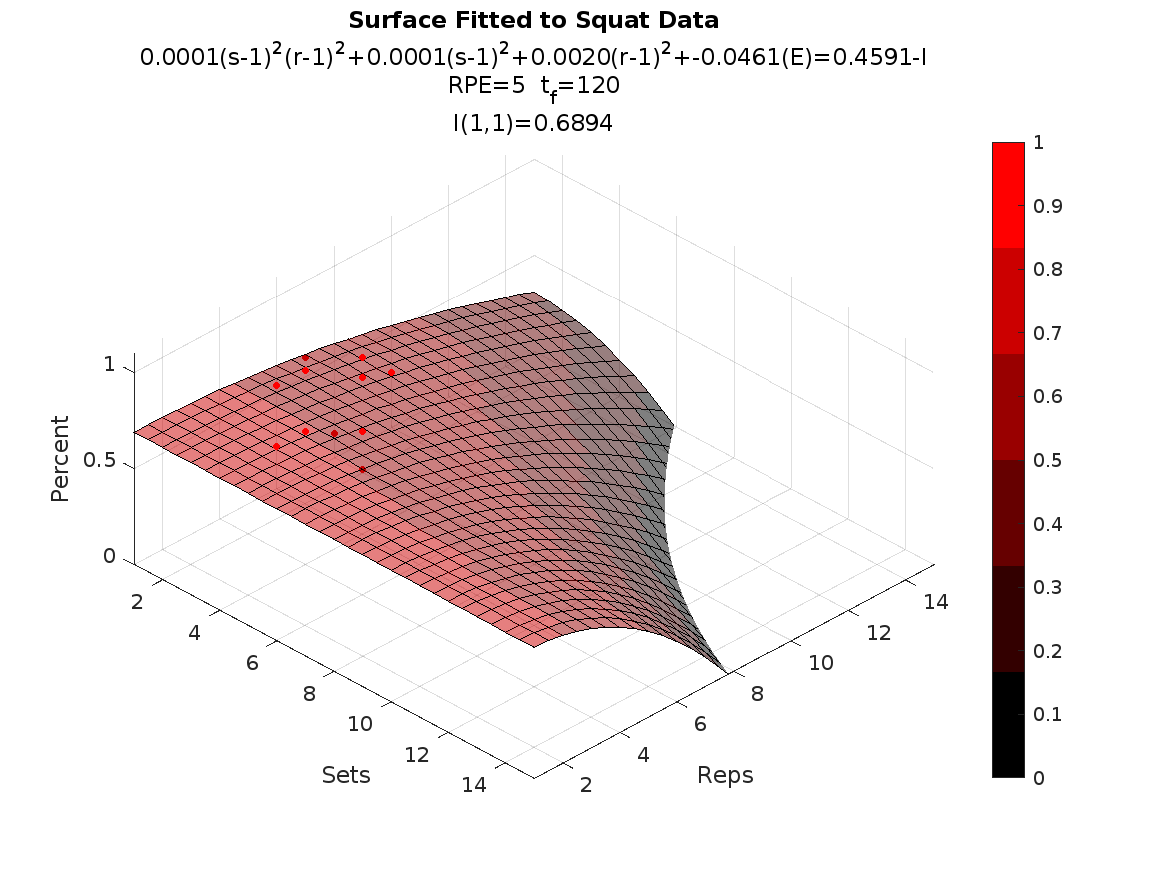
\includegraphics[width=78mm]{SquatSurface/5.png} &  
        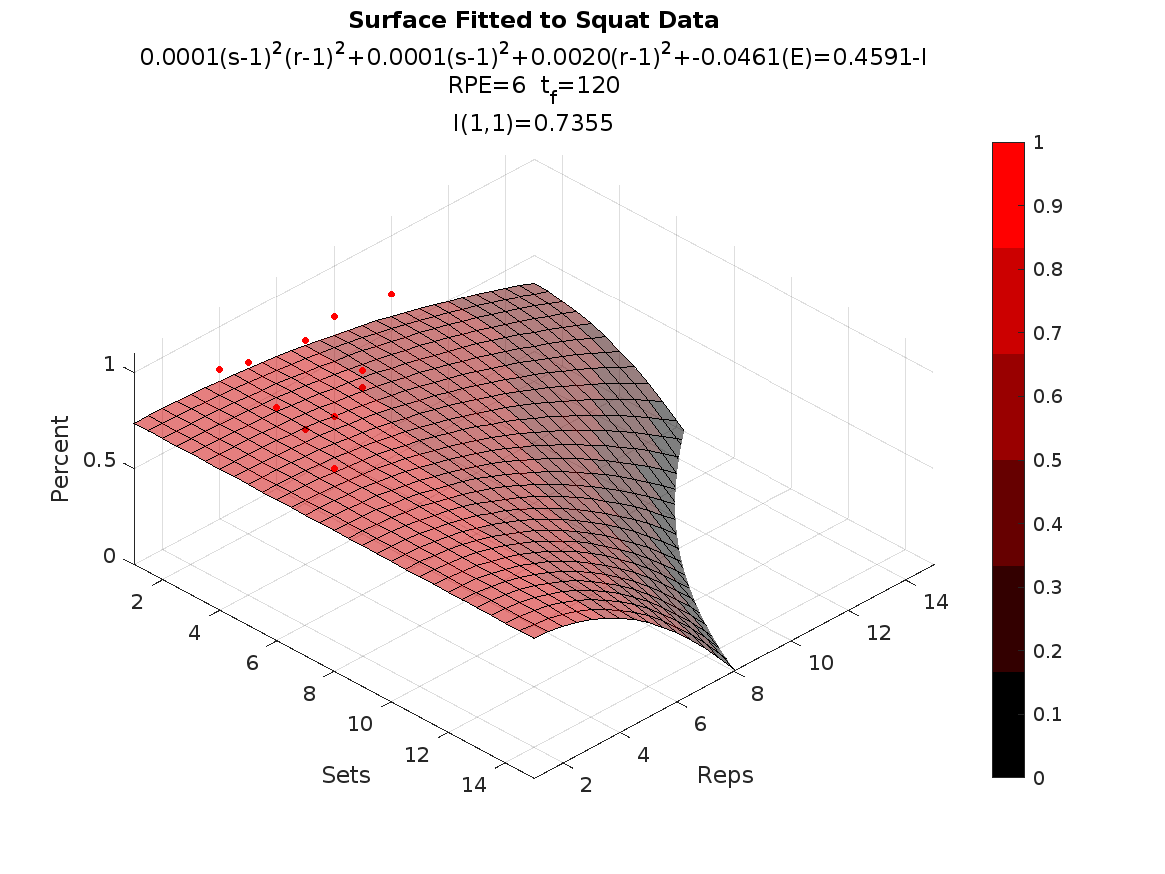
\includegraphics[width=78mm]{SquatSurface/6.png} \\
         
        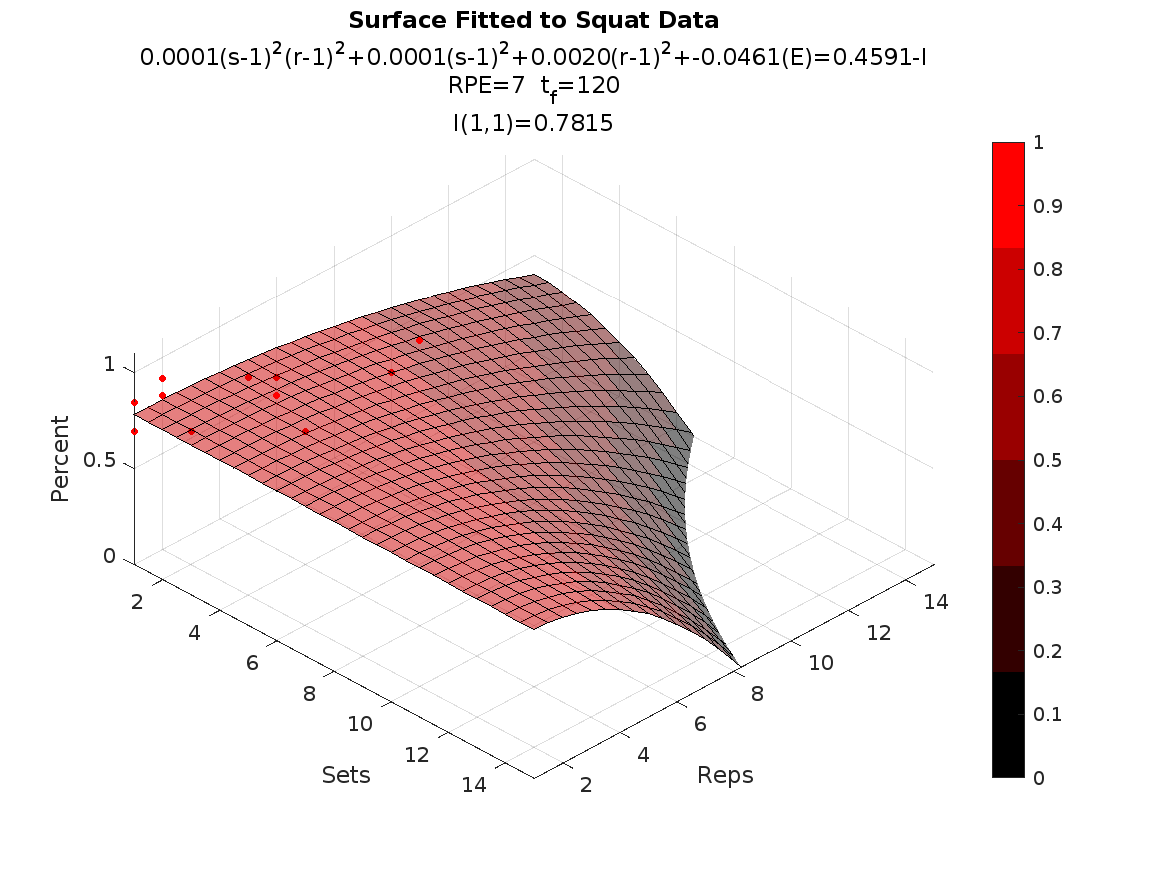
\includegraphics[width=78mm]{SquatSurface/7.png} &
        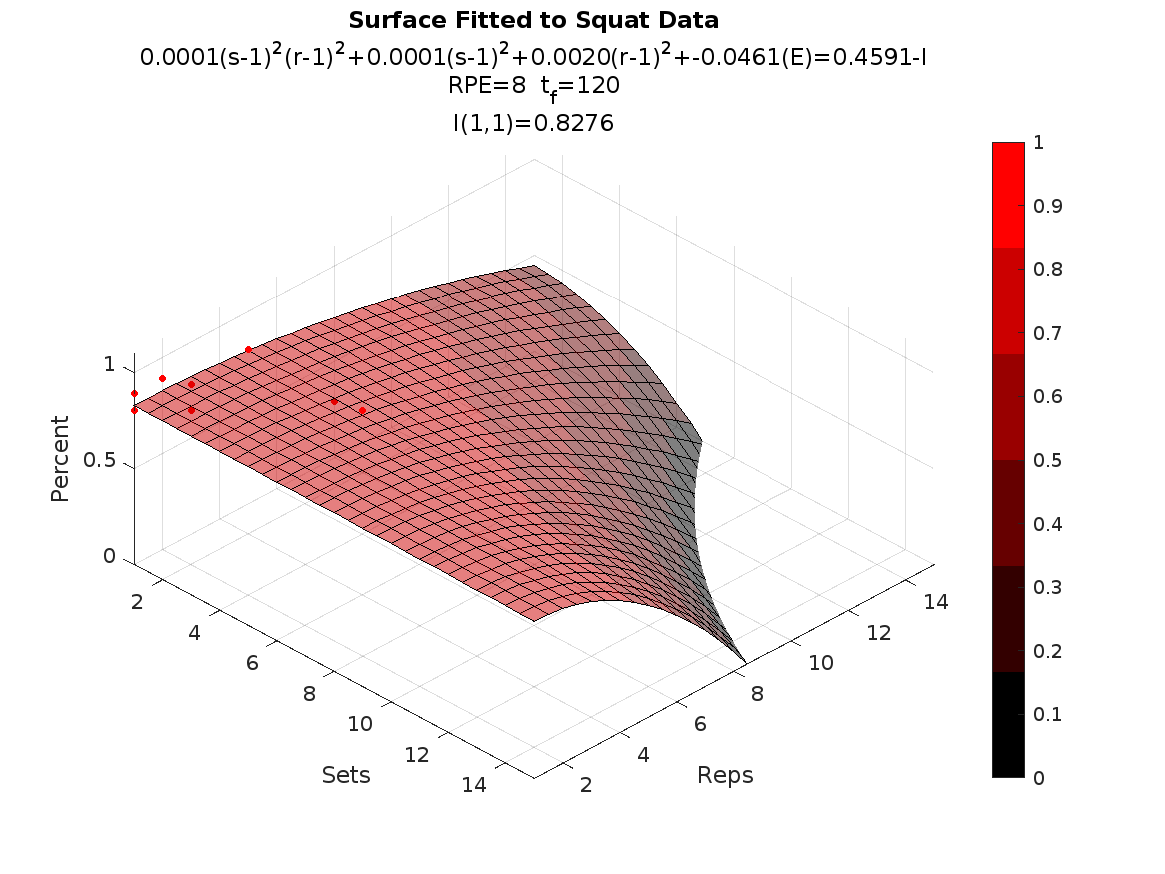
\includegraphics[width=78mm]{SquatSurface/8.png} \\
        
        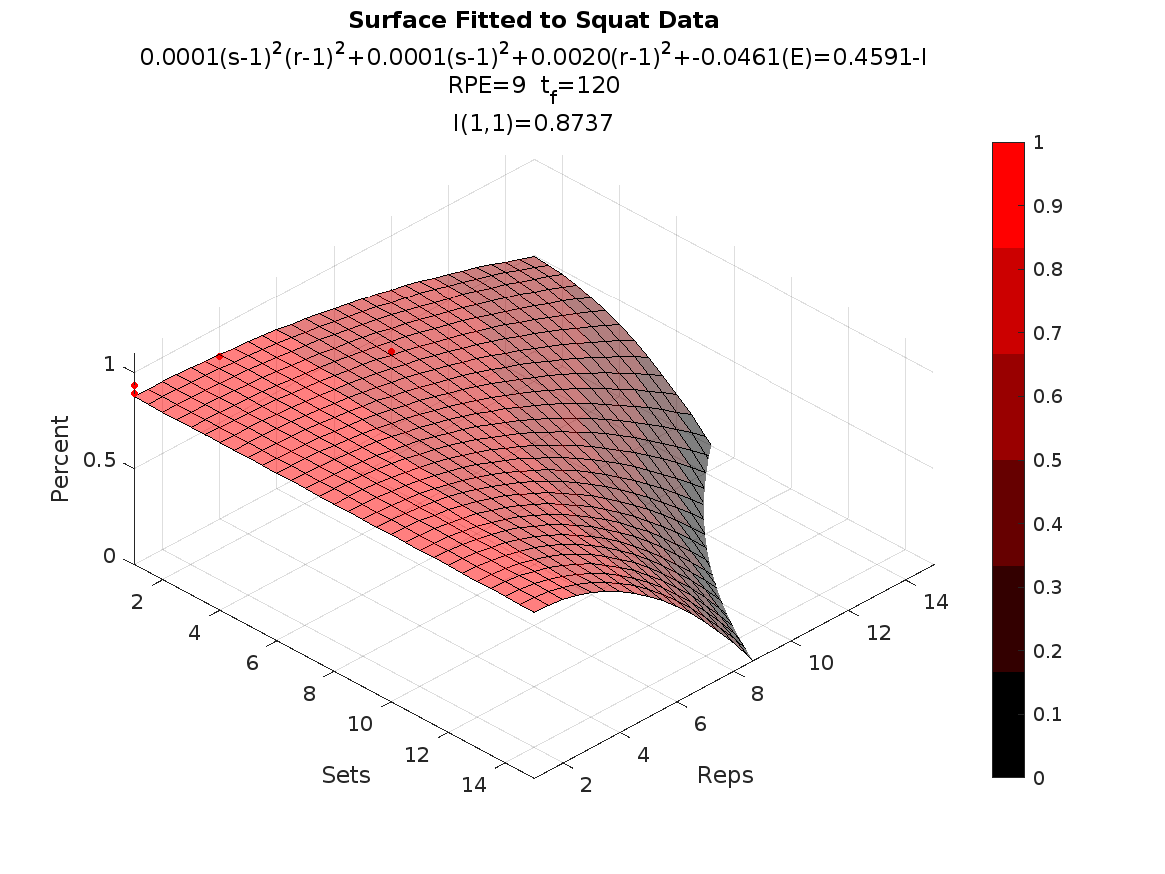
\includegraphics[width=78mm]{SquatSurface/9.png} &
        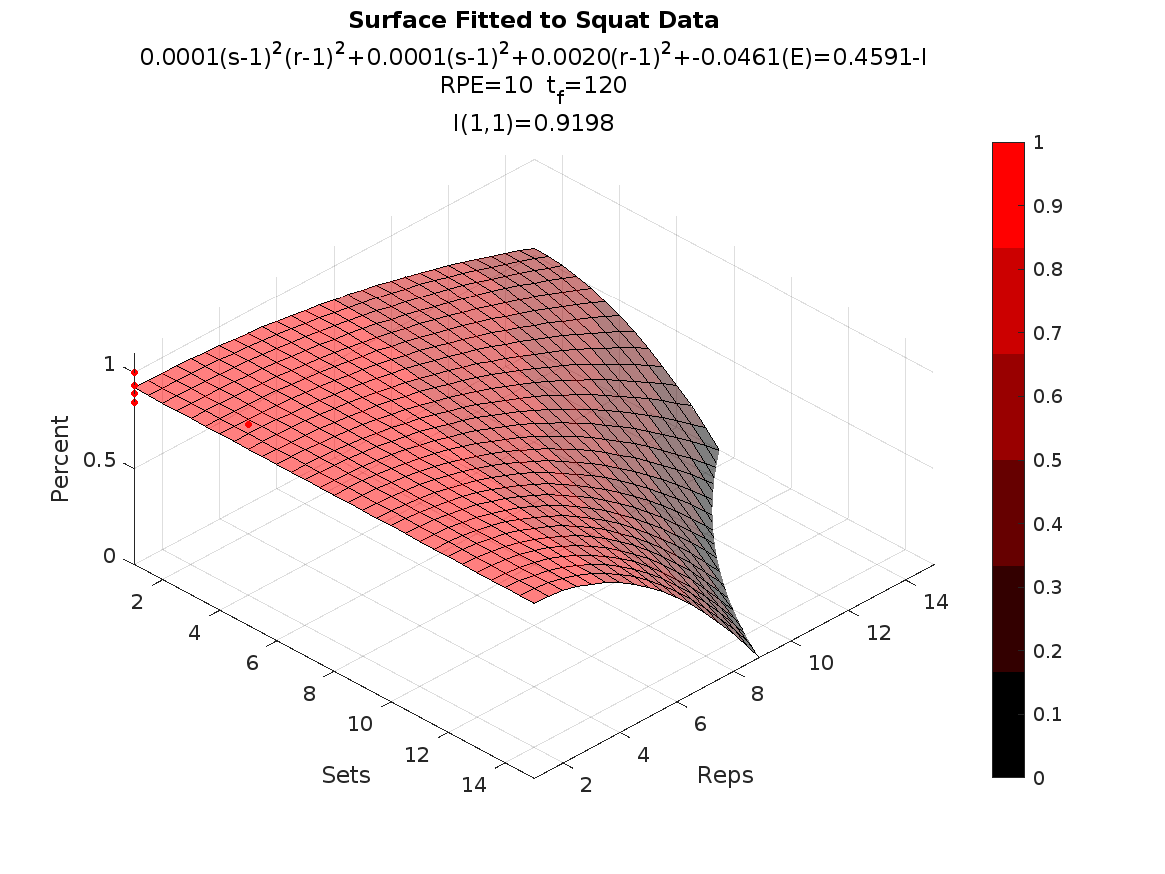
\includegraphics[width=78mm]{SquatSurface/10.png} \\
    \end{tabular}
    \caption{The potential surface fitted to squat data at various effort levels.}
    \label{tab:AppBSquatPotentialSurfaceAcrossEffort}
\end{table}

\begin{table}[h]
    \centering
    \begin{tabular}{c|c}
        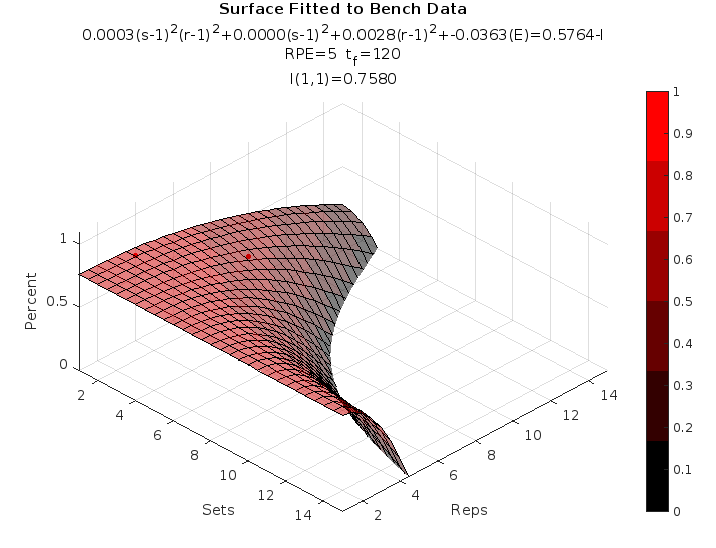
\includegraphics[width=80mm]{BenchSurface/5.png} &  
        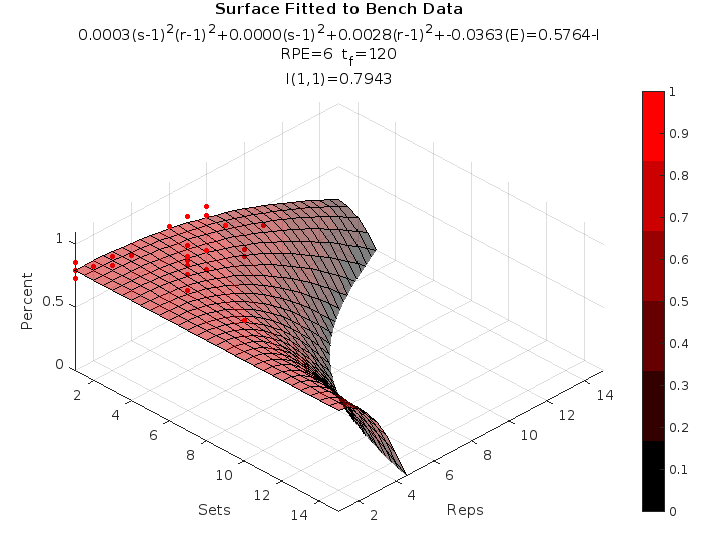
\includegraphics[width=80mm]{BenchSurface/6.png} \\
         
        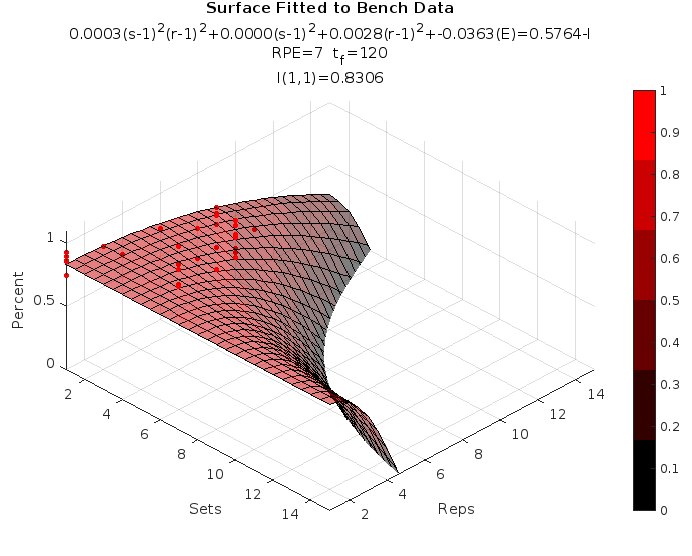
\includegraphics[width=80mm]{BenchSurface/7.png} &
        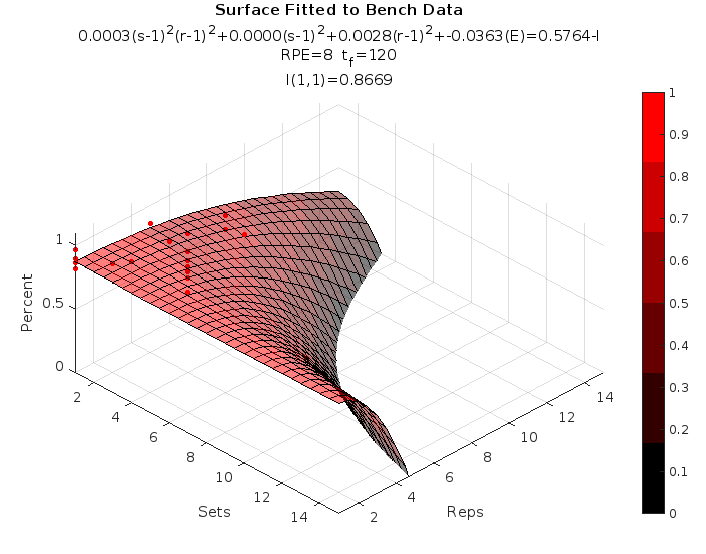
\includegraphics[width=80mm]{BenchSurface/8.png} \\
        
        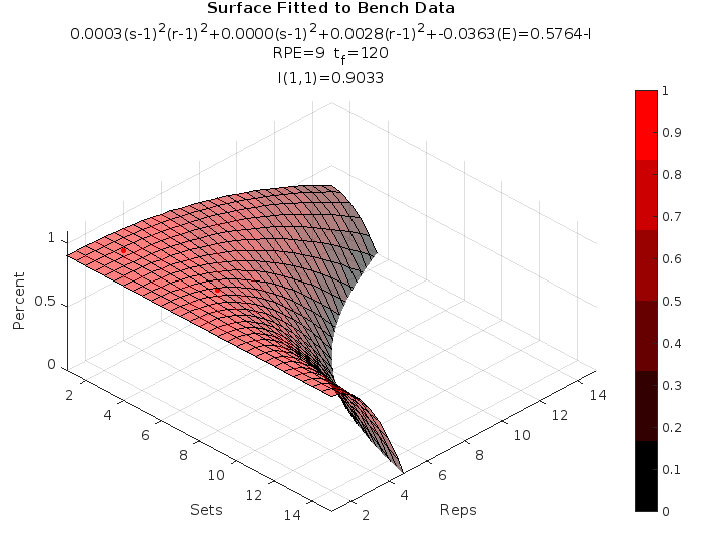
\includegraphics[width=80mm]{BenchSurface/9.png} &
        \includegraphics[width=80mm]{BenchSurface/10.png} \\
    \end{tabular}
    \caption{The potential surface fitted to bench data at various effort levels.}
    \label{tab:AppBBenchPotentialSurfaceAcrossEffort}
\end{table}

\begin{table}[h]
    \centering
    \begin{tabular}{c|c}
        \includegraphics[width=80mm]{DeadliftSurface/5.png} &  
        \includegraphics[width=80mm]{DeadliftSurface/6.png} \\
         
        \includegraphics[width=80mm]{DeadliftSurface/7.png} &
        \includegraphics[width=80mm]{DeadliftSurface/8.png} \\
        
        \includegraphics[width=80mm]{DeadliftSurface/9.png} &
        \includegraphics[width=80mm]{DeadliftSurface/10.png} \\
    \end{tabular}
    \caption{The potential surface fitted to deadlift data at various effort levels.}
    \label{tab:AppBDeadliftPotentialSurfaceAcrossEffort}
\end{table}

%\section{Weight Progression}

The weight progression model will define what weights a user will be attempting through the duration of the workout program, also known as a \textit{rotation}. What is needed is the weight progression for a \textit{single lift}. The model can then be generally applied to as many lifts as needed.

When thinking about weight progression, there are two time frames that need to be considered. The first is the length of the entire rotation, called the \textit{macro cycle}. The second time frame is each individual week, called the \textit{micro cycle}. Both of these time frames will be considered in the model.

The macro cycle is responsible for defining the weight progression over the entire rotation, without looking at day-to-day variations. The weight progression over the length of the rotation needs to be structured in a way to promote progress towards a new one rep max (1RM). In order to accomplish this, \textit{linear periodization} will be used. Linear periodization is a tried and true method for gaining strength. Weights will start off at a lower percentage of the users current one rep max and increase up to the users 1RM. This allows for a training stimulus to accumulate and result in an increased 1RM.
 
The micro cycle is concerned with the day-to-day variations from the macro cycle. For the micro cycle, the \textit{frequency} of a lift is very important. The frequency of a lift refers to how often a lifter will perform the same lift within a week. The percent of the 1RM being lifted throughout the week will need to decrease inversely with the frequency of a lift. This ensures that over training is avoided and reduces the chance of injury.

There are a few additional guiding principles that the model will need to support:
\begin{itemize}
    \item Deload: longer rotations will need a deload week to ensure the lifter is not overly fatigued by the end of the program. Shorter rotations will either not need a deload week or not need it to the same extent as longer rotations.
    \item Fatigue levels: Fatigue management is an important part of any good workout program. Without it progress can stall or even regress.
\end{itemize}

A relationship between the percentage of the users 1RM and time, $p(t)$, is needed. The models for the macro cycle, $p_{macro}(t)$, and micro cycle, $p_{micro}(t)$, will be considered individually and combined to create $p(t)$.

The model will be given:
\begin{itemize}
    \item The users max for a lift: $l_{1RM}$
    \item The users fatigue level: $f$ on a scale from $0-9$
    \item The frequency for a lift: $f_{req}$ on a scale from $1-7$
    \item The length of the rotation: $r_{ot}$
    \item A constant defining the maximum number of weeks a rotation can be: $r_{max}$
    \item A constant defining the minimum number of weeks a rotation can be: $r_{min}$
    \item Many users historical lifting data: $\{(r_{ot},b)_i\}_{i=0}^n$ where:
    \begin{itemize}
        \item $r_{ot} \equiv$ the length of the rotation
        \item $b \equiv$ the percentage back-off at the beginning of the rotation
    \end{itemize}
\end{itemize}


\subsection{Macro Curve}

The back-off, $b$, is related to the length of the rotation, $r_{ot}$. The argument that longer or shorter rotations need a greater backoff is one that can be side stepped by using the data supplied to the model. Knowing that $b$ and $r_{ot}$ are related is enough. A curve of best fit based on many users historical lifting data, $\{(r_{ot},b)_i\}_{i=0}^n$ will be used to define $b$.

\begin{equation}
    b(r)=Ar^2+Br+C
\end{equation}
\begin{equation*}
    E=\sum_{i=0}^n\left(b_i-Ar_i^2-Br_i-C\right)^2
\end{equation*}
\begin{equation*}
    \begin{split}
        \frac{\partial E}{\partial A}=&
        \frac{\partial}{\partial A}\sum_{i=0}^{n}\left(b_i-Ar_i^2-Br_i-C\right)^2
        =2\sum_{i=0}^{n}\left(-b_ir_i^2+Ar_i^4+Br_i^3+Cr_i^2\right)\\
        \frac{\partial E}{\partial B}=&
        \frac{\partial}{\partial B}\sum_{i=0}^{n}\left(b_i-Ar_i^2-Br_i-C\right)^2
        =2\sum_{i=0}^{n}\left(-b_ir_i+Ar_i^3+Br_i^2+Cr_i\right)\\
        \frac{\partial E}{\partial C}=&
        \frac{\partial}{\partial C}\sum_{i=0}^{n}\left(b_i-Ar_i^2-Br_i-C\right)^2
        =2\sum_{i=0}^{n}\left(-b_i+Ar_i^2+Br_i+C\right)\\
    \end{split}
\end{equation*}

\begin{equation*}
    \begin{bmatrix}
        \sum_{i=0}^{n}r_i^4 & \sum_{i=0}^{n}r_i^3 & \sum_{i=0}^{n}r_i^2\\
        \sum_{i=0}^{n}r_i^3 & \sum_{i=0}^{n}r_i^2 & \sum_{i=0}^{n}r_i\\
        \sum_{i=0}^{n}r_i^2 & \sum_{i=0}^{n}r_i & \sum_{i=0}^{n}1\\
    \end{bmatrix}
    \begin{bmatrix}
        A \\
        B \\
        C
    \end{bmatrix}
    =
    \begin{bmatrix}
        \sum_{i=0}^{n}b_ir_i^2 \\
        \sum_{i=0}^{n}b_ir_i \\
        \sum_{i=0}^{n}b_i \\
    \end{bmatrix}
\end{equation*}

\begin{equation}
    A=\frac{(B_3 A_2-A_3 B_2)(b_1 A_2-A_1 b_2)-(B_1 A_2-A_1 B_2)(b_3 A_2-A_3 b_2)}
           {(B_3 A_2-A_3 B_2)(C_1 A_2-A_1 C_2)-(B_1 A_2-A_1 B_2)(C_3 A_2-A_3 C_2)}
\end{equation}
\begin{equation}
    B=\frac{(B_1 A_3-A_1 B_3)(b_2 A_3-A_2 b_3)-(B_2 A_3-A_2 B_3)(b_1 A_3-A_1 b_3)}
           {(B_1 A_3-A_1 B_3)(C_2 A_3-A_2 C_3)-(B_2 A_3-A_2 B_3)(C_1 A_2-A_1 C_3)}
\end{equation}
\begin{equation}
    C=\frac{(B_2 A_1-A_2 B_1)(b_3 A_1-A_3 b_1)-(B_3 A_1- A_3 B_1)(b_2 A_1-A_2 b_1)}
           {(B_2 A_1-A_2 B_1)(C_3 A_1-A_3 C_1)-(B_3 A_1- A_3 B_1)(C_2 A_1-A_2 C_1)}
\end{equation}
\centerline{where}
\begin{equation*}
    \begin{bmatrix}
        \sum_{i=0}^{n}r_i^4 & \sum_{i=0}^{n}r_i^3 & \sum_{i=0}^{n}r_i^2\\
        \sum_{i=0}^{n}r_i^3 & \sum_{i=0}^{n}r_i^2 & \sum_{i=0}^{n}r_i\\
        \sum_{i=0}^{n}r_i^2 & \sum_{i=0}^{n}r_i & \sum_{i=0}^{n}1\\
    \end{bmatrix}
    \equiv
    \begin{bmatrix}
        A_1 & B_1 & C_1\\
        A_2 & B_2 & C_2\\
        A_3 & B_3 & C_3\\
    \end{bmatrix}
\end{equation*}
\begin{equation*}
    \begin{bmatrix}
        \sum_{i=0}^{n}b_ir_i^2 \\
        \sum_{i=0}^{n}b_ir_i \\
        \sum_{i=0}^{n}b_i \\
    \end{bmatrix}
    \equiv
    \begin{bmatrix}
        b_1 \\
        b_2 \\
        b_3 \\
    \end{bmatrix}
\end{equation*}

The deload week, $d$, needs to be placed such that there is sufficient time before and after it for linear periodization to occur. This naturally leads to placing the deload at the middle of the rotation.

\begin{equation}
    d=\left\lceil\frac{r_{ot}}{2}\right\rceil
\end{equation}

The deload halfway through the rotation necessitates a non-continuous solution for $p_{macro}(t)$. One way to create a  discontinuous function is by using a step function, which can be used to turn a series of other functions "on" and "off". \footnote{This step function is similar to the Dirac Delta function with the notable exception that the area underneath it is not guaranteed to be 1.}

\begin{equation}
    s_{tep}(t,s_{tart},e_{end})=
    \lim_{c \to +\infty} 
    \frac{1}{\left(\frac{2}{e_{end}-s_{tart}}\left(t-\frac{e_{end}+s_{tart}}{2}\right)\right)^c+1}
\end{equation}

The first function will need to be "on" over the domain $[0,d]$, and the second function will need to be "on" over the domain $(d,r_{ot}]$, creating the required discontinuity at $d$. A small constant will also be added to the start and end parameters to ensure that the step function has the correct values at each discontinuity. This is necessary because the value of the step function at each discontinuity is $\frac{1}{2}$ when it needs to be 1 for the model to work.

\begin{equation}
    p_{macro}(t)=f_1(t)s_{tep}(t,0-\epsilon,d+\epsilon)+
                 f_2(t)s_{tep}(t,d+\epsilon,r_{ot}+\epsilon)
\end{equation}
\centerline{where $\epsilon$ is a constant close to 0}

Two linear functions will be used to implement linear periodization. The first function will need to pass through the points $(0,b(r_{ot}))$ and $(d,p_1)$, where $p_1$is the highest percentage of the users 1RM that will be reached before the deload week occurs. The second function will need to pass through the points $(d,b(r_{ot}))$ and $(r_{ot},1)$.

\begin{equation*}
    f_1(t)=\frac{p_1-b(r_{ot})}{d}t+b(r_{ot})
\end{equation*}
\begin{equation}
    f_2(t)=\frac{1-b(r_{ot})}{r_{ot}-d}(t-d)+b(r_{ot})
\end{equation}

$p_1$ will be set to $95\%$ when $r_{ot}=r_{max}$ and will decrease in proportion to the length of the rotation until $p_1=b(r_{ot})$, removing the discontinuity at $d$. $p_1$ will need to decrease with the length of the rotation because the user will not have as long to prepare for a near maximal attempt at the halfway point of shorter rotations. $95\%$ was chosen because that is typically the closest lifters will get to setting a new 1RM without attempting a new 1RM.

In order to make $p_1$ approach $b(r_{ot})$ on shorter rotations as well as implement fatigue management, $f_1(t)$ will be changed to approach $f_2(t)$ as $r_{ot}\to r_{min}$ and as $f\to 9$. Fatigue management can be implemented here because $f_2(t)<f_1(t)$ when $t<d$. This means that if $f_1(t)$ approaches $f_2(t)$ then the user will be lifting a lower percentage of there 1RM, resulting in decreased stimulus and hence a way to manage fatigue. $f_1(t)$ will be redefined to support inverse percentage contributions from $f_2(t)$ and itself.

\begin{equation}
    f_1(t)=p_{contrib}\left (\frac{p_1-b(r_{ot})}{d}t+b(r_{ot}) \right)+
           (1-p_{contrib})f_2(t)
\end{equation}

Because $p_{contrib}$ depends on two variables, a geometric average is needed.

\begin{equation}
    p_{contrib}=\sqrt{\left( -\frac{f-9}{9} \right)
                      \left( \frac{r_{ot}-r_{min}}{r_{max}-r_{min}} \right)}
\end{equation}

With equations $1-10$ $p_{macro}$ is fully defined.

\subsection{Micro Curve}
The general idea for the micro curve is to define a function that can be multiplied by $p_{macro}$ to modify $p_{macro}$ so that it incorporates weekly lifting frequency. This can be done by defining $p_{micro}$ as percentages of $p_{macro}$.

Similar to $p_{macro}$, a step function is needed to turn a function "on" and "off". This step function will need to be cyclical to represent weekly changes in percentage. The period of the step function will need to equal one week in the weight progression model, forcing $l_{ength}=1$.

\begin{equation}
    s_{tepCyc}(t,l_{ength})=
        \lim_{c \to +\infty}
        \frac{1}{\left( \sin\left( \frac{2\pi}{l_{ength}}t-\frac{\pi}{2} \right) +1 \right)^c+1}
\end{equation}

Multiplying the cyclical step function by another function to define the decrease in percentage across a given week is necessary. It is also necessary to shift $p_{micro}$ by the same $\epsilon$ constant that $p_{macro}$ used so that the two equations coincide.

\begin{equation*}
    p_{micro}(t)=f_3(t)s_{tepCyc}\left( t-\frac{l_{ength}}{4}+\epsilon,1 \right)
\end{equation*}

Due to the cyclical nature of the step function, a trigonometric function is needed to define $f_3(t)$. Because $p_{micro}$ represents percentages of $p_{macro}$, $f_3(t)$ will be shifted so $f_3(t)\ge 0$. The period of $f_3(t)$ will need to match the period of $s_{tepCyc}$ so that the same series of percentages is repeated every week.

\begin{equation}
    f_3(t)=a_{mp}(f_{req})\sin\left( \frac{2\pi}{l_{ength}}\left( t-\frac{3l_{ength}}{4} \right) \right)+a_{mp}(f_{req})
\end{equation}

The amplitude of the trigonometric function will be used to define how large the backoff within the week will be. Due to the amplitude defining the backoff within the week, it will need to be inversely proportional with the weekly lifting frequency. This forces users with lower lifting frequencies to lift higher percentages of there 1RM and users with higher lifting frequencies to lift lower percentages of there 1RM. The amplitude will need to range from $0$ when $f_{req}=1$, representing no change from $p_{macro}$, to $0.25$ when $f_{req}=7$, representing $50\%$ of $p_{macro}$ after shifts are applied to $f_3(t)$. 

\begin{equation}
    a_{mp}(f_{req})=\frac{f_{req}-1}{24}
\end{equation}

The last consideration is to translate $p_{micro}$.

\begin{equation}
    p_{micro}(t)=f_3(t)s_{tepCyc}\left (t-\frac{l_{ength}}{4}+\epsilon,1\right)+(1-2a_{mp}(f_{req}))
\end{equation}

With equations $11-14$ $p_{micro}$ is fully defined.

\subsection{Combining the Curves and Interactive Graph}
The weight progression over the length of the rotation, $p(t)$, is then simply defined as follows.

\begin{equation}
    p(t)=p_{macro}(t)p_{micro}(t) \text{ for $0\le t \le r_{ot}$}
\end{equation}

An interactive graph of the weight progression model can be found \href{https://carmichaeljr.github.io/powerlifting-engine/}{here\footnote{https://carmichaeljr.github.io/powerlifting-engine/}}. Figure \ref{fig:Figure1.1} shows a screenshot of the interactive graph.

Figure \ref{fig:Figure1.2} demonstrates how the model responds to a decreased frequency. Note how the back-off on a per week level decreases with the lower frequency. On the extreme case when $f_{req}=1$ the model is simply reduced to $p_{macro}$. Figure \ref{fig:Figure1.3} showcases how the interactive model reacts to an increased fatigue level. Notice at $t=d$ how $p_1$ approaches $b(r_{ot})$. Figure \ref{fig:Figure1.4} showcases how the interactive model reacts to a shorter rotation length. Note how the emphasis on the deload week is less than in the longer rotation.

%---------------------------------------------------------------------------
\begin{figure}[h]
    \centering
    \includegraphics[scale=.23]{Figure1.1.png}
    \caption{A screenshot from the interactive graph demonstrating weight progression over time. The $t$ axis is scaled by $0.1$. $p_{macro}$ is shown in red and $p(t)$ is the black function. The deload week is highlighted in purple. The black dots are the values the user would follow assuming $f_{req}=7$.}
    \label{fig:Figure1.1}
\end{figure}
%---------------------------------------------------------------------------
\begin{figure}[h]
    \centering
    \includegraphics[scale=.14]{Figure1.2.png}
    \caption{A screenshot from the interactive graph demonstrating weight progression over time with decreased frequency. Note how the back-off on a per week level decreases with lower frequencies.}
    \label{fig:Figure1.2}
\end{figure}
%---------------------------------------------------------------------------
\begin{figure}[h]
    \centering
    \includegraphics[scale=.14]{Figure1.3.png}
    \caption{A screenshot from the interactive graph demonstrating the models adaptation to higher fatigue levels. Notice how $p_1$ approaches $b(r_{ot})$.}
    \label{fig:Figure1.3}
\end{figure}
%---------------------------------------------------------------------------
\begin{figure}[h]
    \centering
    \includegraphics[scale=.25]{Figure1.4.png}
    \caption{A screenshot from the interactive graph demonstrating the models adaptation to shorter rotations. Notice how $p_1$ approaches $b(r_{ot})$.}
    \label{fig:Figure1.4}
\end{figure}
%---------------------------------------------------------------------------
%\section{Set and Rep Scheme}

The set and rep scheme will define what sets and reps a user will be performing at a given percentage of the users 1RM. Again, what is needed is the sets and reps for a \textit{single lift}. The model can then be generally applied to as many lifts as needed.

When thinking about sets and reps, there are two steps to consider. The first is defining what combinations of sets, reps, and percentages are possible for the user to complete. Doing this will require defining a surface called the \textit{potential surface}. The second step to consider is selecting what combination of sets and reps the user will perform at each percentage. For a given surface there may be many set and rep options to choose from at a single percentage. This will require defining a line on the potential surface called the \textit{potential line} to select what combination to use for each percentage.

\textit{Volume}, the total amount of weight lifted by the user, needs to be considered when creating the potential surface. When the weight is low compared to the users current 1RM greater volume is required. Greater volume at lower percentages of the users 1RM aids in hypertrophy, skill acquisition, and motor skill refinement while setting the base for the heavier weights to come in the future. When the weight is approaching the users current 1RM, less volume is required. This is to avoid burnout and prevent injury when form breaks down at near maximal loads.

Volume is also an important factor for the potential line. It has been shown that the maximum volume needs to occur between $75\%$ and $85\%$ of the users current 1RM. Less than $75\%$ will not present a sufficient strength stimulus and greater than $85\%$ will be to taxing on the user and will cause burnout. The potential line will need to ensure that volume peaks within that range by selecting the appropriate path on the potential surface.

There are a few additional guiding principles that the model will need to support:
\begin{itemize}
    \item Volume tolerance: To much volume can lead to overuse injuries and not enough can stall progress. Some people respond well to high volume and other people respond well to low volume, requiring the model to adapt to the user.
    \item Fatigue levels: Fatigue management is an important part of any good workout program. Without it progress can stall or even regress.
\end{itemize}

A relationship between the percentage of the users 1RM and the combination of sets and reps is needed. The model will start by selecting the potential surface, $p(r,s)$, and then build the potential line, $l(p)$, off of that.

The model will be given:
\begin{itemize}
    \item The users max for a lift: $l_{1RM}$
    \item The users fatigue level: $f$ on a scale from $0-9$
    \item Historical lifting data: $\{(r,s,t,p)_i\}_{i=0}^{n}$ where:
    \begin{itemize}
        \item $r\equiv$ reps
        \item $s\equiv$ sets
        \item $p\equiv$ percentage of the appropriate 1RM that the sets and reps were performed at
        \item $t\equiv$ how long ago the lift was performed
    \end{itemize}
\end{itemize}


\subsection{Potential Surface}
The equation for the potential surface is shown below.
\begin{equation}
    p-1=-\frac{(r-1)^2}{a^2}-\frac{(s-1)^2}{b^2}
\end{equation}
The surface is reflected across the sr-plane and centered at $(1,1)$. By performing those two transformations, volume is high at low percentages and volume is low at high percentages. When $p=100\%$, there is only one option, $1$ set of $1$ rep, matching the users current abilities. The constants $a$ and $b$ need to be set so that the surface reflects plausible combinations of sets and reps for the user.

Solving for $p$ in the potential surface, setting $A=a^{-2}$ and $B=b^{-2}$, and adding a function to vary the weights of the bias with respect to time, $w(t)$, results in the following error equation, $E$.

\[ p=1-A(r-1)^2-B(s-1)^2 \]
\[ E=\sum_{i=0}^{n} w(t_i)\left(p_i-1+A(r_i-1)^2+B(s_i-1)^2 \right)^2 \]

The bias function $w(t)$ is needed because the potential surface needs to reflect the users current abilities. To make this happen, the bias function will place greater emphasis on lifts performed more recently and less emphasis on lifts performed in the past. The bias function will be explored in a separate section.

The error equation will need to be minimized to create the potential surface of best fit.

\begin{equation*}
    \begin{split}
        \frac{\partial E}{\partial A} & =
        \frac{\partial}{\partial A}
        \sum_{i=0}^{n} w(t_i)\left(p_i-1+A(r_i-1)^2+B(s_i-1)^2 \right)^2\\
        &=2\sum_{i=0}^{n} w(t_i)\left(p_i-1+A(r_i-1)^2+B(s_i-1)^2     \right)(r_i-1)^2\\
        &=2\sum_{i=0}^{n} w(t_i)\left(p_i(r_i-1)^2-(r_i-1)^2+A(r_i-1)^4+B(s_i-1)^2(r_i-1)^2\right)\\
        \frac{\partial E}{\partial B}
        &=2\sum_{i=0}^{n} w(t_i)\left(p_i(s_i-1)^2-(s_i-1)^2+A(r_i-1)^2(s_i-1)^2+B(s_i-1)^4\right)\\
    \end{split}
\end{equation*}

\begin{equation*}
    \begin{bmatrix}
        \sum_{i=0}^{n}w(t_i)(r_i-1)^4 & \sum_{i=0}^{n}w(t_i)(s_i-1)^2(r_i-1)^2\\
        \sum_{i=0}^{n}w(t_i)(r_i-1)^2(s_i-1)^2 & \sum_{i=0}^{n}w(t_i)(s_i-1)^4
    \end{bmatrix}
    \begin{bmatrix}
        A \\
        B
    \end{bmatrix}
    =
    \begin{bmatrix}
        \sum_{i=0}^{n}w(t_i)(r_i-1)^2(1-p_i) \\
        \sum_{i=0}^{n}w(t_i)(s_i-1)^2(1-p_i)
    \end{bmatrix}    
\end{equation*}

Solving the matrix results in the values for $a$ and $b$.

\begin{equation}
    a=A^{-\frac{1}{2}}
    =\left(
        \frac{p_1 B_2-B_1 p_2}{B_2 A_1-B_1^2}
    \right)^{-\frac{1}{2}}
\end{equation}
\begin{equation}
    b=B^{-\frac{1}{2}}
    =\left(
        \frac{A_1 p_2- p_1 A_2 }{B_2 A_1 -B_1^2}
    \right)^{-\frac{1}{2}}
\end{equation}
\centerline{where}
\begin{equation*}
    \begin{bmatrix}
        \sum_{i=0}^{n}w(t_i)(r_i-1)^4 & \sum_{i=0}^{n}w(t_i)(s_i-1)^2(r_i-1)^2\\
        \sum_{i=0}^{n}w(t_i)(r_i-1)^2(s_i-1)^2 & \sum_{i=0}^{n}w(t_i)(s_i-1)^4
    \end{bmatrix}
    \equiv
    \begin{bmatrix}
        A_1 & B_1\\
        A_2 & B_2
    \end{bmatrix}
\end{equation*}
\begin{equation*}
    \begin{bmatrix}
        \sum_{i=0}^{n}w(t_i)(r_i-1)^2(1-p_i) \\
        \sum_{i=0}^{n}w(t_i)(s_i-1)^2(1-p_i)
    \end{bmatrix}
    \equiv
    \begin{bmatrix}
        p_1 \\
        p_2
    \end{bmatrix}
\end{equation*}

With equations $16-19$, the potential surface is fully characterized. It is important to conceptualize that once this surface has been fitted to the users data, every point, every combination of sets, reps, and percentage, is in theory possible for the user to complete. This is the base that the following section will build off of.


\subsection{Potential Line}
A parametric equation relating $p$ to $s$ and $r$ following the potential surface is required, $l(p)=\left<s(r(p)),r(p),p\right>$.
In order to do this, the potential surface will conceptually be simplified to an infinite set of two-dimensional ellipses on the sr-plane. For each ellipse, $p$ is known. The equation for the ellipses is determined by solving the potential surface equation for $s$ in terms of $r$, treating $p$ as a constant.

\begin{equation}
    s(r)=1+b\sqrt{-\frac{(r-1)^2}{a^2}-p+1} \text{ where }r\ge1
\end{equation}

On each of these ellipses, a tangent line can be chosen in relation to $p$ so that when all the ellipses are combined and treated as a surface, the tangent line intersections with the surface create a continuous line up the side of the surface. This will require relating the tangent line slopes to $p$, $t_{slope}(p)$. The slope of the tangent line is calculated with a derivative.

\[ \frac{ds}{dr}=\frac{d}{dr}\left( 1+b\sqrt{-\frac{(r-1)^2}{a^2}-p+1}\right)=-\frac{b(r-1)}{a^2}\left( 1-\frac{(r-1)^2}{a^2}-p \right)^{-\frac{1}{2}} \]

Setting the slope equal to $t_{slope}(p)$ and solving for $r$ in terms of $t_{slope}(p)$ results in the equation $r(p)$.
\begin{equation}
    \begin{split}
        t_{slope}(p)&=-\frac{b(r-1)}{a^2}\left( 1-\frac{(r-1)^2}{a^2}-p\right)^{-\frac{1}{2}}\\
        t_{slope}(p)^2\left( 1-\frac{(r-1)^2}{a^2}-p \right)&=\frac{b^2}{a^4}(r-1)^2\\
        t_{slope}(p)^2(1-p)&=\frac{b^2}{a^4}(r-1)^2+\frac{t_{slope}(p)^2}{a^2}(r-1)^2\\
        r(p)&=\left(\frac{t_{slope}(p)^2(1-p)}{\frac{b^2}{a^4}+\frac{t_{slope}(p)^2}{a^2}}\right)^{\frac{1}{2}}+1
    \end{split}
\end{equation}

The equation for $t_{slope}(p)$ is shown below. This equation was chosen because it allows $t_{slope}$ to vary from large numbers at $p=0$ to $0$ at $p=1$, which is the range that the slope of the tangent line needs to be capable of covering. The constant $v_{peak}$ is left in the equation so that it can be set to ensure that volume peaks at $v_{max}$.
\begin{equation}
    t_{slope}(p)=e^{v_{peak}(1-p)}-p
\end{equation}

The equation to calculate volume is shown below.
\begin{equation}
    v(p)=r(p)s(r(p))
\end{equation}

The goal is to find $v_{peak}$ such that the maximum of $v(p)$ occurs at $v_{max}$. In order to do this, $v'(p)$ is needed. However, little is gained from substituting $r$ into $s$ besides a headache. The headache is even worse trying to take the derivative of $v(p)$ with respect to $p$, and worsens still when trying to solve that derivative for $v_{peak}$.\footnote{Try putting 
    "derivative of ((((e\char`^(c(1-x))-x)\char`^2*(1-x))/(b\char`^2/a\char`^4+(e\char`^(c*(1-x))-x)\char`^2/a\char`^2))\char`^(1/2)+1)*(1+b(-1/a\char`^2*(((((e\char`^(c*(1-x))-x)\char`^2*(1-x))/(b\char`^2/a\char`^4+((e\char`^(c*(1-x))-x)\char`^2)/a\char`^2))\char`^(1/2)+1)-1)\char`^2-x+1)\char`^(1/2))"
into Wolfram Alpha and you'll get an idea.} It is clear that numerical differentiation methods are needed. The five point formula for computing a first derivative is shown below.
\begin{equation}
    v'(p)\approx\frac{-v(p+2h_1)+8v(p+h_1)-8v(p-h_1)+v(p-2h_1)}{12h_1} \text{ where } h_1 \text{ is a number close to 0}
\end{equation}

Since numerical differentiation methods are in use, the way to solve for $v_{peak}$ changes. Instead of solving for $v_{peak}$ directly as with analog differentiation methods, a series of guesses will be made and then the best guess will be used as $v_{peak}$.

A set of guesses called $v_{potential}$ will take place of $v_{peak}$. This will redefine $t_{slope}(p)$ as a set of functions.
\begin{equation}
    v_{potential}=\{ 0,h_2,2h_2,3h_2,... \} \text{ where } h_2 \text{ is a number close to 0}
\end{equation}
\begin{equation}
    t_{slope}(p)=e^{v_{potential}(1-p)}-p
\end{equation}

Redefining $t_{slope}(p)$ as a set of functions also redefines $r(p)$, $s(p)$, $v(p)$, and $v'(p)$ as corresponding sets of functions. Plugging $v_{max}$ into $v'(p)$ results in a set of numbers that correspond to each functions value of $v'$ at $p=v_{max}$. From this set of numbers, the number closest to $0$ is found and the corresponding value of $v_{potential}$ is chosen to be $v_{peak}$. By doing this, the value in $v_{potential}$ that's closest to setting the maximum of $v(p)$ at $v_{max}$ is chosen.
\begin{equation}
        v_{peak}=\{ -\epsilon\le v'(v_{max})\le \epsilon: v_{potential}\}
\end{equation}
\begin{center}
    where $\epsilon$ is a number that guarantees $v'(v_{max})$ is sufficiently close to $0$ .
\end{center}

As stated before, volume needs to peak in the range of $75\%$-$85\%$ of the users 1RM. To determine the exact percentage where volume peaks within that range, fatigue needs to be taken into account. If the user is fatigued, volume will be peaked later in the program to increase recovery time. A simple linear equation relating $v_{max}$ and $f$, the users fatigue level from $0-9$, will suffice.
\begin{equation}
    v_{max}(f)=\frac{f}{90}+0.75 \text{ where }0\le f\le 9
\end{equation}

One final consideration has to be taken care of: sets and reps are whole numbers. The solution is to round up or down to the nearest integer. Again, a way to implement fatigue management has presented itself. If fatigue is below some threshold then round up, and if fatigue is at or above some threshold round down.
\begin{equation}
    l(p) =
    \begin{cases}
        \left<\lceil s(r(p))\rceil,\lceil r(p)\rceil,p\right> & \text{if $f<n$} \\
        \left<\lfloor s(r(p))\rfloor,\lfloor r(p)\rfloor,p\right> & \text{if $f\ge n$} \\
    \end{cases} 
\end{equation}


With equations $20$-$28$, the potential line is fully characterized, and the set and rep scheme is complete. 

\subsection{Interactive Graph}
An interactive graph of the sets and rep scheme can be found \href{https://carmichaeljr.github.io/powerlifting-engine/}{here\footnote{https://carmichaeljr.github.io/powerlifting-engine/}}. Figure \ref{fig:Figure2.1} shows a screenshot of the interactive graph. In the graph, squats are shown in blue, bench is shown in red, and deadlifts are shown in green.

Figure \ref{fig:Figure2.2} showcases how the interactive model reacts to an increased fatigue level. The overall volume is decreased, the peak in volume is pushed farther back in the program, and the potential line rounds down instead of up. All of these things combine together to create a strong fatigue management system that takes into account both volume and intensity.

%---------------------------------------------------------------------------
\begin{figure}[h]
    \centering
    \includegraphics[scale=.16]{Figure2.1.png}
    \caption{A screenshot from the interactive graph demonstrating the set and rep scheme. Squats are shown in blue, bench is shown in red, and deadlifts are shown in green. The large ovals represent the Potential Surface when $p=0$. The three curves near the origin are the potential lines. The darker lines near the potential lines are the potential lines but rounded up to the nearest integer.}
    \label{fig:Figure2.1}
\end{figure}
%---------------------------------------------------------------------------
\begin{figure}[h]
    \centering
    \includegraphics[scale=.25]{Figure2.2.png}
    \caption{A screenshot from the interactive graph demonstrating the models adaptation to higher fatigue levels. Notice the overall drop in volume and the delayed peak in volume.}
    \label{fig:Figure2.2}
\end{figure}
%---------------------------------------------------------------------------
%\section{Bias Function}
The bias function needs to capture the users current abilities from all the data given to the model. As with the previous two sections, a bias function is needed for a \textit{single lift}. The model can then be generally applied to as many lifts as needed.

When thinking about the bias function it has to be considered within the context of the error equation in the previous section. In order to capture the users current abilities the bias function will need to be $< 1$ for values that are considered current, reducing the errors from those data points. For values that are considered as not current the bias function will need to be $\ge 1$, increasing the errors from those data points. With this modification of errors the potential surface will be fit current data points better than non-current data points.

The phrase "current abilities" is rather ambiguous. Obviously, there is no one point that can define what is current and what is not for a user. The closest to discrete points in time being able to define what is current is the length of rotations. As such, current will be defined as $r_{ot}$, the length of the current rotation, weeks from the current date.

At the start of a new rotation data points from the users previous rotation will be used, assuming they are within $r_{ot}$ weeks of the current date. This makes sense because that data is the closest to representing the users current abilities. As the user continues their current rotation, data from the new rotation will supplant data from the old rotation, allowing for changes in the users current abilities to be reflected in the model. If, at the start of a rotation, the data from the user does not fall within $r_{ot}$ weeks from the current date then that data will be assigned a high error bias, which makes sense because abilities fade with time and a lack of practice.

A relationship between the time since a lift was performed and the bias of that lift is needed, $w(t)$.

The model will be given:
\begin{itemize}
    \item Historical lifting data: $\{(r,s,t,p)_i\}_{i=0}^{n}$ where:
    \begin{itemize}
        \item $r\equiv$ reps
        \item $s\equiv$ sets
        \item $p\equiv$ percentage of the appropriate 1RM that the sets and reps were performed at
        \item $t\equiv$ how long ago the lift was performed
    \end{itemize}
\end{itemize}

The bias function is shown below. An inverse cubic function is centered at $(r_{ot},1)$ and scaled appropriately to ensure that no biases are overly large or small.

\begin{equation}
    w\left(t\right)=r_{ot}^{-1}\left(t-r_{ot}\right)^{\frac{1}{3}}+1
\end{equation}

An inverse cubic function was chosen because is is not limited asymptotically, which means that the bias weights will not be limited to some constant as the data points get older. It was also chosen because the rate of increase is easily controlled to prevent biases that are overly large or small within any reasonable time frame.

\begin{equation*}
    \lim_{t \to +\infty}w(t)=
    \lim_{t \to +\infty}r_{ot}^{-1}\left(t-r_{ot}\right)^{\frac{1}{3}}+1=\infty
\end{equation*}
%\section{Volume}

As stated in the introduction, volume is already partially defined by the previous two sections. However, there are still a couple missing factors that need to be explored. The previous two sections outlined operations that need to occur for a single lift. This section is concerned with what needs to happen \textit{per workout program}, with many lifts being performed.

Volume will be split between four different categories. This is necessary because the reason for performing lifts in each category is different, necessitating a different approach to the volume.

\begin{enumerate}
    \item Main compound: Volume from squat, bench, and deadlift.
    \item Main compound accessory: Volume from variations of the squat, bench, and deadlift that do not significantly change the mechanics of the lift itself. These accessories can change variables such as the force curve or time under tension and are useful for breaking plateaus and forcing otherwise unattainable adaptations. Examples of these would be banded variations, paused variations, tempo variations, and variations with different bars.
    \item Compound accessory: Volume from multi-joint accessories that are not part of the main compound accessory group. These accessories are necessary to maintain symmetry and coordination as well as promote hypertrophy. Examples of these would be Bulgarian split squats, incline bench, and Romanian deadlifts.
    \item Accessory: Volume from single joint lifts. These accessories are necessary to focous on any specific weaknesses and promote active recovery. Examples of these would be machine work in general and some dumbbell exercises. Note that core work will be placed in this category due to it's relative ease of recovery.
\end{enumerate}


\subsection{Main Compound Volume}

Volume for this category is already full defined. The volume over time for a lift is shown below.

\begin{equation*}
    v_{mc}(t) = 
    \begin{cases}
        l_{1RM}p(t)\lceil s(r(p(t)))\rceil \lceil r(p(t))\rceil & \text{if $f<n$} \\
        l_{1RM}p(t)\lfloor s(r(p(t)))\rfloor \lfloor r(p(t))\rfloor & \text{if $f\ge n$} \\
    \end{cases} 
\end{equation*}

The set of 1RM's for all possible lifts in this category is defined as $MC$.
\begin{equation}
    MC=\{S_{1RM},B_{1RM},D_{1RM}\}
\end{equation}

The total volume would simply be the summation of volume across $MC$.

\begin{equation}
    v_{mc}(t) = 
    \sum_{l_{1RM}\in MC}
    \begin{cases}
        l_{1RM}p(t)\lceil s(r(p(t)))\rceil \lceil r(p(t))\rceil & \text{if $f<n$} \\
        l_{1RM}p(t)\lfloor s(r(p(t)))\rfloor \lfloor r(p(t))\rfloor & \text{if $f\ge n$} \\
    \end{cases} 
\end{equation}


\subsection{Main Compound Accessory Volume}

Volume for this category is similar to the previous category, but with more emphasis on rep work at lighter percentages. In order to enforce this, the percentage back-off at the start of the rotation will be greater for lifts in this category.

\begin{equation}
    b_2(r)=0.7b(r) \text{ where $b(r)$ is defined by equations $1-4$.}
\end{equation}

The set of 1RM's for all possible lifts in this category is defined as $MCA$. If the 1RM of a particular lift is not known a conservative estimate can be made by the user.

\begin{equation}
    MCA=\{\text{paused bench 1RM, paused squat 1RM, paused deadlift 1RM, etc}\dots\}
\end{equation}

The set of lifts that the user chooses to do, $l_{MCA}$, is subject to the constraints below. Typically, one exercise per main compound lift is chosen as an 'accessory' to work on a weak point of the main compound lift. This creates a size constraint on $l_{MCA}$.

\begin{equation}
    \begin{split}
        l_{MCA} & \subseteq MCA\\
        \left| l_{MCA} \right| & = \left| MC \right|
    \end{split}
\end{equation}

The total volume for this category is now fully defined.

\begin{equation}
    v_{mca}(t) = 
    \sum_{l_{1RM}\in l_{MCA}}
    \begin{cases}
        l_{1RM}p(t)\lceil s(r(p(t)))\rceil \lceil r(p(t))\rceil & \text{if $f<n$} \\
        l_{1RM}p(t)\lfloor s(r(p(t)))\rfloor \lfloor r(p(t))\rfloor & \text{if $f\ge n$} \\
    \end{cases} 
\end{equation}
\centerline{where $p(t)$ utilizes $b_2(r)$ in place of $b(r)$}

\subsection{Compound Accessory and Accessory Volume}
\label{sec:CompoundAccessoryVolume}
Volume for these two categories is not driven by 1RM attempts. Instead, it is used to form a basis of hypertrophy, which dictates high volume and lighter weights. Due to lifts in this category not being based on 1RM attempts, the model that has been outlined in the previous sections cannot be used.

Sets in these categories are typically in the range of $3-5$ and reps are typically in the range of $12-15$. The weight will need to be determined by the user due to the set and rep model relying on percentages of 1RM's. 1RM's are not known for lifts in these categories making the percentage of a 1RM also unknown. This will make fully defining volume for these categories impossible.

The set of lifts in each category is defined as follows.

\begin{equation}
    CA=\{\text{Bulgarian Split Squats, Incline Bench, Romanian Deadlifts, etc}\dots\}
\end{equation}
\begin{equation}
    ACC=\{\text{Core work, machine work, etc}\dots\}
\end{equation}

The set of lifts the user will choose to perform from each category, $l_{CA}$ and $l_{ACC}$, are subject to the constraints below.

\begin{equation}
    \begin{split}
            l_{CA} &\subseteq CA\\
            \left| l_{CA} \right| &= 3\left| MC \right|\\
            l_{ACC} &\subseteq ACC\\
            \left| l_{ACC} \right| &= 2\left| MC \right|
    \end{split}
\end{equation}


\subsection{Interactive Graph}

Figure \ref{fig:Figure3.1} shows the total volume over different rotation lengths for one exercise. The purple lines represent main compound volume and main compound accessory volume. The green line is the summation of the two purple lines, representing volume across a rotation. Note how, in general, volume peaks early and quickly regains after the deload week so that it can taper off again as the user approaches a 1RM attempt. Note how for the shorter rotation the volume curve approaches having a single peak. This is due to shorter rotations not having as significant of a deload week.

Figure \ref{fig:Figure3.2} shows how volume reacts to increased fatigue levels. The total amount of volume decreases across the length of the rotation. Note how the peak in volume is pushed closer to the end of the program to aid in recovery now.

The properties just pointed out are not a direct result from any one equation forcing the behaviors to exist. They are a result of the considerations taken into account when making the weight progression and set and rep scheme. This is important because the volume graphs are showing that the actions taken to manage volume previously are working as intended.

%---------------------------------------------------------------------------
\begin{figure}[h]
    \centering
    \includegraphics[scale=.5]{Figure3.1.png}
    \caption{A screenshot from the interactive graph showing volume over different rotation lengths for one exercise. The solid lines are the fractional set and rep values produced from the model and the lighter lines are rounded set and rep values also produced according to the model.}
    \label{fig:Figure3.1}
\end{figure}
%---------------------------------------------------------------------------
\begin{figure}[h]
    \centering
    \includegraphics[scale=.2]{Figure3.2.png}
    \caption{A screenshot from the interactive graph demonstrating how the volume drops with higher fatigue levels. Note how the peak in volume is pushed closer to the end of the rotation to aid in recovery now.}
    \label{fig:Figure3.2}
\end{figure}
%---------------------------------------------------------------------------
%\section{Max Prediction}

A model is no use if it cannot be used to make predictions. One common prediction lifters make is there current 1RM for a lift. Going back to the sets and reps scheme, slight modifications can be made to create an estimation of the users 1RM.

As data is collected on the users current rotation, the potential surface will diverge from what it originally was, representing a change in the users abilities. If this new potential surface is not constrained to peak at $p=1$, the users estimated new 1RM can be represented as a percentage of the users current 1RM. To allow for this a new constant, $n_{max}$, is added and solved for.

\begin{equation*}
    p-n_{max}=-\frac{(r-1)^2}{a^2}-\frac{(s-1)^2}{b^2}
\end{equation*}

Solving for $p$ in the potential surface, setting $A=a^{-2}$ and $B=b^{-2}$, and adding a function to vary the weights of the biases with respect to time, $w(t)$, results in the following error equation, $E$. Recall that $A$ and $B$ are known.

\[ p=n_{max}-A(r-1)^2-B(s-1)^2 \]
\[ E=\sum_{i=0}^{n} w(t_i)\left(p_i-n_{max}+A(r_i-1)^2+B(s_i-1)^2 \right)^2 \]

The error equation will need to be minimized to create the surface of best fit.

\begin{equation*}
    \begin{split}
        \frac{d E}{d n_{max}}
        &=2\sum_{i=0}^{n}w(t_i)\left( -p_i+n_{max}-A(r_i-1)^2-B(s_i-1)^2 \right)
    \end{split}
\end{equation*}

Solving for $n_{max}$ results in the following equation.

\begin{equation}
    n_{max}=\frac{\sum_{i=0}^{n}w(t_i)p_i+
                  A\sum_{i=0}^{n}w(t_i)(r_i-1)^2+
                  B\sum_{i=0}^{n}w(t_i)(s_i-1)^2}{\sum_{i=0}^{n}w(t_i)}
\end{equation}

The predicted new 1RM is then simply the product of the users current 1RM and $n_{max}$.

\begin{equation}
    n_{1RM}=n_{max}l_{1RM}
\end{equation}

An interactive graph of the max prediction can be found \href{https://carmichaeljr.github.io/powerlifting-engine/}{here\footnote{https://carmichaeljr.github.io/powerlifting-engine/}}. Figure \ref{fig:Figure4.1} shows how the potential surface diverges with the addition of new data. The first set of data creates the potential surface shown in red. The second set of data is the first set of data with more recent training data added to it and is shown in green. For the first set of data the estimated 1RM is 444 lbs. For the second set of data the estimated 1RM is 475 lbs.\footnote{The exact data used is available in the interactive graph under the data folder.}

%---------------------------------------------------------------------------
\begin{figure}[h]
    \centering
    \includegraphics[scale=.25]{Figure4.1.png}
    \caption{A screenshot from the interactive graph demonstrating the change in the potential surface. The first set of data creates the potential surface shown in red. The second set of data is the first set of data with more recent training data added to it and is shown in green. The original max prediction is 444 lbs, and the new one is 475 lbs.}
    \label{fig:Figure4.1}
\end{figure}
%---------------------------------------------------------------------------
%\section{Identifying Training Patterns}

Another common thing that lifters will do is attempt to find patterns within there training, both across time and per lift. A model can be used to help the user identify trends in there training. Note that the model outlined in this section is untested because the large amount of data that it would require to implement was not available during the writing of this paper.

A lifter usually will break up their training history into two distinct categories and then look for patterns on a per lift basis. The first category is "good" training periods when progress was made, called a \textit{progression state}. The second is "bad" training periods when progress was either not made or lost, called a \textit{regression state}. The model must make this distinction so that progress states and regression states can be analyzed separately. 

The model will also need to identify patterns based on data from a single lift. That is to say, when a user makes progress on there squat the model should identify patterns that are different from when progress is made on deadlifts.

A relationship between a chosen lift, $l_{chosen}$, and the other lifts is needed. The model will start by defining a function relating 1RM's from $l_{chosen}$ and time, $S(t,l_{chosen})$, to identify progression and regression states. From there, the model will seek to find patterns in lifts other than $l_{chosen}$ related to progress in $l_{chosen}$.

The model will be given:
\begin{itemize}
    \item A users historical lifting data: $\{(l,t)_i\}_{i=0}^n$ where:
    \begin{itemize}
        \item $l \equiv$ the exercise that was performed
        \item $t \equiv$ how long ago the lift was performed
    \end{itemize}
    \item A users historical lifting data: $\{(l_{Rot1RM},t)_i\}_{i=0}^n$ where:
    \begin{itemize}
        \item $l_{Rot1RM} \equiv$ a users maximum for a particular lift per rotation
        \item $t \equiv$ how long ago the lift was performed
    \end{itemize}
\end{itemize}

\subsection{Progression and Regression States}
Progress, as defined on a per lift basis, is when the 1RM for that lift increases. In order to capture this, a cubic spline can be fit to the users historical lifting data relating 1RM's of $l_{chosen}$ per rotation and time, $\{(l_{Rot1RM},t)_i\}_{i=0}^n$, creating $S(t,l_{chosen})$. Whenever $S'(t,l_{chosen})>0$ it will mean progress is being made.\footnote{The process of defining a cubic spline is long and also widely available. The derivation is skipped here for brevity.}

\subsection{Identifying Patterns}
With progress defined in relation to $l_{chosen}$, patterns can now be found in the data. Throughout the rest of this section, $P$ is the set of data points from the users historical lifting data, $P=\{(l,t)_i\}_{i=0}^n$. $P_t$ refers to the time component of a data point from the users historical lifting data, and $P_l$ corresponds to the lift component from the users historical lifting data.

The first pattern to find is lifts that have a positive correlation with progress for $l_{chosen}$. In order for a lift to have a positive correlation with progress for $l_{chosen}$ it will need to be performed often when progress is being made. This can be found through a simple ratio between the number of times the lift was performed during a progression state and the total time spent in a progression state across the users lifting career, creating a rating from $0-1$ on how well a lift correlates with progress.

\begin{equation}
    l_{ProgCoor}(l)=\frac{\left| \{ P | P_l=l \land S'(P_t,l_{chosen})>0 \} \right|}
                         {\left| \{ P | S'(P_t,l_{chosen})>0 \} \right|}
\end{equation}

In order to find similar patterns in a regression state for $l_{chosen}$ all that's needed is to change is the conditional.

\begin{equation}
    l_{RegCoor}(l)=\frac{\left| \{ P | P_l=l \land S'(P_t,l_{chosen})\le0 \} \right|}
                        {\left| \{ P | S'(P_t,l_{chosen})\le0 \} \right|}
\end{equation}

The second pattern to find is how a lifts frequency corresponds with progress for $l_{chosen}$. The average frequency of a lift when a user is in a progress state is needed. To start with, the frequency of a lift is needed for a given week.

\begin{equation}
    l_{freq}(l,w_{eek})=\frac{
                    \left| \left\{ P | \left\lfloor \frac{P_t}{7} \right\rfloor=w_{eek} \land 
                    P_l=l \land
                    S'(P_t,l_{chosen})>0 \right\} \right|
                }{
                    7
                }
\end{equation}

With the frequency of a lift for a given week, the average frequency can then be calculated. Finding the average lifting frequency while a user is in a regression state does not make sense because a user will have one optimal lifting frequency and many sub-optimal lifting frequencies, making an average meaningless.

\begin{equation}
    l_{ProgFreqCoor}(l)=\frac{
                            \sum_{
                            \substack{
                                    w_{eek}\in \left\{ \left\lfloor \frac{P_t}{7} \right\rfloor \right\}\\
                                    S'(7w_{eek},l_{chosen})>0
                                }
                            }
                        l_{freq}(l,w_{eek})
                        }{
                            \left|\left\{ \left\lfloor \frac{P_t}{7} \right\rfloor | S'(P_t,l_{chosen})>0 \right\}\right|
                        }
\end{equation}

Frequency was left as a input to the weight progression model because the above prediction relies on large amounts of data which is not available from a new user. Initially, a user will select a frequency that they find appropriate, then, as the model collects more data, it will be able to recommend an optimal frequency to the user.
%\section{Adaptation to the User}

The goal of this paper is to define a workout program that adapts to help a user lift within their optimal constraints. The model outlined does this in several ways.

\subsection{Volume Tolerance}
Volume forms the base for heavy 1RM attempts. If volume increases, forming a larger base, then chances are a new 1RM is in the users future. \footnote{This is not always true for advanced lifters. For beginners this is almost always the case however.} As such, volume should be increased within the users abilities to promote progress. The model does this in two ways.

The first way volume is increased simply by increasing the weights lifted. When a user sets a new 1RM the percentages from the weight progression model remain constant, but the value those percentages are in relation to increases. This will result in heavier sets across the board, thereby increasing volume. This is a very typical way to increase volume in other powerlifting programs, making it important that it is implicit in the weight progression model.

The second way volume is increased is through higher numbers of sets and reps. The set and rep scheme rounds sets and reps up to the nearest integer, given that fatigue is below a certain threshold. This may seem like a trivial fact but it has a very important implication: it promotes an increase in volume over time. If a user completes the rounded up sets and reps then a new data point will be generated that the potential surface will fit to. If this is performed across an entire rotation then the potential surface will be pushed out to match the users increased tolerance to volume. If this is repeated across several rotations the sets and reps will continually be rounded up and the end result will be a significant increase in volume.

Volume is important, but it is not the only training factor and there will reach a point where more volume will do more harm than good. As such, a way to decrease the volume needs to be present in the model. 

One way this is done is through fatigue management. If a user is feeling fatigued then the prescribed number of sets and reps will decrease, and if a very high fatigue state is reached the model will start to round sets and reps down instead of up. If a user maintains the same fatigue state throughout the length of the rotation then sets and reps will be decreased across the board, decreasing volume for the entire rotation. The decrease in volume will push the potential surface in reflecting the users decrease in tolerance to volume. This will then result in less volume for the next rotation, which is likely a good thing if the user had a high level of fatigue throughout the entire length of the previous rotation.

The second way volume can decrease is if a user starts to fail lifts. This obviously represents a sub-optimal lifting state for the user so it is important that the model reacts to it. Again, the same concept applies where the potential surface will be pushed in from new data points where the user failed a set, resulting in decreased volume. If a user starts failing lifts it is a clear sign they are fatigued, and they should increase their fatigue level in the model so it can appropriately adjust and decrease volume. If this is done the user can avoid failing lifts all together.

It should be clear that there is a tug of war between the model pushing the user to do more and the user telling the model that they cannot, keeping the user lifting withing their optimal constraints.


\subsection{General Flexibility}
There are some training parameters that the model outlined in this paper cannot account for such as stresses levels outside of the gym, time management, and injuries. Because the model cannot directly adapt to these parameters room was left in the model for the users input.

The model outlined in this paper allows the user to change several parameters:
\begin{enumerate}
    \item The length of the rotation
    \item There fatigue level
    \item The frequency of a particular lift
\end{enumerate}

These parameters allow the user to dynamically change there training, even in the middle of a rotation. The model can supply recommended values for some of these parameters, but those recommendations do not account for the factors discussed earlier. The user can choose to accept the recommendation or modify it based on the outside knowledge they have.
%

\printbibliography[heading=bibintoc,title={References}]

\end{document}